\documentclass[10pt,a4paper,twocolumn]{article}

\usepackage[margin=1.8cm]{geometry}
\usepackage[cmex10]{amsmath}
\usepackage{amssymb,bm}
\usepackage{array}
\usepackage{booktabs}
\usepackage{graphicx}
\usepackage{hyperref}
\usepackage{microtype}
\usepackage{siunitx}

\hypersetup{colorlinks=true, linkcolor=blue, citecolor=blue, urlcolor=blue}
\sisetup{per-mode=symbol}
\setlength{\columnsep}{0.7cm}
\newcommand{\chfour}{\ensuremath{\mathrm{CH_4}}}
\newcommand{\cv}{\ensuremath{C_V}}
\newcommand{\cpheat}{\ensuremath{C_P}}

\title{Efficient Heat Capacity of Methane-Loaded MOF-5 with Classical Molecular Dynamics and Machine-Learned Hessians}
\author{\textit{Author name}}
\date{\today}

\begin{document}

\begin{titlepage}
	\centering
    
\includegraphics[width=0.5\linewidth]{figures/epfl.png}\\[0.25cm] 	% University Logo
    \textsc{\LARGE École Polytechnique Fédérale de Lausanne}\\ \vspace{\fill}
    \textbf{\textsc{\fontsize{50}{50}\selectfont Advanced electronic structure calculation of semiconductors}}\\ \vspace{\fill}		
	\textsc{\LARGE Physics project II}\\[0.4cm]
	\rule{\linewidth}{0.2 mm} \\[0.5 cm]
	Lucas De Almeida Kloss \\[2cm] \today
\end{titlepage}

\tableofcontents

\pagebreak

\begin{abstract}
This report develops an efficient heat-capacity workflow for methane-loaded
MOF-5 using a machine-learned interatomic potential (MLIP). Classical
flexible-cell NPT molecular dynamics (MD) samples the loaded system and retains
anharmonic methane and host--guest motion. Automatic differentiation (AD)
through the matching PET-JAX model provides sparse Cartesian Hessians and
normal-mode frequencies at quenched reference structures, which must be
validated as local minima. Rather than reproduce the
reference simulations with an MLIP, the workflow applies the hybrid
approximation proposed by Kapil \emph{et al.}: the loaded-system classical
anharmonic heat capacity is corrected by the difference between quantum and
classical harmonic heat capacities evaluated for the same loaded composition
and PET potential. The already-equilibrated empty MOF-5 structure is relaxed
directly and evaluated with one reference Hessian; no empty-framework MD
campaign is required. The resulting low-temperature and model-dependent
accuracy must be validated for the selected MLIP. Finite-trajectory sampling
error and correlated classical--harmonic model spread are evaluated with a
last-layer prediction-rigidity (LLPR) ensemble. The available PET-MAD and
PET-SOL calculations cover 50, 100, and 150 methane molecules and give
exploratory room-temperature hybrid values near 0.93, 1.07--1.08, and
\SI{1.16}{J\per g\per K}, respectively. Imaginary Hessian modes, incomplete
relaxation, production drift, and strong sensitivity to uncertainty
propagation prevent interpreting these values as converged predictions.
Variation across independently quenched minima remains unestimated.
\end{abstract}

\section{Scientific motivation and scope}

Metal--organic frameworks (MOFs) combine inorganic nodes with organic linkers
to form porous crystalline networks. Their vibrational spectrum contains
high-frequency local bond vibrations as well as soft linker, pore, and
collective framework modes. Because the contribution of a quantum vibrational
mode depends strongly on the ratio of its energy to $k_{\mathrm B}T$, a broad
frequency distribution produces a strongly temperature-dependent heat
capacity. Guest adsorption adds translational, rotational, and host--guest
degrees of freedom that may be weakly confined and strongly anharmonic.

The material considered here is MOF-5. Its conventional cubic cell contains
424 framework atoms with composition
$\mathrm{C}_{192}\mathrm{H}_{96}\mathrm{O}_{104}\mathrm{Zn}_{32}$. In the
loaded calculations, 50, 100, and 150 methane molecules give 674, 924, and
1174 atoms, respectively. The central 100-molecule example has composition
$\mathrm{C}_{292}\mathrm{H}_{496}\mathrm{O}_{104}\mathrm{Zn}_{32}$.
The principal objectives are:

\begin{enumerate}
  \item to sample the anharmonic thermodynamics of methane-loaded MOF-5 with
        classical NPT MD and independent replicas;
  \item to compute force constants efficiently by sparse AD at optimized empty
        and loaded structures;
  \item to obtain and converge the loaded-system harmonic quantum correction;
  \item to combine that correction with the classical enthalpy derivative to
        estimate the loaded-system \cpheat{} efficiently; and
  \item to establish a reproducible route from short cluster validation jobs
        to statistically meaningful production calculations.
\end{enumerate}

The workflow has three computational stages. Loaded-system MD supplies the
classical anharmonic enthalpy curve. Fixed-cell optimizations followed by AD
Hessians supply quantum-minus-classical harmonic corrections. A final analysis
combines the two terms with consistent composition and mass normalization. The
empty-framework Hessian is retained as a reference and validation calculation,
not as a replacement for the loaded-system correction.

The aim is to apply and assess this hybrid approximation on the PET potential,
not to reproduce the numerical curves, force field, methane-insertion
ensemble, or simulation protocol of Kapil \emph{et al.} Agreement with a
reported reference value can be a useful external comparison, but is not the
criterion for success. The criteria are a well-defined, consistent PET
potential across all terms, converged sampling and Hessians, and uncertainty
estimates for the resulting hybrid curve.

\section{Theory}
\label{sec:theory}

\subsection{Classical molecular dynamics}
\label{sec:classical-md-theory}

Molecular dynamics (MD) connects an interatomic potential to observable
properties by integrating equations of motion and averaging over the resulting
trajectory. A calculation therefore requires both a mechanical model, which
specifies the forces, and a statistical ensemble, which specifies the
thermodynamic conditions and probabilities of microscopic states. The
following development introduces the foundations needed for equilibrium,
fixed-composition simulations and for the heat-capacity calculations in this
report. Standard treatments are given by Allen and Tildesley and by Tuckerman
\cite{allen2017,tuckerman2023}.

\subsubsection{Microscopic model and equations of motion}

Within the Born--Oppenheimer approximation, the electrons define a
potential-energy surface for the nuclei. Classical MD makes the additional
approximation that the nuclei are point particles obeying Newtonian mechanics;
this does not follow from the Born--Oppenheimer approximation alone. Let $N$
be the number of atoms, $\bm R=(\bm R_1,\ldots,\bm R_N)$ their positions,
and $\bm p=(\bm p_1,\ldots,\bm p_N)$ their momenta, with
$\bm p_i=m_i\bm v_i$. The cell matrix $\bm h$ contains the three lattice
vectors as columns, and $V=\det\bm h>0$ is its volume. At fixed cell, the
physical Hamiltonian is
\begin{equation}
  \mathcal H(\bm R,\bm p;\bm h)
  =K(\bm p)+U(\bm R;\bm h),\qquad
  K=\sum_{i=1}^{N}\frac{\bm p_i^2}{2m_i}.
  \label{eq:classical-hamiltonian}
\end{equation}
Here $U$ denotes potential energy, $E=\mathcal H$ denotes instantaneous total
internal energy, and $H=E+P_{\mathrm{ext}}V$ will denote physical enthalpy.
The scalar pressure $P_{\mathrm{ext}}$ is distinct from the momenta $\bm p$.
Chemical species are fixed and are suppressed in the arguments of $U$.

Hamilton's equations are equivalent to Newton's second law:
\begin{equation}
  \dot{\bm R}_i=\frac{\partial\mathcal H}{\partial\bm p_i}
  =\frac{\bm p_i}{m_i},\qquad
  \dot{\bm p}_i=-\frac{\partial\mathcal H}{\partial\bm R_i}
  =\bm F_i.
  \label{eq:hamilton-equations}
\end{equation}
Thus $\bm F_i=-\nabla_iU$ and $m_i\ddot{\bm R}_i=\bm F_i$.
The potential may be an analytical force field, an electronic-structure
calculation, or an MLIP; the statistical-mechanical framework is the same.
A conservative, time-independent potential conserves $E$ under exact
fixed-cell dynamics. Translational invariance also conserves total momentum
in the absence of external forces. Thermostats and barostats modify these
physical equations to exchange energy and volume with modeled reservoirs.

Classical nuclear motion omits zero-point energy, tunneling, and quantum
occupation statistics. For a vibration of angular frequency $\omega$, the
classical approximation is most appropriate when
$k_{\mathrm B}T\gg\hbar\omega$. High-frequency vibrations can violate this
condition even when slower collective motions are approximately classical.
This distinction motivates the separate harmonic quantum correction used
later in the report.

\subsubsection{Phase space, probability, and equilibrium averages}

A microstate is a point $\Gamma=(\bm R,\bm p)$ in phase space; a macrostate
specifies quantities such as $N$, $V$, and $T$. An ensemble is a probability
distribution over microstates compatible with those conditions. For
unconstrained Cartesian coordinates, a conventional dimensionless measure is
\begin{equation}
  \mathrm d\Gamma
  =\frac{\mathrm d^{3N}R\,\mathrm d^{3N}p}
  {h_{\mathrm P}^{3N}\prod_s N_s!},
\end{equation}
where $h_{\mathrm P}$ is Planck's constant and $N_s$ counts identical particles
of species $s$. The scalar $h_{\mathrm P}$ is unrelated to the cell matrix
$\bm h$. These constant normalization factors cancel in fixed-composition
averages; Planck's constant here fixes the phase-space measure and does not
make the dynamics quantum mechanical. Constraints require the corresponding
reduced phase-space measure. The explicit partition functions below first
refer to the unconstrained system.

For a normalized equilibrium density $\rho(\Gamma)$, an observable
$A(\Gamma)$ has expectation
\begin{equation}
  \langle A\rangle=\int\mathrm d\Gamma\,\rho(\Gamma)A(\Gamma),
  \qquad \int\mathrm d\Gamma\,\rho(\Gamma)=1.
  \label{eq:ensemble-average}
\end{equation}
The phase-space density evolves according to Liouville's equation,
\begin{equation}
  \frac{\partial\rho}{\partial t}
  +\sum_i\left(
    \dot{\bm R}_i\cdot\nabla_{\bm R_i}\rho
    +\dot{\bm p}_i\cdot\nabla_{\bm p_i}\rho\right)=0.
\end{equation}
Hamiltonian flow preserves phase-space volume, so the density is constant
along a trajectory. This property explains why a density depending only on a
conserved Hamiltonian is stationary, but does not establish that one
trajectory explores the entire distribution.

Ergodicity is the assumption that a sufficiently long trajectory samples the
accessible equilibrium distribution, so that
\begin{equation}
  \langle A\rangle
  =\lim_{\tau\to\infty}\frac{1}{\tau}
   \int_0^\tau A\bigl(\Gamma(t)\bigr)\,\mathrm dt.
  \label{eq:ergodic-average}
\end{equation}
A finite trajectory estimates this average only after equilibration and only
if relevant states are visited. Barrier crossing, guest rearrangement, and
slow framework deformation can be much slower than local vibrations. A
stationary temperature alone is therefore insufficient evidence of adequate
sampling. Independent replicas and structural diagnostics are needed to
identify trapping and incomplete exploration.

\subsubsection{Microcanonical, canonical, and isothermal--isobaric ensembles}

An isolated system at fixed $N$, $V$, and total energy $E_0$ has the
microcanonical (NVE) density
\begin{equation}
  \rho_{NVE}(\Gamma)
  =\frac{\delta\bigl(E_0-\mathcal H(\Gamma)\bigr)}{\Omega(N,V,E_0)},
  \label{eq:microcanonical-density}
\end{equation}
where $\Omega=\int\mathrm d\Gamma\,\delta(E_0-\mathcal H)$ is the density of
states and $\delta$ is the Dirac delta distribution. This expresses equal
probability on the accessible energy shell. Other exact invariants, such as a
fixed total momentum, further restrict that shell. With a fixed reference
energy interval $\delta E$, the entropy can be written
$S=k_{\mathrm B}\ln(\Omega\delta E)$, and temperature follows from
$T^{-1}=(\partial S/\partial E_0)_{N,V}$. NVE dynamics is useful both for
physical dynamical properties and for checking numerical energy conservation.

A system exchanging energy with a much larger heat bath instead has fixed
$N$, $V$, and bath temperature $T$. Expanding the reservoir entropy to first
order in the system energy gives the Boltzmann weight
$\exp(-\beta\mathcal H)$, where $\beta=(k_{\mathrm B}T)^{-1}$. Consequently,
\begin{align}
  Z(N,V,T)&=\int\mathrm d\Gamma\,e^{-\beta\mathcal H(\Gamma)},\\
  \rho_{NVT}(\Gamma)&=Z^{-1}e^{-\beta\mathcal H(\Gamma)}.
  \label{eq:canonical-density}
\end{align}
$Z$ is the canonical partition function. Gaussian integration over momenta
leaves a configurational density proportional to $e^{-\beta U(\bm R)}$;
positions and momenta factorize for this separable Hamiltonian. The Helmholtz
free energy and thermodynamic derivatives are
\begin{align}
  F&=-k_{\mathrm B}T\ln Z, &
  \langle E\rangle&=-\left(\frac{\partial\ln Z}{\partial\beta}\right)_{N,V},\\
  S&=-\left(\frac{\partial F}{\partial T}\right)_{N,V}, &
  P&=-\left(\frac{\partial F}{\partial V}\right)_{N,T}.
\end{align}
The same entropy is $S=-k_{\mathrm B}\int\rho\ln\rho\,\mathrm d\Gamma$.
These relations connect microscopic state probabilities to macroscopic
thermodynamics. Absolute free energies generally require additional methods,
such as thermodynamic integration, because ordinary trajectory averages do
not directly supply the normalization $Z$.

Allowing volume exchange with a pressure reservoir gives the
isothermal--isobaric (NPT) ensemble. For a cell of fixed shape with variable
volume, define
\begin{equation}
  \Delta(N,P_{\mathrm{ext}},T)
  =\int_0^\infty\frac{\mathrm dV}{V_0}\,
    e^{-\beta P_{\mathrm{ext}}V}Z(N,V,T),
\end{equation}
where $V_0$ is a fixed reference volume making $\Delta$ dimensionless.
Relative to $\mathrm d\Gamma\,\mathrm dV/V_0$, the density is
\begin{equation}
  \rho_{NPT}(\Gamma,V)
  =\Delta^{-1}e^{-\beta[\mathcal H(\Gamma;V)+P_{\mathrm{ext}}V]}.
  \label{eq:npt-density}
\end{equation}
Thus $G=-k_{\mathrm B}T\ln\Delta$ is the Gibbs free energy in this convention,
$\langle H\rangle=-(\partial\ln\Delta/\partial\beta)_{N,P_{\mathrm{ext}}}$,
and $\langle V\rangle=(\partial G/\partial P_{\mathrm{ext}})_{N,T}$.
The enthalpy contains the imposed pressure $P_{\mathrm{ext}}$, not a
frame-dependent instantaneous pressure. Artificial thermostat and barostat
energies are not part of $E$ or $H$.

The measure matters when constructing an NPT algorithm. For fractional
coordinates $\bm s_i=\bm h^{-1}\bm R_i$, the Cartesian position measure
becomes $\mathrm d^{3N}R=V^N\mathrm d^{3N}s$. Thus the density in fractional
positions and Cartesian momenta contains a factor $V^N$ in addition to the
Boltzmann weight. Allowing cell shape to fluctuate requires a specified
cell measure and the appropriate extended-system corrections; simply
propagating the cell toward a target pressure does not guarantee NPT
sampling \cite{mtk}. The flexible-cell calculation in this report uses a
hydrostatic external pressure while permitting anisotropic strain.

NVE, NVT, and NPT constrain different variables and have different
fluctuations even when their macroscopic averages approach one another in
the thermodynamic limit. All three keep the chemical composition fixed.
Equilibration at a specified gas chemical potential would instead require
particle exchange, for example through a grand-canonical sampling method.
Fixed-loading MD therefore does not determine an adsorption isotherm by itself.

\subsubsection{Equipartition, temperature, and initial velocities}

Canonical integration by parts gives the equipartition identity
$\langle x_a\,\partial\mathcal H/\partial x_a\rangle=k_{\mathrm B}T$
for an independent phase-space coordinate $x_a$ with vanishing boundary
terms. Each independent quadratic term contributes $k_{\mathrm B}T/2$.
For $f$ active quadratic momentum degrees of freedom,
\begin{equation}
  \langle K\rangle=\frac{f}{2}k_{\mathrm B}T,\qquad
  T_{\mathrm{kin}}=\frac{2K}{f k_{\mathrm B}}.
  \label{eq:kinetic-temperature}
\end{equation}
For unconstrained atoms $f=3N$; subtract independent holonomic constraints
and any deliberately removed momentum degrees of freedom. Fixing the total
linear momentum removes three degrees of freedom. Overall rotations are not
normally removed from a periodic bulk system. Thermostat and barostat
auxiliary variables do not enter the physical kinetic temperature.

The Maxwell--Boltzmann distribution provides initial velocity components:
\begin{equation}
  v_{i\alpha}\sim\mathcal N\!\left(0,\frac{k_{\mathrm B}T}{m_i}\right),
  \qquad \alpha\in\{x,y,z\}.
\end{equation}
If zero total momentum is required, subtract
$\bm v_{\mathrm{cm}}=(\sum_i m_i\bm v_i)/(\sum_i m_i)$ and use the matching
$f$. Constrained velocities must also satisfy the velocity constraints.
One-time rescaling may set an initial kinetic energy, but repeated exact
rescaling to a fixed $K$ does not generate canonical kinetic-energy
fluctuations. In the canonical ensemble,
$\operatorname{var}(K)=f(k_{\mathrm B}T)^2/2$ and hence
$\operatorname{var}(T_{\mathrm{kin}})=2T^2/f$. The target temperature fixes a
distribution, not the temperature of every saved frame.

\subsubsection{Periodic boundaries, interactions, and pressure}

Periodic boundaries approximate bulk material by replicating the cell.
Positions differing by $\bm h\bm n$, with $\bm n\in\mathbb Z^3$, represent
periodic images. For short-range interactions, the minimum-image convention
uses the nearest image of a pair. It is valid for a single-image cutoff only
when $r_{\mathrm c}$ is smaller than half the shortest nonzero lattice-vector
length; otherwise all images inside the cutoff must be included explicitly.
For skew cells the nearest image requires the cell geometry, not independent
rounding of Cartesian components. This condition must remain valid as an NPT
cell deforms. Periodic boundaries remove surfaces but leave finite-size effects,
so the cell size must be converged for the observables of interest.

A neighbor list stores candidate interactions out to
$r_{\mathrm{list}}=r_{\mathrm c}+r_{\mathrm{skin}}$. It must be rebuilt before
particle motion or cell deformation can bring an omitted pair inside
$r_{\mathrm c}$; at fixed cell, a common criterion limits each displacement
since rebuilding to half the skin. Smooth cutoff treatment avoids force
jumps and energy drift. Conventional long-range electrostatics requires a
method such as Ewald summation or particle-mesh Ewald; a short cutoff alone
is generally insufficient. Any separate long-range term must be consistent
with the chosen potential so that interactions are not double counted.

Pressure contains both a kinetic contribution and an interaction virial.
For an unconstrained system with peculiar velocities (velocities with any
bulk streaming motion removed), an instantaneous pressure tensor is
\begin{equation}
  \bm P_{\mathrm{inst}}
  =\frac{1}{V}\left[\sum_i\frac{\bm p_i\otimes\bm p_i}{m_i}
                         +\bm W\right],\qquad
  P_{\mathrm{inst}}=\frac{1}{3}\operatorname{tr}\bm P_{\mathrm{inst}}.
  \label{eq:pressure-virial}
\end{equation}
The outer product is denoted by $\otimes$. For pair forces,
$\bm W=\sum_{i<j}\bm r_{ij}\otimes\bm F_{ij}$, where
$\bm r_{ij}=\bm R_i-\bm R_j$ uses the appropriate periodic image and
$\bm F_{ij}$ is the force on $i$ due to $j$. For a many-body potential, the
virial is obtained consistently from the response of the energy to a
homogeneous strain at fixed fractional coordinates,
\begin{equation}
  W_{\alpha\beta}
  =-\left.\frac{\partial U}{\partial\epsilon_{\alpha\beta}}
    \right|_{\bm\epsilon=0,\{\bm s_i\}},\qquad
  \bm h\mapsto(\bm I+\bm\epsilon)\bm h.
\end{equation}
For the rotationally invariant potentials considered here the virial is
symmetric. Constraint forces and long-range terms, when present, must also
be included. Stress conventions vary: tensile-positive Cauchy stress has
opposite sign to the compressive-positive pressure tensor. The potential
virial returned by a model must also be distinguished from the full pressure,
which includes kinetic motion \cite{lammps-pressure}.

\subsubsection{Time integration and numerical accuracy}

The continuous trajectory is approximated at times $t_n=n\Delta t$.
For a separable, fixed-cell Hamiltonian, velocity Verlet consists of a half
momentum update, a position update, force reevaluation, and a second half
momentum update:
\begin{align}
  \bm p_i^{n+1/2}
    &=\bm p_i^n+\frac{\Delta t}{2}\bm F_i(\bm R^n),\\
  \bm R_i^{n+1}
    &=\bm R_i^n+\Delta t\,\frac{\bm p_i^{n+1/2}}{m_i},\\
  \bm p_i^{n+1}
    &=\bm p_i^{n+1/2}+\frac{\Delta t}{2}\bm F_i(\bm R^{n+1}).
  \label{eq:velocity-verlet}
\end{align}
After initialization, the old forces are reused and one new force evaluation
is needed per step. The scheme is time reversible, symplectic, and globally
second order in $\Delta t$. For smooth forces and sufficiently small steps it
approximately conserves a nearby shadow Hamiltonian, giving bounded physical
energy oscillations rather than exact conservation. Even the harmonic
stability bound $\omega_{\max}\Delta t<2$ is much weaker than the condition
needed for accurate sampling. The timestep should resolve the fastest motion
and be reduced until the target observables converge.

Bond constraints, if adopted, are enforced with algorithms such as SHAKE for
positions and RATTLE for momenta. They can remove the fastest bond vibrations
and permit larger steps, but they change the model's degrees of freedom and
heat capacity. A constrained trajectory cannot be combined with an
unconstrained harmonic correction without consistent mode bookkeeping.
The fully flexible model in this report retains these vibrations.

A short NVE trajectory tests timestep, force continuity, precision, neighbor
lists, and constraint tolerances through energy conservation. Compare energy
drift and fluctuation amplitude at successively smaller timesteps; chaotic
trajectories need not agree point by point. Thermostatted dynamics can conceal
integration errors by removing the resulting heat. NVT and NPT integrators
include additional thermostat and barostat substeps and must also be checked
for finite-timestep bias in equilibrium averages and fluctuations.

\subsubsection{Thermostats and barostats}

A thermostat should generate the canonical distribution, including its
fluctuations. For example, Langevin dynamics adds friction and a zero-mean
Gaussian random force:
\begin{align}
  \dot{\bm p}_i&=\bm F_i-\gamma\bm p_i+\bm\eta_i(t),\\
  \langle\eta_{i\alpha}(t)\eta_{j\beta}(t')\rangle
    &=2m_i\gamma k_{\mathrm B}T\,
      \delta_{ij}\delta_{\alpha\beta}\delta(t-t').
  \label{eq:langevin}
\end{align}
Here $\gamma$ is an inverse time, the indexed deltas are Kronecker deltas,
and the time delta is a Dirac delta. The noise amplitude and friction obey
fluctuation--dissipation balance, making the canonical distribution stationary
in continuous time. Weak friction exchanges heat slowly; strong friction can
overdamp motion. A suitable stochastic integrator is required at finite
$\Delta t$.

A deterministic alternative is the Nos\'e--Hoover thermostat. Its simplest
physical-variable form introduces a friction variable $\xi$:
\begin{equation}
  \dot{\bm p}_i=\bm F_i-\xi\bm p_i,\qquad
  \dot\xi=\frac{2K-fk_{\mathrm B}T}{Q},
\end{equation}
where the thermostat inertia $Q$ sets a coupling timescale, typically through
$Q\sim f k_{\mathrm B}T\tau_T^2$. A single variable can sample poorly for
nearly harmonic systems. Nos\'e--Hoover chains couple additional thermostat
variables and improve sampling, although ergodicity still needs to be
assessed \cite{nhc}. Simple weak-coupling or exact velocity-rescaling schemes
may stabilize a starting structure but generally suppress the canonical
fluctuations required for fluctuation-based heat capacities.

A barostat additionally evolves volume or cell strain in response to the
internal pressure relative to $P_{\mathrm{ext}}$. Isotropic coupling changes
volume at fixed shape; flexible-cell coupling also permits shear and unequal
changes of the cell axes. Martyna--Tobias--Klein-type algorithms include the
extended variables and measure corrections needed for isobaric sampling
\cite{mtk}. The pressure damping time controls how quickly the cell responds:
overly rapid coupling can excite cell oscillations or destabilize a soft
framework, whereas overly slow coupling reduces sampling efficiency.
Instantaneous pressure is expected to fluctuate; the equilibrium mean should
agree with the target within uncertainty.

Thermostat and barostat settings must be converged along with the timestep.
Correct equilibrium averages do not imply correct time-dependent dynamics:
stochastic forces and strong coupling can alter diffusion and correlation
functions. Transport properties require a justified dynamical protocol,
commonly an equilibrated fixed-cell NVE trajectory or demonstrably weak
coupling. Heat capacities instead require correct equilibrium sampling of the
chosen ensemble.

\subsubsection{Fluctuations, response functions, and heat capacity}
\label{sec:md-response}

Partition-function derivatives explain why equilibrium fluctuations measure
thermodynamic responses. For a canonical observable $A$ with no explicit
temperature dependence, differentiating both its Boltzmann weight and the
normalization gives
\begin{equation}
  \left(\frac{\partial\langle A\rangle}{\partial T}\right)_{N,V}
  =\frac{\operatorname{cov}(A,E)}{k_{\mathrm B}T^2},
\end{equation}
where $\operatorname{cov}(A,B)=\langle AB\rangle-\langle A\rangle\langle B\rangle$.
In NPT, the corresponding identity replaces $E$ by
$H=E+P_{\mathrm{ext}}V$ and holds at fixed external pressure. Consequently,
\begin{align}
  C_V&=\left(\frac{\partial\langle E\rangle}{\partial T}\right)_{N,V}
      =\frac{\operatorname{var}_{NVT}(E)}{k_{\mathrm B}T^2},
      \label{eq:fluctuation-cv}\\
  C_P&=\left(\frac{\partial\langle H\rangle}{\partial T}\right)_{N,P_{\mathrm{ext}}}
      =\frac{\operatorname{var}_{NPT}(H)}{k_{\mathrm B}T^2}.
      \label{eq:fluctuation-cp}
\end{align}
These are variances of the \emph{physical} energy and enthalpy, excluding
extended-system energies. In particular, the canonical energy-fluctuation
formula cannot be applied to an NVE trajectory whose total energy is fixed.
For separable Cartesian kinetic energy with a fixed number $f$ of active
quadratic momentum degrees of freedom, kinetic and configurational variables
are independent, so equivalent estimators are
\begin{align}
  C_V&=\frac{f}{2}k_{\mathrm B}
       +\frac{\operatorname{var}_{NVT}(U)}{k_{\mathrm B}T^2},\\
  C_P&=\frac{f}{2}k_{\mathrm B}
       +\frac{\operatorname{var}_{NPT}(U+P_{\mathrm{ext}}V)}{k_{\mathrm B}T^2}.
\end{align}
Using potential-energy fluctuations alone without the kinetic term would
therefore omit part of the heat capacity.

Volume fluctuations and enthalpy--volume correlations similarly give
\begin{align}
  \kappa_T&=-\frac{1}{\langle V\rangle}
    \left(\frac{\partial\langle V\rangle}{\partial P_{\mathrm{ext}}}\right)_{N,T}
    =\frac{\operatorname{var}_{NPT}(V)}{k_{\mathrm B}T\langle V\rangle},\\
  \alpha_V&=\frac{1}{\langle V\rangle}
    \left(\frac{\partial\langle V\rangle}{\partial T}\right)_{N,P_{\mathrm{ext}}}
    =\frac{\operatorname{cov}_{NPT}(V,H)}{k_{\mathrm B}T^2\langle V\rangle}.
\end{align}
For a stable single phase in hydrostatic equilibrium, the thermodynamic
identity is
\begin{equation}
  C_P-C_V=\frac{TV\alpha_V^2}{\kappa_T},
  \label{eq:cp-cv}
\end{equation}
where $V$ is the equilibrium volume and other mechanical conditions must be
consistent between the derivatives. The difference need not be negligible in
a flexible porous solid. These response identities assume a
temperature-independent Hamiltonian and fixed composition; explicitly
state-dependent effective potentials require additional derivative terms.

An alternative to fluctuation estimators is to simulate several temperatures
and differentiate their equilibrium mean energies or enthalpies. This is the
route used here for the classical NPT term. Temperature spacing controls
finite-difference bias, while trajectory length controls the uncertainty of
each mean; making the spacing smaller can amplify noise in the derivative.
Fluctuation estimates provide a useful cross-check when their longer sampling
requirements are met. All quantities above are extensive heat capacities of
the simulated cell. The corresponding mass-specific value is
$c_P=C_P/M_{\mathrm{cell}}$, with $M_{\mathrm{cell}}$ the total loaded-cell mass.

\subsubsection{Equilibration, correlation, and statistical uncertainty}

Initial coordinates and velocities are not generally equilibrium samples.
Equilibration is the transient during which the energy, density, structure,
and guest distribution approach their stationary distributions. Its frames
must be excluded from equilibrium estimates. Minimizing a structure only
finds a nearby low-energy configuration; it neither samples finite-temperature
entropy nor replaces equilibration. Running averages, block averages,
structural observables, and comparisons between independently initialized
replicas should guide the discarded interval.

For $M$ production samples $A_n$ saved at interval $\delta t_{\mathrm s}$,
define
\begin{align}
  \overline A&=\frac{1}{M}\sum_{n=1}^{M}A_n,\\
  C_A(k)&=\langle(A_n-\langle A\rangle)
                 (A_{n+k}-\langle A\rangle)\rangle,\\
  \rho_A(k)&=C_A(k)/C_A(0).
\end{align}
The normalized autocorrelation $\rho_A$ describes memory between saved frames.
For a stationary trajectory, the exact variance of its sample mean is
\begin{equation}
  \operatorname{var}(\overline A)
  =\frac{C_A(0)}{M}\left[1+2\sum_{k=1}^{M-1}
       \left(1-\frac{k}{M}\right)\rho_A(k)\right].
\end{equation}
For a run much longer than its correlation time, define the statistical
inefficiency $g_A$ and integrated autocorrelation time $\tau_{\mathrm{int},A}$:
\begin{align}
  g_A&=1+2\sum_{k=1}^{\infty}\rho_A(k),&
  \tau_{\mathrm{int},A}&=\frac{\delta t_{\mathrm s}}{2}g_A,\\
  M_{\mathrm{eff},A}&\simeq\frac{M}{g_A},&
  \operatorname{SE}(\overline A)&\simeq
       \sqrt{\frac{C_A(0)}{M_{\mathrm{eff},A}}}.
  \label{eq:md-standard-error}
\end{align}
The infinite sum must be truncated or estimated with a statistically justified
procedure; noisy long-lag correlations cannot simply be summed indefinitely.
The effective sample count depends on the observable. Saving frames more
frequently does not create additional independent information over a fixed
physical duration.

Block averaging is a practical alternative: divide the stationary trajectory
into blocks longer than the relevant correlation time and estimate the error
from the block means. The estimated error should stabilize as block length
increases while enough blocks remain for a meaningful estimate. Blocking
methods for correlated data are discussed by Flyvbjerg and Petersen
\cite{flyvbjerg1989}. Independent replicas test reproducibility and can expose
slow modes missed within one trajectory. Neither blocking nor a small error
bar can diagnose an important basin that every replica fails to visit.
Uncertainty in a variance-based heat capacity also depends on correlations of
the squared fluctuations and is not given by the standard error of the mean
enthalpy alone.

For derivatives and combined estimators, resample independent replicas or
sufficiently long blocks and repeat the entire analysis, preserving any
cross-temperature correlations. Resampling individual correlated frames as
if independent underestimates uncertainty. Sampling error decreases with more
independent data; finite-size error, timestep bias, potential-model error,
and missing nuclear quantum effects require separate convergence or
validation checks.

\subsubsection{Complete simulation workflow}

The preceding theory leads to the following sequence for an equilibrium MD
calculation:
\begin{enumerate}
  \item \textbf{Define the physical question and ensemble.} Specify the
        material, composition, loading, target observables, temperature, and
        either volume or external pressure. Decide whether cell shape may
        change and whether any constraints are part of the physical model.
        Fixed-loading NPT is appropriate for the present enthalpy curve.
  \item \textbf{Choose and validate the interaction model.} Assign species,
        masses, units, and any required charges or topology. Check energies
        and forces for representative configurations and validate stresses
        if the cell will evolve. Establish cutoff, long-range treatment, and
        the model's applicable temperature and structural range.
  \item \textbf{Build the initial configuration.} Choose a cell or supercell,
        apply periodic boundaries, insert guests at the desired loading,
        reject severe overlaps, and inspect geometry and composition. Remove
        large residual forces by minimization if needed. Generate independent
        initial placements for replicas; random insertion is not an
        equilibrium adsorption distribution.
  \item \textbf{Initialize motion and numerical parameters.} Draw velocities,
        impose the intended momentum and constraint conditions, and select
        the integrator, timestep, neighbor-list settings, coupling times,
        random seeds, trajectory stride, and restart frequency. Evaluate the
        initial energy and forces before taking the first step. Validate
        energy conservation in short NVE trials at several timesteps.
  \item \textbf{Equilibrate at the target conditions.} Couple to the required
        reservoirs, using gradual heating or staged volume relaxation when
        necessary. Monitor enthalpy, temperature, pressure, volume, framework
        integrity, and guest motion. Continue until the relevant observables
        are stationary and replicas give compatible distributions.
  \item \textbf{Collect production trajectories.} Keep the physical model
        and target ensemble fixed. At each step update positions and, in NPT,
        the cell; update periodic images and neighbor lists; evaluate energies,
        forces, and virials; and finish the momentum and reservoir updates in
        the order required by the integrator. Save physical observables and
        configurations at the chosen stride, together with restart states.
  \item \textbf{Analyze and quantify uncertainty.} Discard equilibration,
        compute ensemble averages and correlations, estimate effective sample
        counts or block errors, and combine independent replicas. Unwrap
        periodic trajectories when analyzing displacements, accounting for
        cell motion in NPT. For this report, differentiate the mean physical
        enthalpy with respect to temperature and propagate its sampling error.
  \item \textbf{Converge and document the result.} Check timestep, system size,
        interaction settings, coupling times, production length, replica
        count, and temperature spacing against the desired accuracy. Record
        the model identity, input structures, software versions, seeds,
        ensemble parameters, discarded interval, and analysis procedure so
        that the reported heat capacity can be reproduced.
\end{enumerate}

The machine-learned potential introduced next supplies $U$, its forces, and
its cell derivatives in this general framework. The later methodology section
specifies the actual MOF-5 settings; the harmonic correction addresses the
quantum populations that classical MD cannot sample.

\subsection{Machine-learned interatomic potentials}

\subsubsection{Learning the potential-energy surface}

Within the Born--Oppenheimer approximation, the electronic ground-state
energy defines a potential-energy surface (PES) for the nuclei. An
interatomic potential replaces an electronic-structure calculation by an
approximation to this map,
\begin{equation}
  (\bm R,\bm h,\bm Z)\longmapsto
  U(\bm R,\bm h,\bm Z),
\end{equation}
where $\bm R=(\bm R_1,\ldots,\bm R_N)$ are the nuclear coordinates,
$\bm h$ is the periodic cell, and $\bm Z$ lists the chemical species. A
machine-learned interatomic potential (MLIP) represents this map by a
differentiable function with parameters $\theta$, fitted to energies and
forces from electronic-structure calculations. Modern local MLIPs usually
write the extensive energy as
\begin{equation}
  U_\theta(\bm R,\bm h,\bm Z)
  = U_{\mathrm{base}}(\bm Z)
  + \sum_{i=1}^{N}\varepsilon_i(\mathcal N_i;\theta),
  \label{eq:mlip-energy}
\end{equation}
where $U_{\mathrm{base}}$ is an optional composition-dependent baseline and
$\mathcal N_i$ is the learned environment of atom $i$. The decomposition
makes the cost approximately linear in $N$ at fixed density and makes the
energy size extensive. The individual atomic energies are a model
construction rather than uniquely defined physical observables.

The force field is obtained by differentiating the scalar energy,
\begin{equation}
  \bm F_i=-\frac{\partial U_\theta}{\partial \bm R_i},
  \label{eq:mlip-force}
\end{equation}
so the predicted forces are conservative, provided the same differentiable
energy model is used throughout. Cell derivatives similarly give the virial
or stress when the model and its interface support them. Automatic
differentiation can be applied a second time to obtain the Cartesian Hessian
used later in this project.

\subsubsection{From an atomic structure to a graph}

A graph neural network (GNN) acts on an attributed graph
$\mathcal G=(\mathcal V,\mathcal E)$, following the notation of
Bronstein \emph{et al.}\ \cite{bronstein2021}. The node set $\mathcal V$
contains the $N=|\mathcal V|$ atoms. An input node signal is a map
$\bm x:\mathcal V\to\mathbb R^s$; its value at node $u$ is
$\bm x_u$, and stacking all node features as rows gives
$\bm X=(\bm x_1,\ldots,\bm x_N)^{\mathrm T}\in\mathbb R^{N\times s}$.
The edge set encodes local interactions. Because distinct periodic images of
one atom may enter the same environment, the atomistic graph is more precisely
a directed periodic multigraph. An edge $(v,u,\bm n)\in\mathcal E$, directed
from the image $(v,\bm n)$ to the central atom $u$, is included when
\begin{align}
  \bm r_{uv\bm n}
    &= \bm R_v+\bm h\bm n-\bm R_u,
  \\
  r_{uv\bm n}&=\lVert\bm r_{uv\bm n}\rVert < r_{\mathrm c},
  \label{eq:periodic-edge}
\end{align}
where $\bm n\in\mathbb Z^3$ identifies a periodic image and
$r_{\mathrm c}$ is a cutoff. The incoming one-hop neighborhood is therefore
the indexed set
\begin{equation}
  \mathcal N_u
  =\{(v,\bm n):(v,u,\bm n)\in\mathcal E\}.
  \label{eq:periodic-neighborhood}
\end{equation}
This is the periodic analogue of the neighborhood $\mathcal N_u$ in
Ref.~\cite{bronstein2021}; retaining $\bm n$ distinguishes repeated images of
the same node. Relative displacements remove dependence on the absolute
origin. A sufficiently smooth cutoff function $f_{\mathrm c}(r)$, whose value
and relevant derivatives vanish at $r_{\mathrm c}$, suppresses a neighbor's
contribution as it leaves the environment. Smooth forces and Hessians require
consistent cutoff treatment throughout the network, including attention
normalization and energy readout, rather than continuity of the cutoff value
alone. The representative single cutoff and the comparison of cutoff
functions are shown in Figures~\ref{fig:cutoff-single} and
\ref{fig:cutoff-functions}, respectively; both are from the PET paper
\cite{pet}.

\begin{figure}[t]
  \centering
  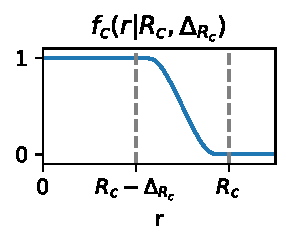
\includegraphics[width=\columnwidth]{figures/cutoff_single.pdf}
  \caption{A smooth radial cutoff suppresses a neighbor contribution as its
  distance approaches the outer cutoff $r_{\mathrm c}$. Smooth decay is needed
  for continuous energies, forces, and Hessians. Figure from the PET paper
  \cite{pet}.}
  \label{fig:cutoff-single}
\end{figure}

\begin{figure}[t]
  \centering
  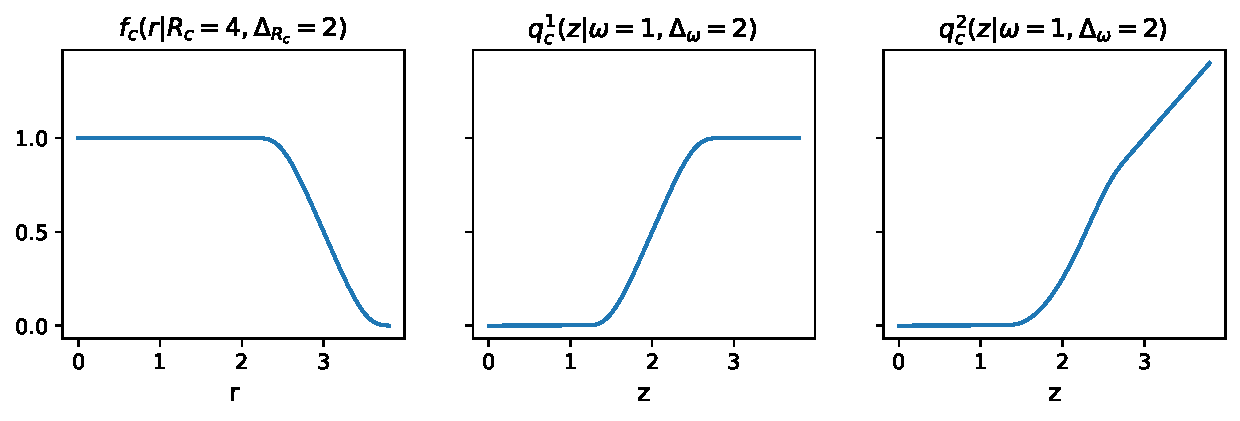
\includegraphics[width=\columnwidth]{figures/cutoff_functions.pdf}
  \caption{Comparison of radial cutoff functions used to attenuate neighbor
  contributions near $r_{\mathrm c}$. The value and the derivatives relevant
  to the model must be treated consistently in every energy contribution.
  Figure from the PET paper \cite{pet}.}
  \label{fig:cutoff-functions}
\end{figure}

Neural networks operate on fixed-width numerical representations. Chemical
identity is therefore mapped from a discrete species label to a trainable
embedding vector,
\begin{equation}
  \bm x_u^{(0)}=\bm E_Z[Z_u]\in\mathbb R^d,
  \label{eq:species-embedding}
\end{equation}
where each row of the embedding matrix $\bm E_Z$ is learned during training.
In the attributed-graph notation, geometry is carried by edge features. For
example, a radial edge signal can be written
\begin{equation}
  \bm x_{uv\bm n}^{\mathrm{edge}}
  =f_{\mathrm c}(r_{uv\bm n})
   \bigl[\varphi_1(r_{uv\bm n}),\ldots,
          \varphi_K(r_{uv\bm n})\bigr],
  \label{eq:radial-embedding}
\end{equation}
and, in models that retain directional information, by the displacement
$\bm r_{uv\bm n}$, its unit vector, spherical harmonics, or learned functions of
these quantities. Here ``embedding vector'' means a vector in latent feature
space; it need not transform as a physical three-dimensional vector.

Suppressing periodic-image labels for a moment, graph connectivity may also be
represented by an adjacency matrix $\bm A$. A relabeling of the nodes by a
permutation matrix $\bm P$ sends
$(\bm X,\bm A)$ to $(\bm P\bm X,\bm P\bm A\bm P^{\mathrm T})$. The geometric
deep-learning prescription is that a node-wise GNN $F$ be permutation
equivariant, whereas a graph-wise scalar readout $f$ be permutation invariant:
\begin{align}
  F(\bm P\bm X,\bm P\bm A\bm P^{\mathrm T})
    &=\bm P F(\bm X,\bm A),
  \\
  f(\bm P\bm X,\bm P\bm A\bm P^{\mathrm T})
    &=f(\bm X,\bm A).
  \label{eq:graph-permutation}
\end{align}
For an interatomic potential, the first relation applies to node
representations and the second to the total energy. Periodic-image and edge
features must be relabeled consistently with their incident nodes.

\subsubsection{Message passing and many-body representations}

In the notation of Ref.~\cite{bronstein2021}, a message-passing GNN computes a
latent node feature $\bm h_u$ by applying a learnable message function $\psi$
on every incoming edge, combining the messages with a
permutation-invariant aggregation $\bigoplus$, and applying a learnable update
function $\phi$:
\begin{equation}
  \bm h_u
  =\phi\!\left(
      \bm x_u,
      \bigoplus_{(v,\bm n)\in\mathcal N_u}
      \psi\!\left(\bm x_u,\bm x_v,
                   \bm x_{uv\bm n}^{\mathrm{edge}}\right)
    \right).
  \label{eq:message-passing}
\end{equation}
Equation~\eqref{eq:message-passing} extends the book's node-feature equation
by conditioning $\psi$ on the geometric edge feature, as required for an
attributed atomistic graph. A sum is the usual choice for $\bigoplus$, though
means, maxima, and other symmetric multiset functions are possible. For a
deep GNN, take $\bm h_u^{(0)}=\bm x_u^{(0)}$, apply
Eq.~\eqref{eq:message-passing} recursively with layer-specific
$\psi_\ell$ and $\phi_\ell$, and denote each layer's output by
$\bm h_u^{(\ell+1)}$. Although the graph initially contains only pairwise
edges, repeated updates create many-body features: after $L$ layers, an atom
can depend on paths extending up to $L$ graph hops. A shared readout $\rho$
maps the final node features to local energies,
$\varepsilon_u=\rho(\bm h_u^{(L)})$, whose sum gives the invariant extensive
energy in Eq.~\eqref{eq:mlip-energy}.

\subsubsection{Point Edge Transformer architecture}
\label{sec:pet-architecture}

The Point Edge Transformer (PET) introduced by Pozdnyakov and Ceriotti
\cite{pet} is the architecture underlying the later PET-MAD potential
\cite{petmad}. PET preserves a distinct latent message on each directed edge.
For a central atom $i$, its transformer processes the incoming edge messages
together and produces a separate outgoing message for each neighbor. This
avoids compressing the entire neighborhood into a single atom representation
before forming outgoing messages. Attention still performs weighted sums
internally; the distinction is that the edge identities survive the update.

\begin{figure*}[t]
  \centering
  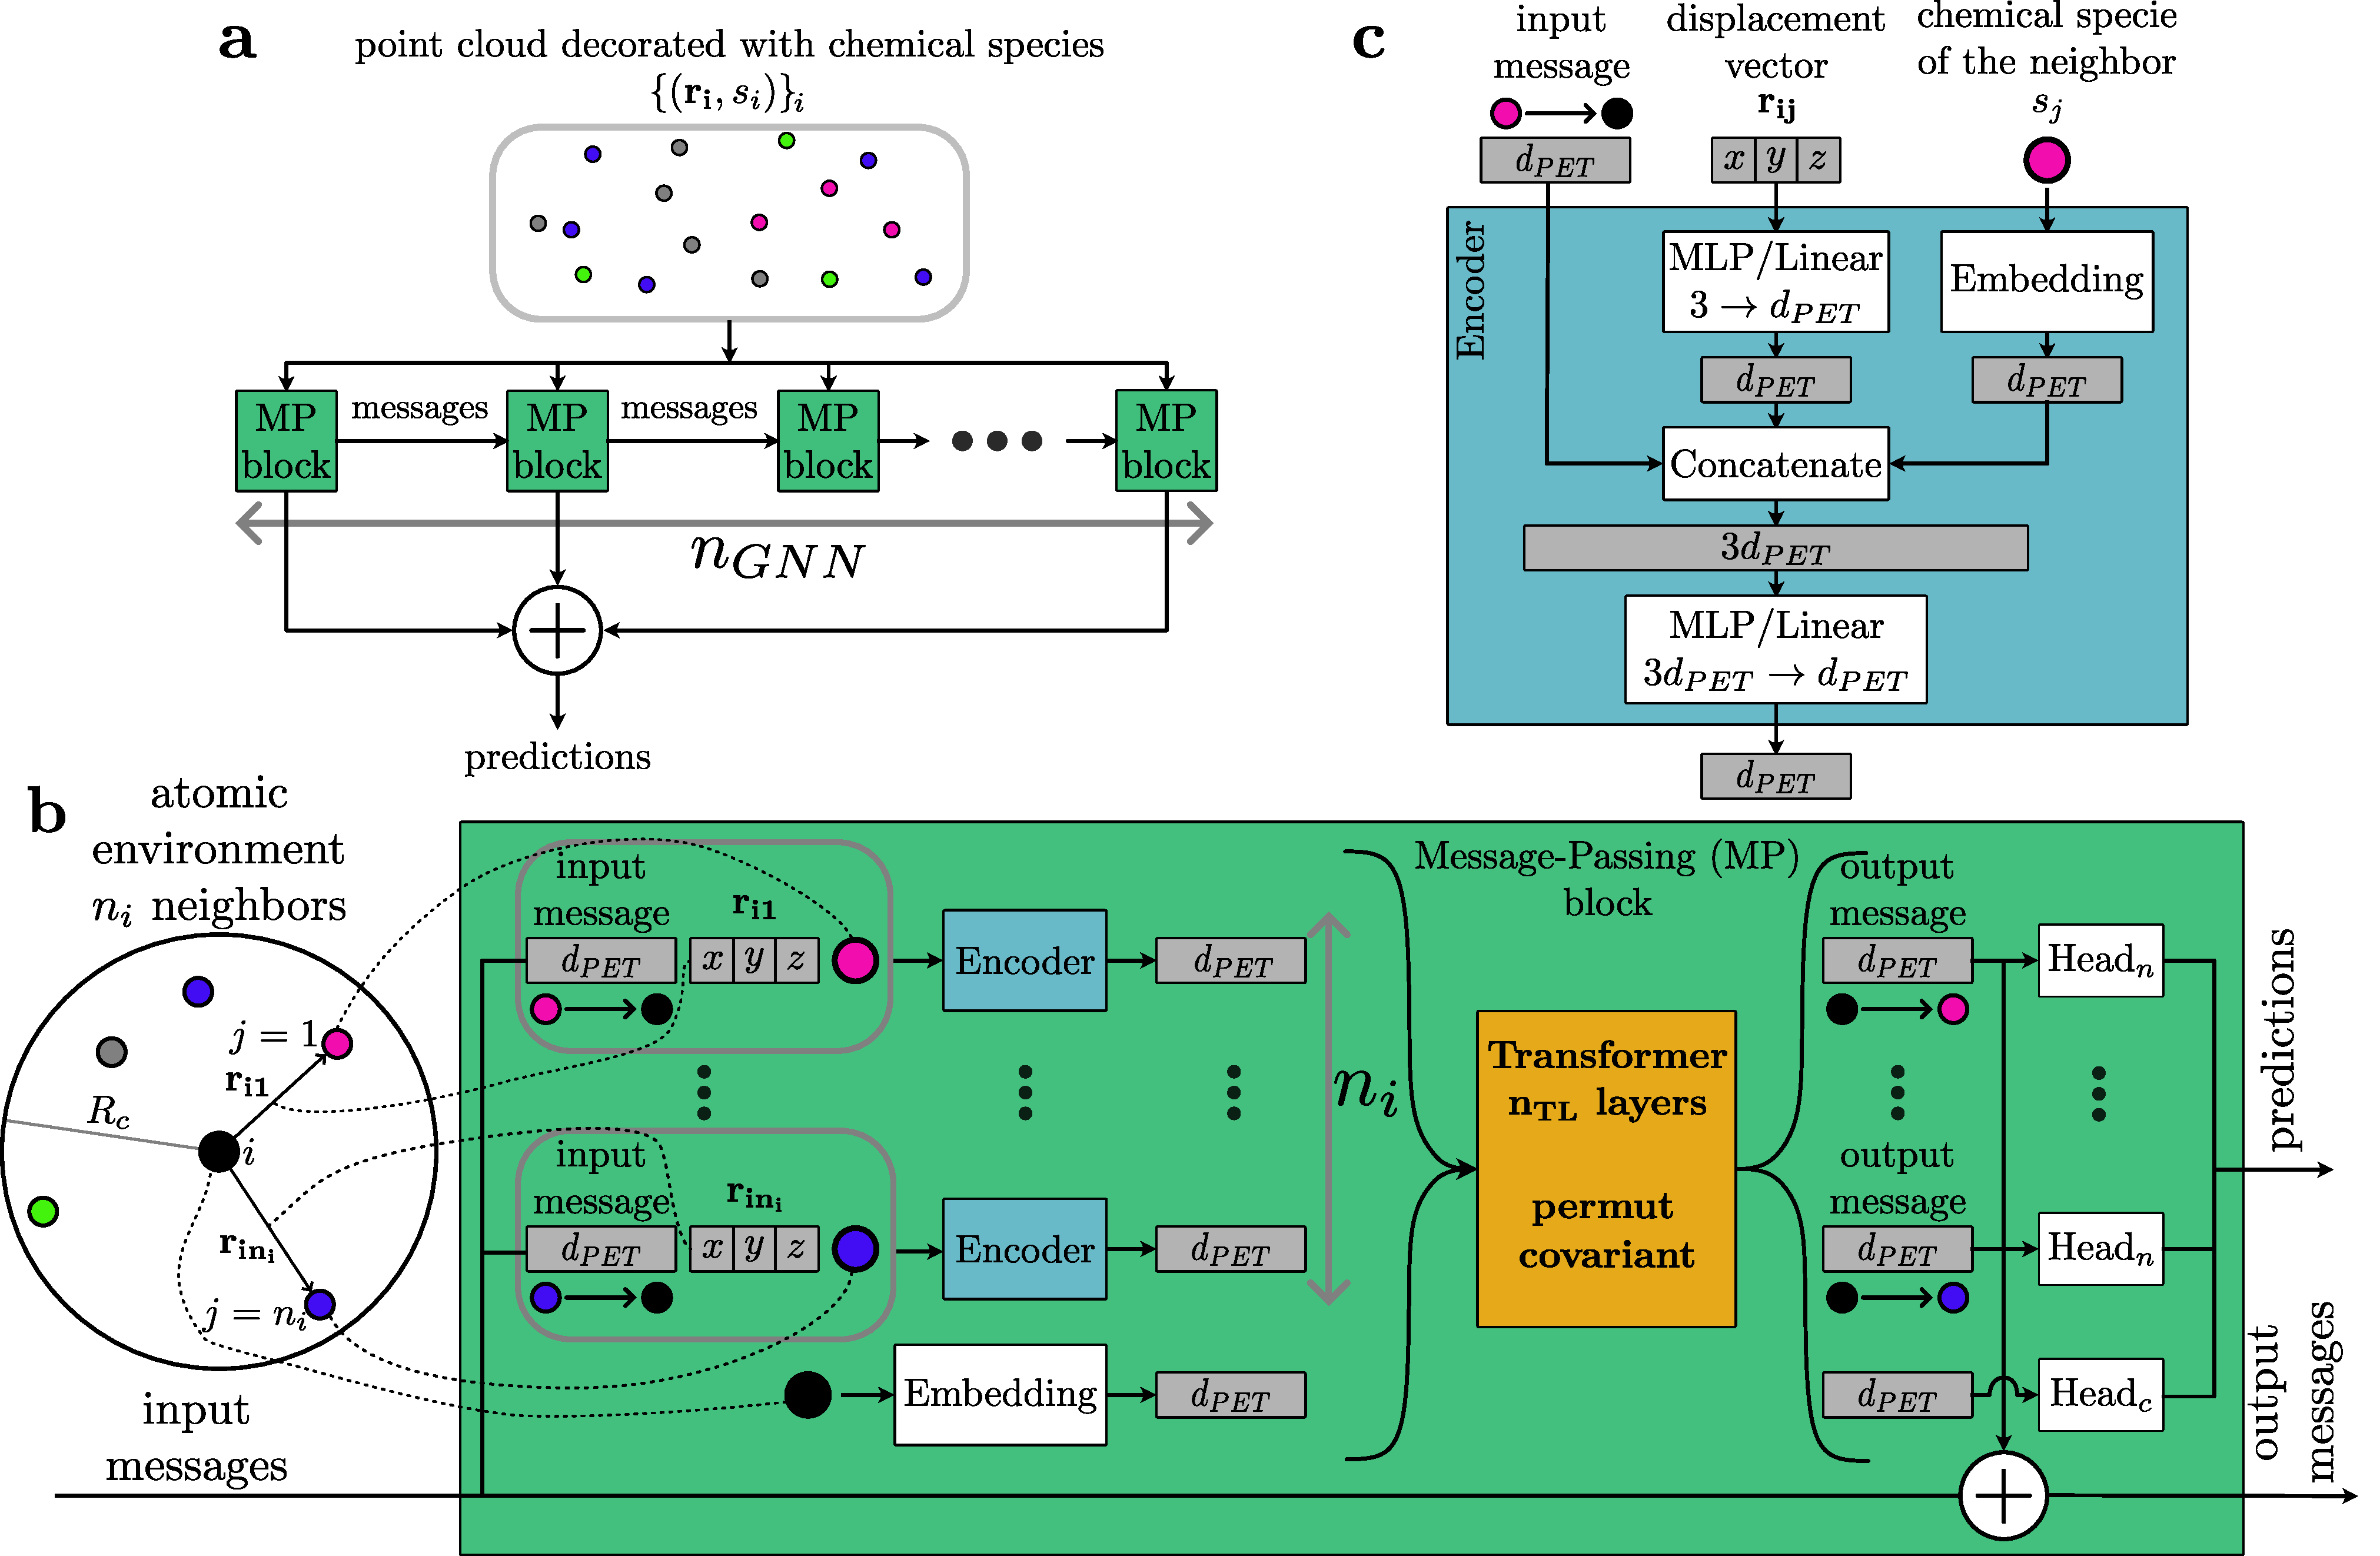
\includegraphics[width=\textwidth]{figures/pet_final.pdf}
  \caption{Point Edge Transformer (PET) message-passing architecture. Edge
  messages associated with a central atom are jointly processed by attention
  while retaining their individual edge identities for the outgoing update.
  Figure from the PET paper \cite{pet}.}
  \label{fig:pet-architecture}
\end{figure*}

In the original formulation (Ref.~\cite{pet}, Appendix A), neighbor species,
relative Cartesian position, and an incoming message
$\bm m_{j\to i}^{(\ell-1)}\in\mathbb R^{d_{\mathrm{PET}}}$ are encoded as
\begin{align}
  \bm p_{ij}^{(\ell)}
    &=\operatorname{SiLU}\bigl(\bm W_r^{(\ell)}\bm r_{ij}
                                      +\bm b_r^{(\ell)}\bigr),
  \\
  \bm t_{ij}^{(\ell)}
    &=\mathrm{MLP}_\ell\!\left(
      \bm m_{j\to i}^{(\ell-1)}\Vert
      \bm E_n^{(\ell)}[Z_j]\Vert
      \bm p_{ij}^{(\ell)}\right),
  \label{eq:pet-token}
\end{align}
where $\Vert$ denotes concatenation. Each ingredient has width
$d_{\mathrm{PET}}$, and the MLP compresses their concatenation from
$3d_{\mathrm{PET}}$ to $d_{\mathrm{PET}}$. In the first block the incoming
message is absent, giving $2d_{\mathrm{PET}}$ input features. A separate
central token, $\bm t_{i0}^{(\ell)}=\bm E_c^{(\ell)}[Z_i]$, uses a distinct
species embedding. These are latent feature vectors with no prescribed
rotation law. Later PET implementations can modify the encoding and feature
dimensions; the project-specific settings are given in
Section~\ref{sec:pet-implementation}.

A transformer mixes the central and neighbor tokens within one environment.
For one attention head, with $a,b$ indexing these tokens,
\begin{align}
  \bm q_a&=\bm W_Q\bm t_a,
  &\bm k_b&=\bm W_K\bm t_b,
  \\
  \bm v_b&=\bm W_V\bm t_b,
  \\
  \alpha_{ab}
    &=\frac{\exp(\bm q_a^{\mathrm T}\bm k_b/\sqrt{d_k})
                    c_b}
            {\sum_c\exp(\bm q_a^{\mathrm T}\bm k_c/\sqrt{d_k})
                    c_c},
  \\
  \bm y_a&=\sum_b\alpha_{ab}\bm v_b.
  \label{eq:self-attention}
\end{align}
where $c_0=1$ for the central token and $c_j=f_{\mathrm c}(r_{ij})$ for
neighbor $j$. The cutoff enters before normalization, so a departing neighbor
vanishes smoothly from both the weighted sum and its denominator.
Multi-head attention repeats this operation in learned subspaces, followed
by feed-forward layers and residual connections. No arbitrary neighbor order
enters the calculation, so permuting neighbors permutes their output tokens
consistently.

Attention makes each neighbor token depend on the other neighbors, allowing
many-body interactions within a single message-passing block. Adding
attention layers increases local expressive power without extending that
block's neighborhood. Adding message-passing blocks communicates information
between environments and enlarges the receptive field. These are separate
architecture choices: the water benchmark in Ref.~\cite{pet} shows that
deeper local transformers can outperform a larger number of shallow
message-passing blocks at fixed total attention-layer count. Local attention
is quadratic in the number of tokens per environment, while the total cost
remains approximately linear in atom count for a fixed architecture and
bounded neighborhood size.

The output neighbor tokens supply outgoing messages, updated with residual
connections to preceding messages. Each block also contributes to the energy.
For the summed-edge variant in the original paper,
\begin{equation}
  \begin{aligned}
  U_\theta={}&\sum_i b_{Z_i}
  +\sum_{\ell=1}^{L}\sum_i\Bigl[
      H_c^{(\ell)}(\bm x_{i0}^{(\ell)})
  \\[-0.2em]
  &+\sum_{j\in\mathcal N_i}f_{\mathrm c}(r_{ij})
                 H_n^{(\ell)}(\bm x_{ij}^{(\ell)})\Bigr],
  \end{aligned}
  \label{eq:pet-readout}
\end{equation}
where $\bm x_{i0}$ and $\bm x_{ij}$ are central and neighbor output tokens,
$H_c$ and $H_n$ are learned readout heads, and $b_Z$ are fitted species
baselines. Appendix A of Ref.~\cite{pet} also describes a cutoff-weighted
average of edge predictions. The edge terms are many-body learned
contributions, not physical pair energies. Contributions from all blocks
enter the total, and cutoff weighting is required in the readout as well as
in attention.

\subsubsection{Physical symmetries}

For an isolated non-magnetic system without external fields, a valid scalar
energy should be unchanged by translation, rotation or reflection of the
whole structure and by permutation of identical atoms:
\begin{equation}
  \begin{aligned}
  U(\bm R)&=U(\bm R+\bm a)=U(\bm Q\bm R)
  \\
           &=U(\bm P\bm R),\qquad \bm Q\in O(3).
  \end{aligned}
  \label{eq:energy-symmetry}
\end{equation}
An invariant scalar is unchanged by a symmetry operation, whereas an
equivariant vector changes in the corresponding way; for example,
$\bm F_i(\bm Q\bm R)=\bm Q\bm F_i(\bm R)$. Translation invariance follows
from using relative positions, and the shared local functions and symmetric
aggregation enforce permutation invariance. Many MLIPs impose rotational
symmetry exactly through invariant geometric descriptors or
$E(3)$-equivariant features. PET instead processes Cartesian displacement
vectors with an unconstrained transformer and learns rotational behavior from
random rotational augmentation \cite{pet,petmad}. Thus the PET-MAD backbone
is not intrinsically exactly rotation invariant. The PET-MAD publication
reports rotational discrepancies usually smaller than its prediction errors
\cite{petmad}; this is not a validation of the particular MOF-5 structures or
checkpoint used here. For periodic structures, rotation tests must rotate
both positions and cell vectors.

\subsubsection{Exact rotational symmetrization with ECSE}

The original PET paper also introduces the Equivariant Coordinate System
Ensemble (ECSE), a separate construction that imposes exact rotational
symmetry on a smooth, translation- and permutation-invariant backbone
\cite{pet}. Each ordered noncollinear neighbor pair $(j,k)$ defines a local
frame $\bm Q_{ijk}$ that rotates with the atomic environment. For a scalar
local prediction, the symmetrized model is

\begin{figure*}[t]
  \centering
  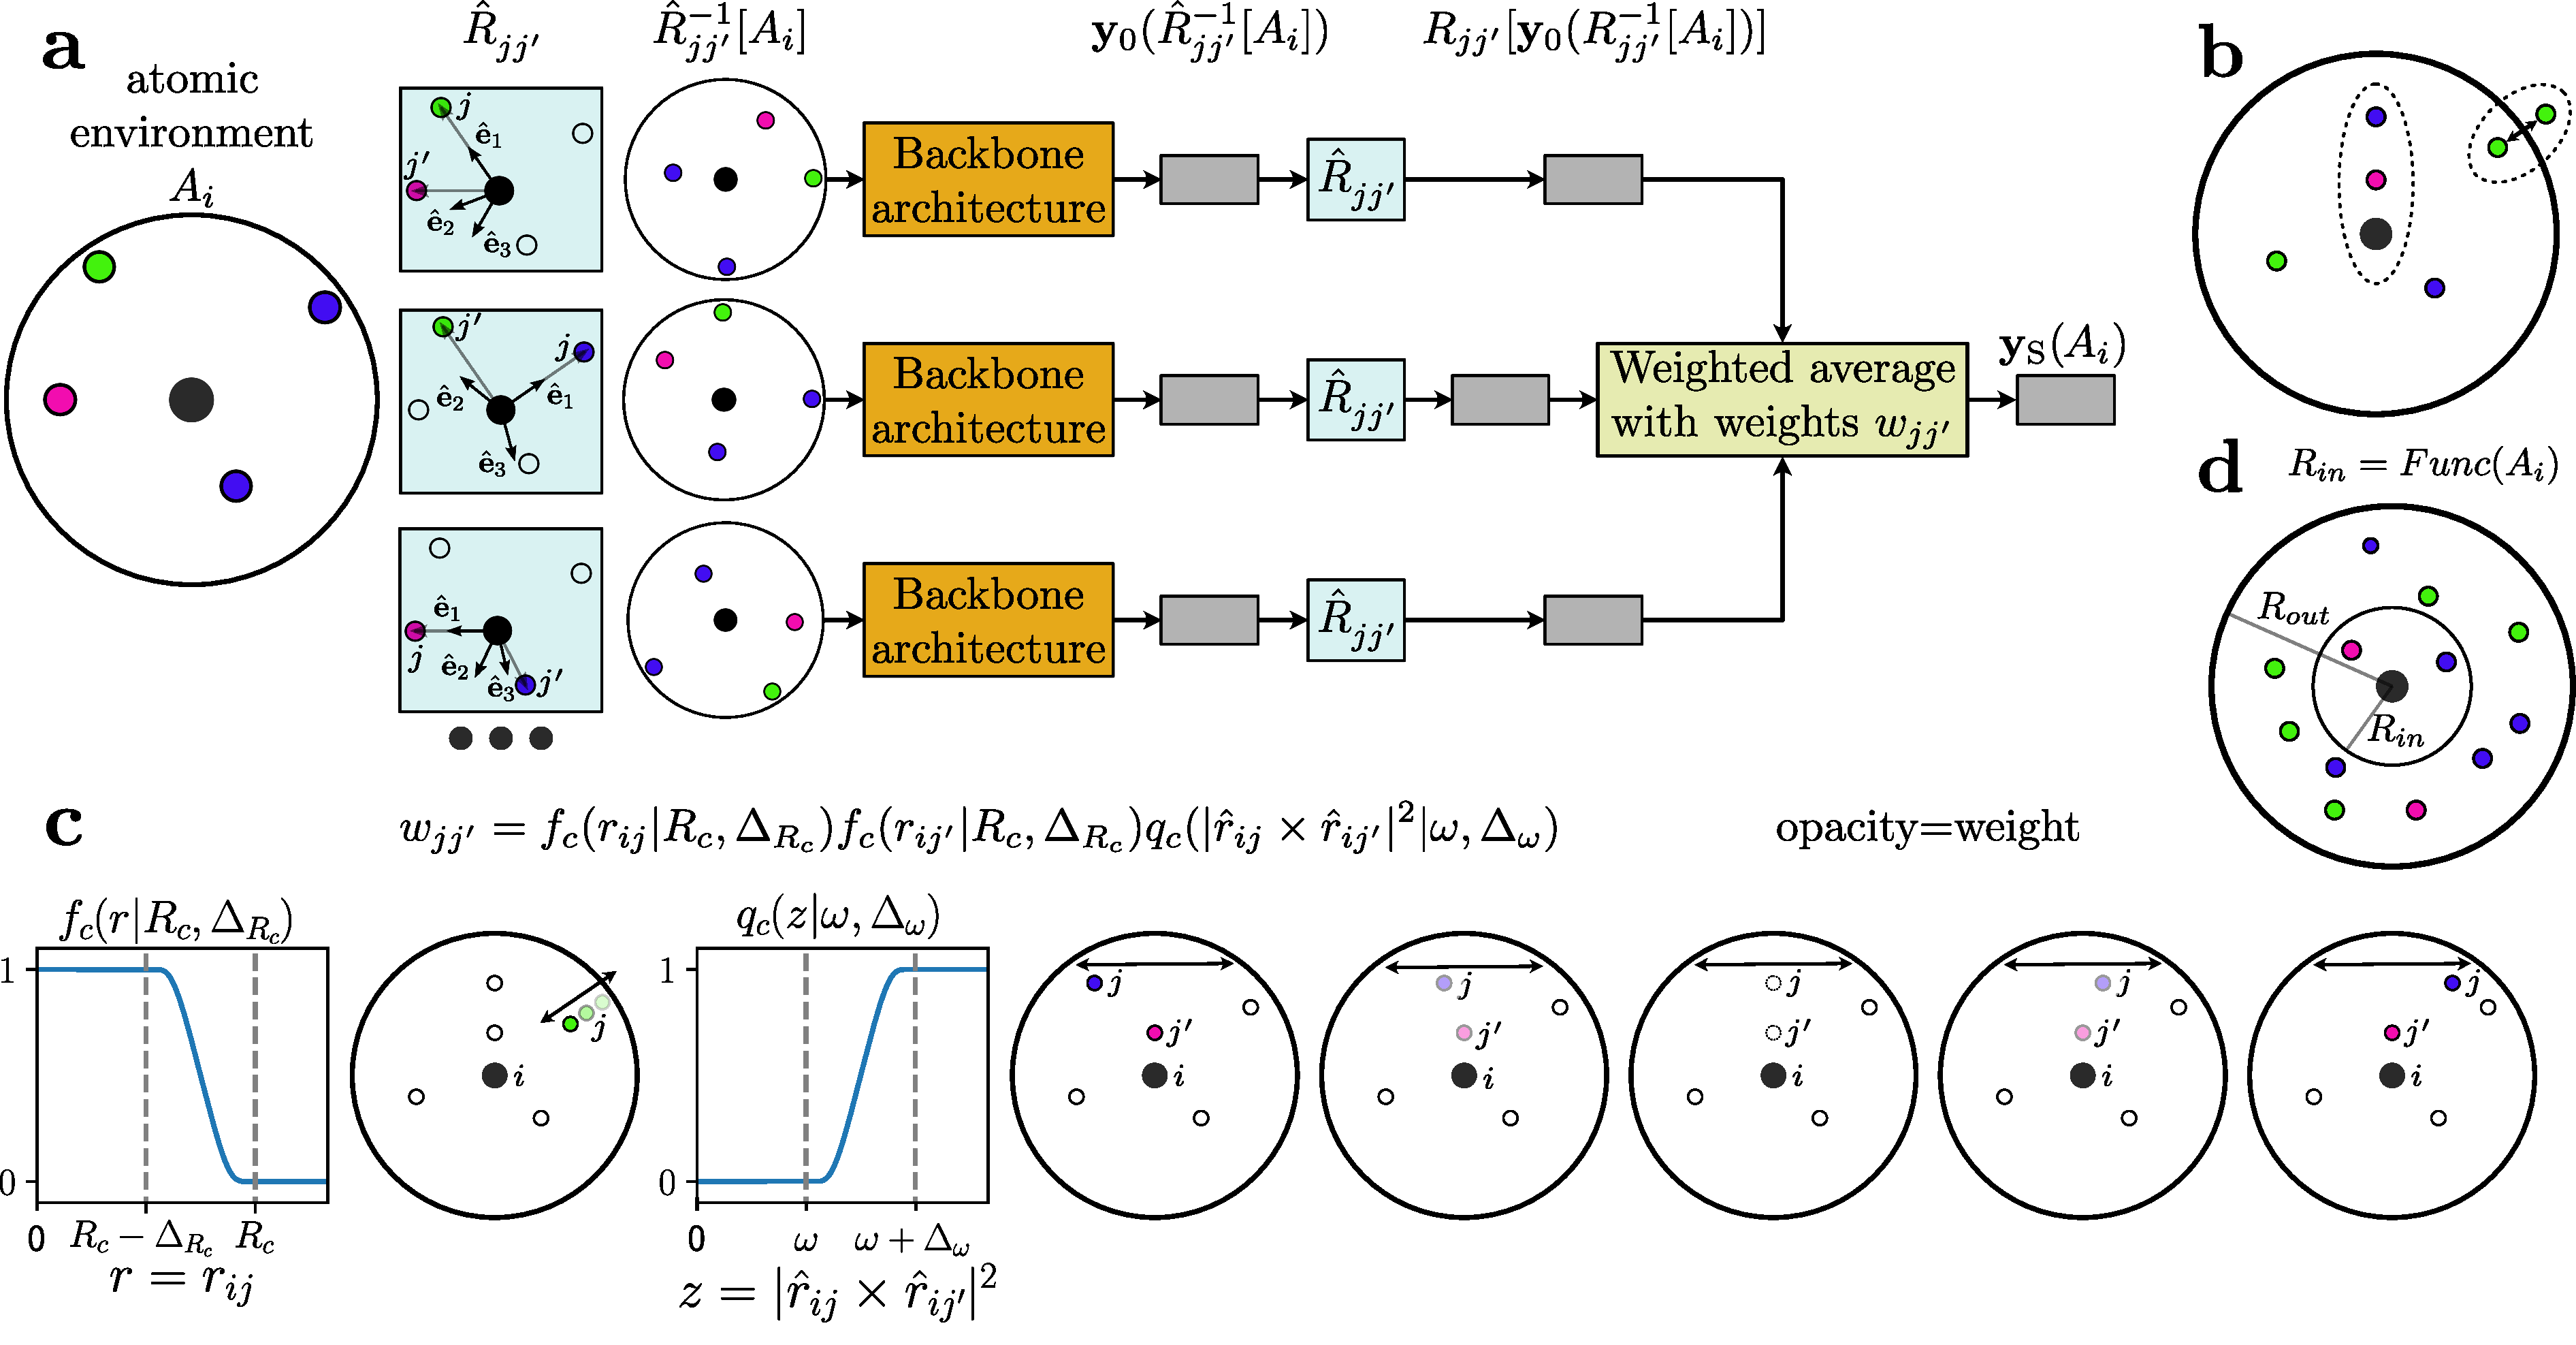
\includegraphics[width=\textwidth]{figures/ecse_final.pdf}
  \caption{Equivariant Coordinate System Ensemble (ECSE). Local coordinate
  frames constructed from noncollinear neighbor pairs rotate with the atomic
  environment; predictions evaluated in these frames are transformed as
  needed and smoothly averaged. Figure from the PET paper \cite{pet}.}
  \label{fig:ecse}
\end{figure*}

\begin{equation}
  \varepsilon_i^{\mathrm{ECSE}}=
    \frac{\sum_{j\ne k}w_{ijk}\,
          \varepsilon_i^0(\bm Q_{ijk}^{\mathrm T}\mathcal N_i)}
         {\sum_{j\ne k}w_{ijk}},
  \label{eq:ecse}
\end{equation}
where the notation indicates expressing all relevant displacement vectors in
that frame. Vector or tensor predictions are transformed back to the
original frame before averaging. The frames in the paper use proper
rotations, $SO(3)$; reflection invariance in Eq.~\eqref{eq:energy-symmetry}
is an additional requirement, not a consequence of this construction alone.

Radial weights suppress frames whose defining neighbors approach the cutoff,
and angular weights suppress nearly collinear pairs. An adaptive inner radius
and smooth pruning reduce the number of frames. Fully collinear environments
require a fallback; the paper demonstrates an auxiliary invariant model.
Using a smooth ensemble avoids the discontinuities caused by selecting only
the two nearest neighbors. This frame-selection radius is distinct from the
adaptive neighbor cutoff in the later PET implementation used here.

Forces and Hessians must differentiate the full expression in
Eq.~\eqref{eq:ecse}, including the position dependence of frames and weights.
They cannot be obtained simply by averaging derivatives of the backbone.
The paper shows that tight frame-selection parameters can amplify derivative
errors even when the energy remains mathematically smooth. Its
proof-of-principle ECSE implementation incurs roughly three orders of
magnitude of inference overhead (Ref.~\cite{pet}, Section 6 and Appendix F).
ECSE is not enabled in this project's workflow; its exact symmetry properties
must therefore be distinguished from those of the deployed PET backbone.

\subsubsection{Training and domain of validity}

Given reference configurations $s$, a typical energy--force training
objective is
\begin{equation}
  \begin{aligned}
  \mathcal L(\theta)=\sum_s\Biggl[{}
    w_E\left(\frac{U_\theta^{(s)}-U_{\mathrm{ref}}^{(s)}}{N_s}\right)^2
  \\
    +\frac{w_F}{3N_s}\sum_{i\alpha}
      \left(F_{i\alpha,\theta}^{(s)}
                 -F_{i\alpha,\mathrm{ref}}^{(s)}\right)^2
  \Biggr],
  \end{aligned}
  \label{eq:mlip-loss}
\end{equation}
possibly augmented by stress terms and regularization. Because the force
labels are derivatives of the PES, each configuration supplies $3N_s$ local
slope constraints in addition to its energy. Optimization adjusts the
embeddings, message-passing transformations and readout weights to minimize
this loss. The original PET experiments first subtract fitted species
baselines and use a loss that rescales energy and force errors by moving
validation-set mean squared errors, together with Adam and random rotational
augmentation (Ref.~\cite{pet}, Appendix B). Equation~\eqref{eq:mlip-loss}
is a generic objective, not that paper's exact normalization. PET-MAD was
trained on a chemically diverse DFT dataset rather than
on MOF-5 alone, making it a universal pretrained potential \cite{petmad}.

An MLIP interpolates the reference PES represented by its training data; it
does not replace the approximations of the underlying electronic-structure
method and need not extrapolate reliably to unfamiliar bonding, charge states,
very short distances or thermodynamic phases. Energy and force test errors,
trajectory stability and uncertainty indicators are therefore necessary but
distinct checks. This project also uses second derivatives, which can be more
sensitive than energies or forces and were not directly constrained by the
usual loss in Eq.~\eqref{eq:mlip-loss}. Curvatures and vibrational spectra must
therefore be validated explicitly. The original PET benchmarks include
isolated distorted methane, water, molecular collisions, crystals, and
high-entropy alloys, but do not validate methane adsorption in MOF-5. The
paper also reports weaker high-temperature alloy extrapolation despite strong
hold-out accuracy, illustrating the distinction between expressiveness and
transferability \cite{pet}.

\subsection{Metal--organic frameworks and MOF-5}

\begin{figure}[t]
  \centering
  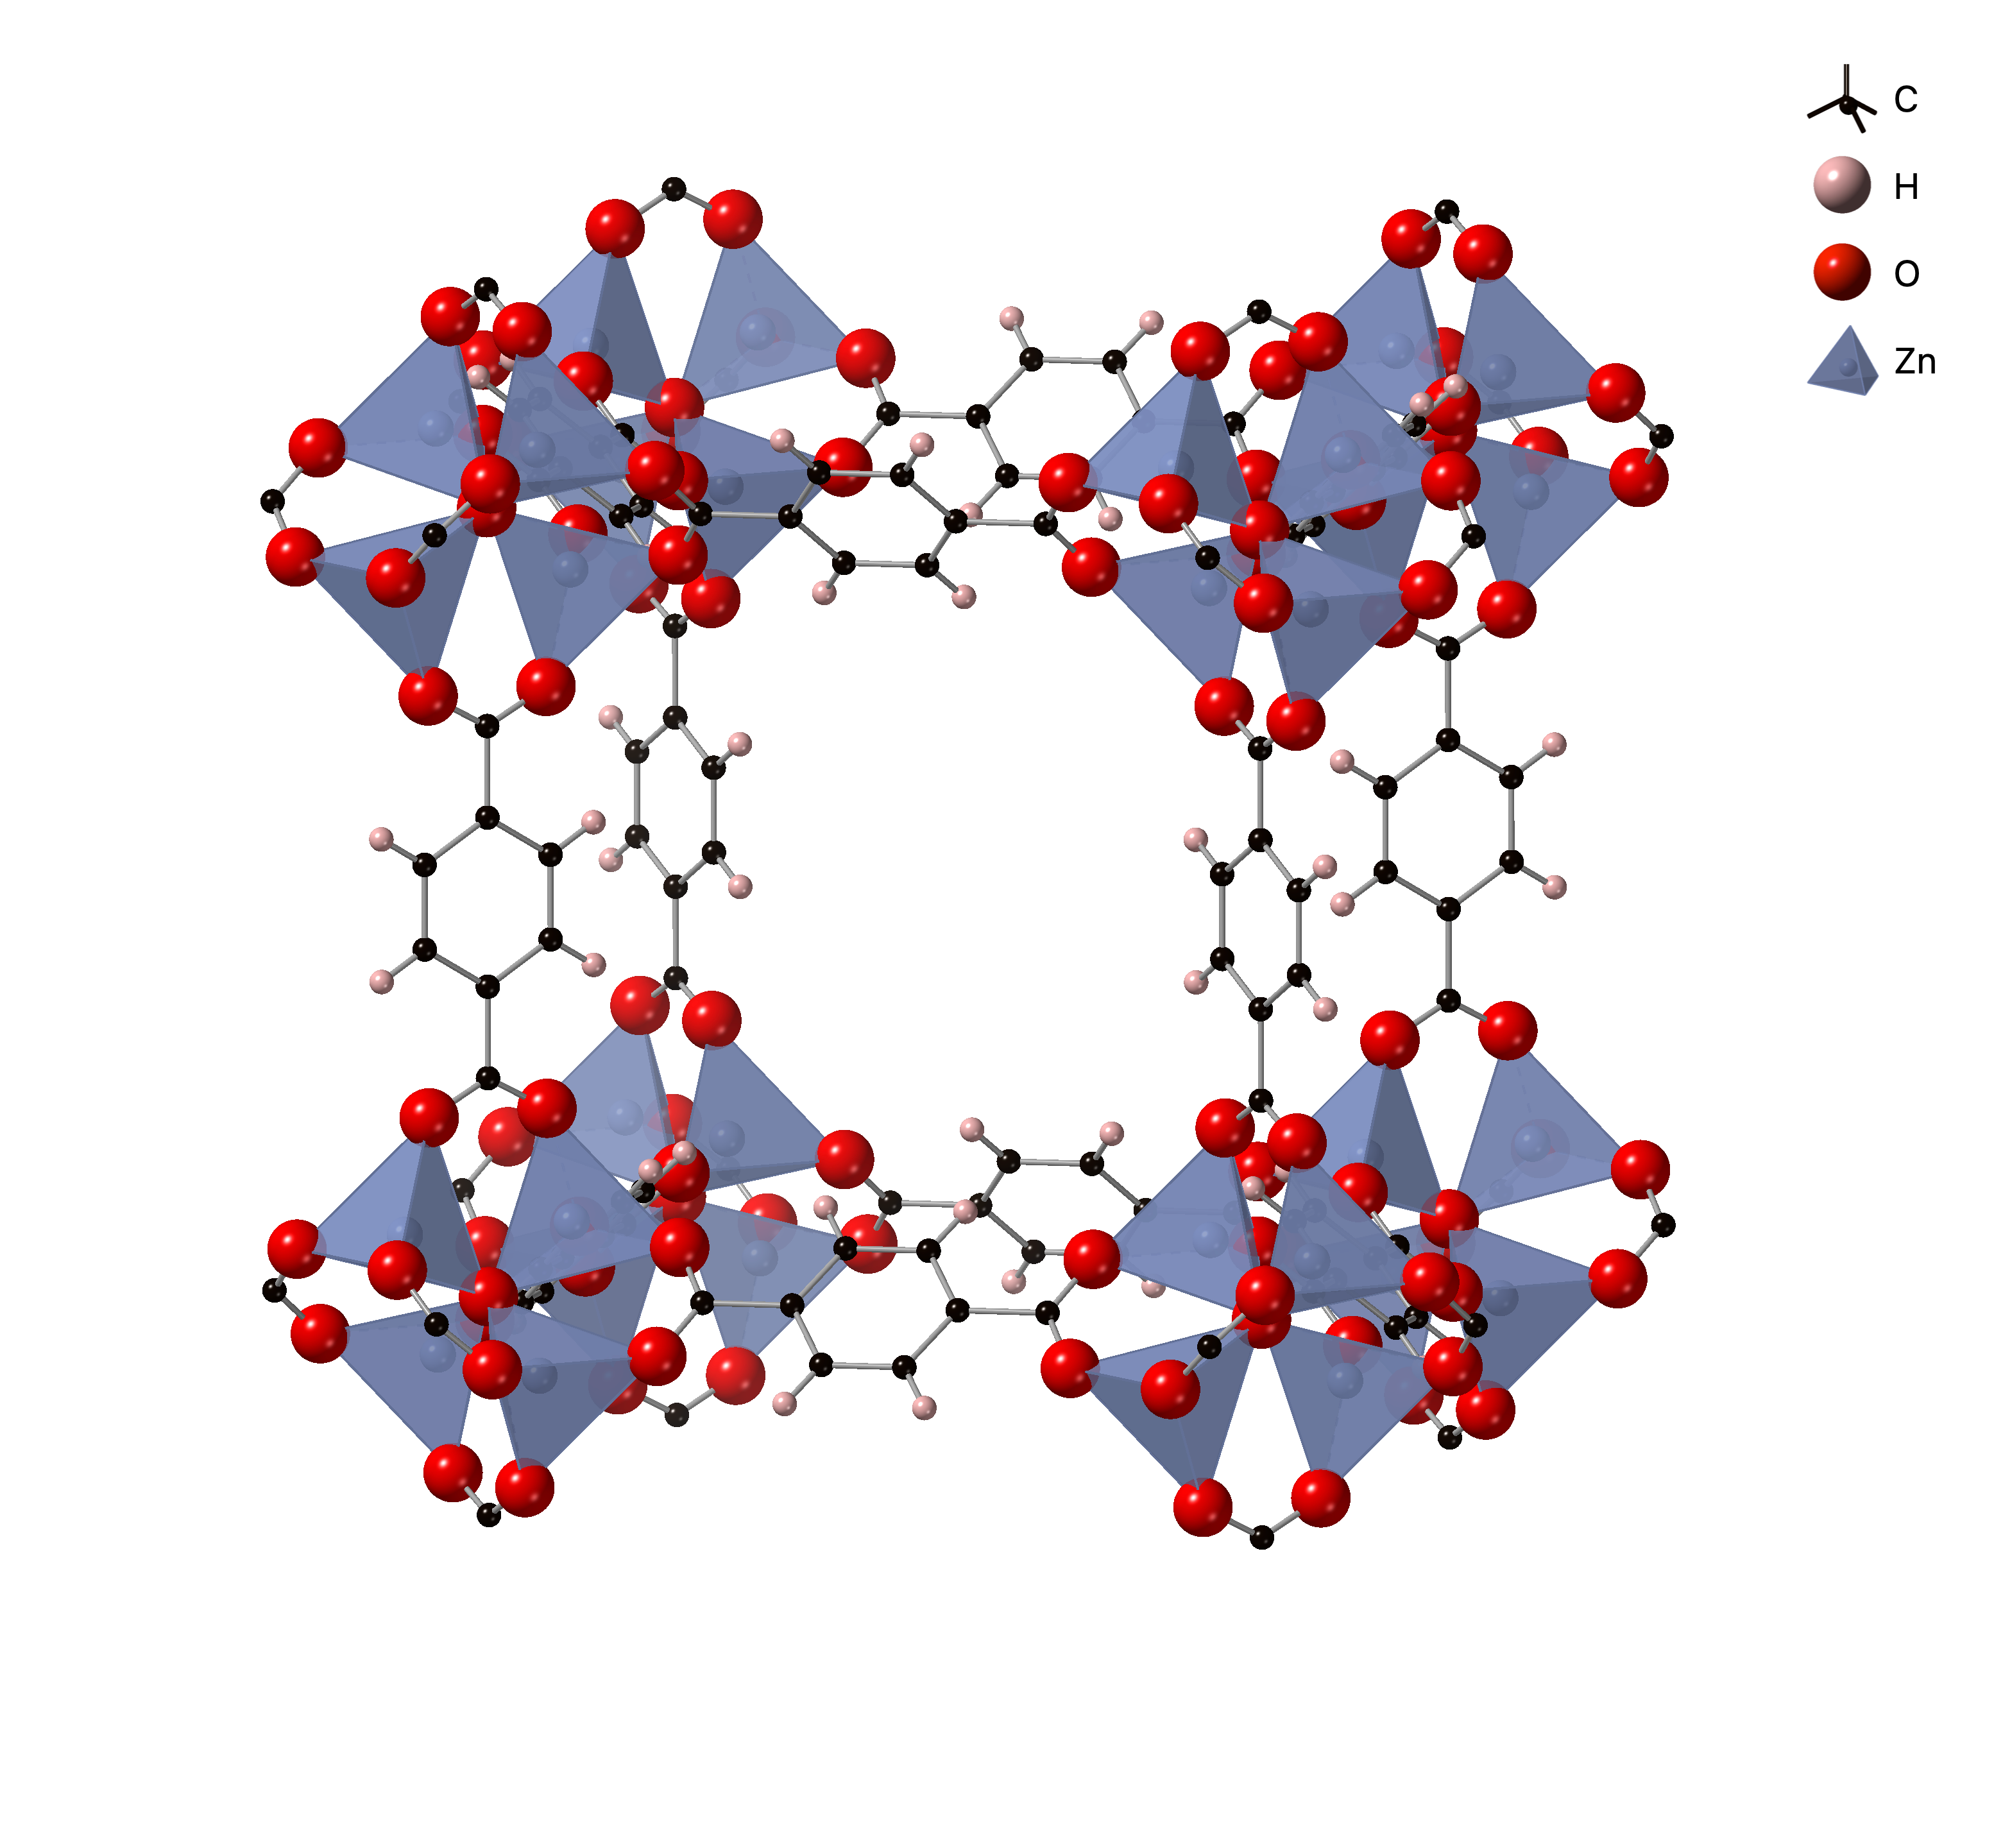
\includegraphics[width=\columnwidth]{figures/mof-5.png}
  \caption{Ball-and-polyhedron representation of the MOF-5 framework. The
  zinc--oxo clusters are shown as blue polyhedra, connected by
  benzene-1,4-dicarboxylate linkers. The legend identifies carbon (black),
  hydrogen (pink), oxygen (red), and zinc (blue). The open spaces between
  framework components form the pores that host adsorbed molecules.}
  \label{fig:mof5}
\end{figure}

Metal--organic frameworks are crystalline networks assembled from metal ions
or metal--oxo clusters joined by organic molecules called linkers. The
connections repeat in three dimensions and leave accessible pores between
them. Changing the nodes and linkers can alter the pore size, surface
chemistry, and framework flexibility. This makes MOFs useful for studying gas
storage and separation: guest molecules can enter the pores and adsorb on
their internal surfaces without becoming part of the framework.

MOF-5 provides a concrete example (Figure~\ref{fig:mof5}). Zinc--oxo clusters
are connected by benzene-1,4-dicarboxylate linkers to form an open, periodic
framework. Methane occupies its pores and interacts with the framework mainly
through weak noncovalent forces. At a given temperature and loading, the methane molecules
can move among adsorption environments, while the linkers and clusters also
vibrate. The framework therefore supplies both the space that holds the gas
and the flexible surroundings that influence its motion.

These motions explain why heat capacity is an informative property for this
project. Heating excites framework vibrations and methane's internal modes,
but also changes how methane explores the pores and interacts with the host.
The latter effects can be anharmonic and cannot be inferred from vibrations
about a single structure \cite{kapil2019}. We therefore use classical MD of
\emph{loaded} MOF-5 to sample the temperature-dependent host--guest motion,
and normal modes of optimized loaded structures to correct the classical
treatment of quantized vibrations. An empty MOF-5 Hessian provides a framework
reference; the loaded-system Hessian supplies the correction used for the
reported loaded-system heat capacity.

\subsection{Thermodynamic definitions}

\subsubsection{Heat-capacity estimators used in this report}

Section~\ref{sec:md-response} derives the thermodynamic definitions and
fluctuation formulas for $C_V$ and $C_P$. The present workflow obtains the
classical constant-pressure term by differentiating replica-averaged physical
enthalpies $\langle H\rangle=\langle E+P_{\mathrm{ext}}V\rangle$ on a temperature
grid. The ensemble, loading, and external pressure are held fixed across that
grid, and uncertainty is propagated through the differentiation. Equilibrated
NPT enthalpy fluctuations provide an independent consistency check when
sampling is sufficient.

The quantum correction is evaluated separately from harmonic normal-mode
frequencies. It is formally a $C_V$ correction, whereas the trajectory term is
$C_P$. Equation~\eqref{eq:cp-cv} explains why adding these terms requires the
pressure--volume contribution to the quantum correction to be small; the two
heat capacities are not interchangeable by definition. Extensive cell heat
capacities are combined before division by the total loaded-cell mass.

\subsubsection{LLPR model uncertainty and CEA propagation}
\label{sec:llpr-cea}

The uncertainty of a machine-learned potential is different from the sampling
error of a finite MD trajectory. This project estimates the former for the
classical NPT term and harmonic correction with a persistent last-layer
prediction-rigidity (LLPR) ensemble
\cite{bigi2024}, and the latter with autocorrelation-aware statistics and
independent replicas. These quantities are kept separate throughout the
analysis.

For a fixed trained representation, write the central PET energy as
$\bar U(\bm x)=\bm w_0^{\mathrm T}\bm f(\bm x)$, where $\bm f$ is the
last-layer feature vector. If $\bm F$ contains the corresponding features of a
reference-labeled covariance set, the metatrain LLPR standard deviation has
the form
\begin{equation}
  \begin{aligned}
  \sigma_{\mathrm{LLPR}}^2(\bm x)
  ={}&\alpha^2\bm f(\bm x)^{\mathrm T}
  \\
  &\times\left(\bm F^{\mathrm T}\bm F
        +\lambda\bm I\right)^{-1}\bm f(\bm x).
  \end{aligned}
  \label{eq:llpr-variance}
\end{equation}
The regularizer $\lambda$ stabilizes weakly constrained feature directions.
The scale $\alpha$ is fitted against energy residuals on a separate,
reference-labeled calibration set. The two sets must be disjoint and use the
same electronic-structure definition as the base potential. Model predictions
cannot serve as reference labels for calibrating their own errors.

Equation~\eqref{eq:llpr-variance} is exported as
\texttt{energy\_uncertainty}, a standard deviation in energy units. That
scalar is useful for calibration and out-of-domain diagnostics but cannot be
propagated through an equilibrium average by itself. The propagation needs
signed, correlated changes in energy across configurations. Metatrain
therefore samples persistent shallow readout weights,
\begin{equation}
  \begin{aligned}
  \bm w_i&\sim\mathcal N\!\left[
    \bm w_0,
    \alpha^2\left(\bm F^{\mathrm T}\bm F
                         +\lambda\bm I\right)^{-1}\right],
  \\
  U^{(i)}(\bm x)&=\bm w_i^{\mathrm T}\bm f(\bm x),
  \end{aligned}
  \label{eq:llpr-members}
\end{equation}
and exports their energies as \texttt{energy\_ensemble}. In the large-member
limit, their framewise standard deviation approaches the analytical LLPR
standard deviation. This is a shallow ensemble: the learned representation is
fixed, so it cannot reveal a model bias or representation error shared by all
members and should not be described as a committee of independently trained
neural networks.

The ensemble is propagated using the reweighting framework of Imbalzano
\emph{et al.}\ \cite{imbalzano2021}. On a production frame $t$ sampled by the
central model at temperature $T$, define
\begin{align}
  \Delta U_t^{(i)} &= U_t^{(i)}-\bar U_t,\\
  H_t^{(i)} &= K_t+U_t^{(i)}+P_{\mathrm{ext}}V_t,
  \label{eq:llpr-frame-enthalpy}
\end{align}
where $K_t$ and cell volume $V_t$ come from the central NPT
trajectory. Normalized exponential reweighting gives
\begin{equation}
  \left\langle H^{(i)}\right\rangle_i^{\mathrm{direct}}
  =\frac{\sum_t e^{-\beta\Delta U_t^{(i)}}H_t^{(i)}}
  {\sum_t e^{-\beta\Delta U_t^{(i)}}},
  \label{eq:llpr-direct}
\end{equation}
but can collapse when the energy difference is extensive. The primary
large-system estimate is therefore the first-order cumulant expansion
approximation (CEA),
\begin{equation}
  \begin{aligned}
  \left\langle H^{(i)}\right\rangle_i^{\mathrm{CEA}}
  ={}&\left\langle H^{(i)}\right\rangle_{\bar U}
  \\
  &-\beta\operatorname{cov}_{\bar U}
  \left(H^{(i)},\Delta U^{(i)}\right),
  \\
  &\beta=(k_{\mathrm B}T)^{-1}.
  \end{aligned}
  \label{eq:llpr-cea}
\end{equation}
Direct reweighting is retained as a diagnostic. Its member-wise effective
sample count $N_{\mathrm{eff}}=1/\sum_t\widetilde w_t^2$ detects weight
collapse. The additional diagnostic
$\operatorname{var}_{t}(\beta\Delta U_t^{(i)})$ should be much smaller than
one for a controlled first-order CEA. A large value warns that omitted
higher-order terms may be important; agreement with direct reweighting is
meaningful only where $N_{\mathrm{eff}}$ remains adequate.

At each temperature, independent replicas are averaged member by member. The
same exported ensemble and member index must be used at every temperature.
The analysis then differentiates each complete enthalpy curve,
\begin{equation}
  \begin{aligned}
  C_{P,\mathrm{cl}}^{(i)}(T)
  &=\frac{\mathrm d\langle H^{(i)}\rangle_i^{\mathrm{CEA}}}
          {\mathrm dT},
  \\
  \sigma_{\mathrm{LLPR},C_P}(T)
  &=\left\{\frac{1}{M-1}\sum_{i=1}^{M}
  \left[C_{P,\mathrm{cl}}^{(i)}(T)
  -\overline C_{P,\mathrm{cl}}(T)\right]^2\right\}^{1/2}.
  \end{aligned}
  \label{eq:llpr-cp-spread}
\end{equation}
The reported LLPR error is therefore the sample standard deviation of the
final member-resolved $C_P$ curves. It is not the instantaneous energy spread,
and it is not divided by $\sqrt M$: ensemble members sample a predictive
distribution rather than provide repeated measurements of one mean.

\subsubsection{Gaussian NPT propagation of shallow-ensemble uncertainty}
\label{sec:gaussian-propagation}

Direct propagation of shallow ensembles (DPOSE) carries persistent model
members through a property calculation before taking their spread
\cite{kellner2024}. The saved comparison uses a project-specific Gaussian NPT
approximation, rather than separate trajectories under each member. Define
$Q_i=U_i+P_{\mathrm{ext}}V$ and $\Delta U_i=U_i-U_0$, where subscript 0
identifies the central potential. If $(Q_i,\Delta U_i)$ is jointly Gaussian,
exponential reweighting shifts its mean but leaves its covariance unchanged.
Integrating out separable quadratic momenta then gives
\begin{equation}
 C_{P,i}^{\mathrm G}\simeq\frac{f}{2}k_{\mathrm B}
       +\frac{\operatorname{var}_0(Q_i)}{k_{\mathrm B}T^2}.
 \label{eq:gaussian-member-cp}
\end{equation}
The variance is measured on the central trajectory, not a member-equilibrated
trajectory. The Gaussian assumption makes that substitution possible; it is
not needed for the exact central-model fluctuation estimator in
Section~\ref{sec:md-response}. Here $f=3N-3$, and extensive results are divided
by the loaded-cell mass. Member indices must remain paired when adding the
harmonic corrections so that classical--harmonic covariance is retained.

Two comparisons must be distinguished. The main Gaussian/DPOSE plots retain
the central enthalpy-derivative curve and its sampling error, replacing only
the propagated model spread. The separate variance-based hybrid calculation
also replaces the central classical value and estimates its sampling error
from the squared configurational-enthalpy fluctuations. Neither construction
guarantees a smaller band or removes the need to validate sampling and the
Gaussian approximation.

\subsubsection{Why classical and quantum predictions differ}

In the classical harmonic limit, every quadratic vibrational degree of
freedom contributes $k_{\mathrm B}$ to \cv, producing the Dulong--Petit limit
at all temperatures. Quantum mechanically, a mode of angular frequency
$\omega$ becomes thermally populated only when $\hbar\omega$ is comparable to
or smaller than $k_{\mathrm B}T$. High-frequency framework and molecular modes
are therefore partially frozen near room temperature. Classical MD can still
describe anharmonic structural motion, but it cannot generate the correct
quantum populations simply by extending the trajectory.

\section{Reference evidence and the hybrid approximation}

Kapil \emph{et al.}\ studied empty MOF-5 and cells containing 50, 100, and
150 methane molecules \cite{kapil2019}. Their results establish the physical
motivation for combining a classical anharmonic term with a harmonic quantum
correction, and test that approximation for their force field. This project
uses the hybrid method as a computational strategy for PET, rather than as a
recipe for reproducing their numerical results.

\subsection{Differences from the reference calculation}
\label{sec:reference-comparison}

The reference work used analytical QuickFF force fields derived from
electronic-structure calculations, not PET-MAD \cite{quickff}. Framework
covalent terms were
fitted to B3LYP cluster calculations, with MBIS charges obtained from a
periodic PBE density. Nonbonded interactions combined Gaussian-distributed
electrostatics with an MM3 Buckingham model and a \SI{15}{\angstrom} cutoff
with tail corrections. Methane was inserted with RASPA, configurations with
unrealistic contacts were rejected, and canonical Monte Carlo was used before
dynamics. The present workflow instead uses PET for all energy, force, and
Hessian evaluations, and independently generated loaded configurations.
These differences are expected and are not defects to be removed by matching
individual reference parameters.

The reference heat-capacity curves were evaluated from neighboring enthalpies,
\begin{equation}
  \begin{aligned}
  C_P(T)&\simeq
  \frac{\langle H\rangle_{T+\Delta T}-\langle H\rangle_{T-\Delta T}}
       {2\Delta T},
  \\
  \Delta T&=\SI{25}{K},
  \end{aligned}
  \label{eq:finite-difference-cp}
\end{equation}
rather than from a single short trajectory. The present classical term uses
the same thermodynamic principle: every temperature point depends on
converged, statistically independent simulations at adjacent temperatures.

For the harmonic comparison, optimized structures were used to construct
Cartesian Hessians with Yaff and normal modes with TAMkin. Empty MOF-5 was
tested with both QuickFF and UFF4MOF. The loaded 100-methane calculation used
five different Monte Carlo configurations, each optimized into a local
minimum before its harmonic spectrum was evaluated.

\subsection{Physical conclusions relevant to this project}
\label{sec:reference-conclusions}

The main findings of the reference study are:

\begin{itemize}
  \item Empty MOF-5 is quantum mechanical but nearly harmonic over the studied
        range. Its quantum harmonic \cv{} is close to the reported \cpheat{},
        with a room-temperature gravimetric value of approximately
        \SI{0.7}{J\per g\per K}.
  \item Classical MD overestimates the empty-framework heat capacity because
        it populates all vibrational modes according to equipartition.
  \item Methane loading introduces strongly anharmonic host--guest motion.
        The reported heat-capacity curves develop a loading-dependent minimum
        around \SI{200}{K}, caused mainly by changes in attractive host--guest
        interactions as confined methane becomes more mobile.
  \item A harmonic calculation cannot represent diffusion, cage-to-cage
        motion, or the temperature-dependent localization of methane. Nuclear
        quantum effects and anharmonic sampling are both needed for a
        quantitative loaded-system \cpheat{}.
  \item The approximate combination
        \begin{equation}
          C \approx C_{\mathrm{qn}}^{\mathrm{har}}
          - C_{\mathrm{cl}}^{\mathrm{har}}
          + C_{\mathrm{cl}}^{\mathrm{anh}}
          \label{eq:quantum-correction}
        \end{equation}
        qualitatively recovers the loaded minimum and becomes useful above
        roughly \SI{200}{K} in their 100-methane test.
\end{itemize}

The operational form used here is Eq.~\eqref{eq:hybrid-cp}. Its classical MD
term, its loaded harmonic frequencies, and its mass normalization are all
evaluated for the same PET potential and the same loaded composition. The
empty-framework Hessian is a reference calculation only. It cannot replace
the loaded correction because it omits methane modes and host--guest coupling.

\section{Present computational methodology}

\subsection{Structure preparation and methane insertion}

The repository host structure is the conventional cubic MOF-5 cell with 424
atoms and a cell parameter of approximately \SI{25.866}{\angstrom}. The loaded
campaign is generated by
\texttt{python -m mof\_heat\_capacity.protocols.loaded}. For every temperature and
replica, methane molecules are centered, uniformly randomly rotated using a
quaternion, and placed at uniformly sampled fractional coordinates. Periodic
atom--atom distances are checked against all previously placed atoms. A
100-methane structure contains 924 atoms. Independent insertion and velocity
seeds prevent the nominal replicas from sharing an identical initial state.

This procedure prevents severe initial overlaps, but it is not an adsorption
equilibrium calculation. It deliberately does not reproduce the RASPA insertion
and Monte Carlo equilibration used by Kapil \emph{et al.}; its adequacy must be
shown by independent insertion seeds and sufficient subsequent equilibration
before drawing conclusions about loading-dependent thermodynamics.

\subsection{PET model and implementation}
\label{sec:pet-implementation}

Section~\ref{sec:pet-architecture} describes the original PET architecture.
The local PET-MAD and PET-SOL conversion metadata both specify the settings
in Table~\ref{tab:pet-settings}. These describe the supplied checkpoints,
not every PET model; identical architecture settings do not imply identical
weights or training data. In particular, the original paper's default of
three attention layers per block differs from the one layer used here.

\begin{table}[htbp]
\centering
\small
\caption{Architecture settings recorded in the local PET-MAD and PET-SOL
PET-JAX metadata. The species count is embedding capacity, not a measure of
training coverage.}
\label{tab:pet-settings}
\begin{tabular}{lr}
\toprule
Setting & Value \\
\midrule
Outer cutoff & \SI{8.0}{\angstrom} \\
Cutoff switching width & \SI{0.5}{\angstrom} \\
Adaptive neighbor-selection setting & 40 \\
Message-passing blocks & 3 \\
Attention layers per block & 1 \\
Token width, $d_{\mathrm{PET}}$ & 256 \\
Attention heads & 8 \\
Transformer feed-forward width & 512 \\
Node feature width, \texttt{d\_node} & 1024 \\
Readout feature width, \texttt{d\_head} & 256 \\
Species-embedding capacity & 102 \\
\bottomrule
\end{tabular}
\end{table}

The locally inspected PyTorch implementation (\texttt{metatrain} 2026.3.1,
\texttt{pet/modules/transformer.py}) embeds four geometric inputs,
$(x_{ij},y_{ij},z_{ij},r_{ij})$, rather than only the three Cartesian
components in the original Eq.~\eqref{eq:pet-token}. Initial edge messages
are species embeddings. Wider central features are contracted to the token
width for attention and expanded afterward. With the dimensions in
Table~\ref{tab:pet-settings}, each attention head has width $256/8=32$;
\texttt{d\_head=256} denotes a readout width. Padded neighbors are masked,
and logarithms of cutoff factors are added to attention logits, implementing
the weighting in Eq.~\eqref{eq:self-attention} up to numerical regularization.
In the residual feature path of \texttt{pet/model.py}, a reverse-neighbor
index routes outgoing tokens to receiving environments; averaging the old
message with the reversed new output updates the edge state. These are
implementation details of the installed PyTorch package; the checkpoint
version and PET-JAX conversion must remain compatible with them.

The model weights remain fixed at inference. The repository delegates the
network implementation to the PET software stack: its export helper calls
\texttt{upet.save\_upet} to turn the selected checkpoint into a portable
metatomic model, which LAMMPS evaluates during production MD. Harmonic
analysis converts the matching checkpoint into PET-JAX parameter and metadata
files, then uses SADMOF to differentiate its scalar energy. The setup script
pins PET-JAX to commit \texttt{ed0add4}; conversion transfers parameters rather
than retraining a potential. Species baselines have zero Cartesian derivatives
at fixed composition, whereas the learned energy scale must be retained in
forces and Hessians.

Using matching checkpoints, exports, and conversions is essential to keep
MD and harmonic analysis on a consistent PES. This must be checked by
comparing energies and forces, including adaptive-cutoff derivative
conventions, rather than inferred from matching architecture settings alone.
The sparse Hessian path stops adaptive-cutoff derivatives, as described below.
The selected metatomic export must expose stress, and campaign configurations
record stress validation explicitly rather than inferring capability from a
model filename. PET is the architecture; PET-MAD is a general-purpose fitted
potential, whose energy, force, stress, and curvature accuracy for MOF-5 and
its methane guests must still be validated \cite{petmad}.

\subsection{Classical NPT molecular dynamics}
\label{sec:md-method}

The statistical and dynamical foundations of classical MD are summarized in
Section~\ref{sec:classical-md-theory}. Only methane-loaded MOF-5 is propagated.
LAMMPS evaluates a metatomic PET model in a flexible triclinic cell at an
isotropic target pressure of \SI{1}{bar}. Temperature and pressure are
controlled by a Nos\'e--Hoover-chain/MTTK NPT fix, with chain length 3,
thermostat damping time \SI{100}{fs}, and barostat damping time
\SI{1000}{fs}. The production template specifies $10^6$ steps of
\SI{0.5}{fs}, hence \SI{500}{ps}, saves data every 100 steps
(\SI{0.05}{ps}), and discards the first \SI{100}{ps}. The initial campaign
was subsequently extended to 175--\SI{425}{K} in \SI{25}{K} increments for
both PET-MAD and PET-SOL at 50, 100, and 150 methane molecules. The results
reported here use that denser grid, with one replica at each state point.
The 200--\SI{400}{K} hybrid reporting interval uses centered derivatives with
neighboring points separated by \SI{50}{K}. Independent replicas, longer
production intervals, and temperature-spacing convergence remain to be
established. The discarded interval is a configured choice, whose adequacy
is assessed in Section~\ref{sec:results-md}.

The exported model must expose stress and must be validated for the intended
MOF/loading states before NPT use. Mean loaded-system enthalpies are computed
from the designated production portions of the trajectories,
\begin{equation}
  \langle H\rangle_T
  =\left\langle E+P_{\mathrm{ext}}V\right\rangle_T,
\end{equation}
then averaged across replicas when available and differentiated with respect
to temperature.
This classical contribution retains guest diffusion, localization changes,
and other anharmonic effects sampled by the MLIP.

\subsection{Harmonic approximation and Cartesian Hessian}

Let $\bm R_0$ be a stationary reference structure and
$\bm u=\bm R-\bm R_0$. Expanding the potential energy gives
\begin{equation}
  \begin{aligned}
  U(\bm R_0+\bm u)={}&U(\bm R_0)
  +\underbrace{\nabla U(\bm R_0)\cdot\bm u}
       _{=0\ \mathrm{at\ a\ minimum}}
  \\
  &+\frac{1}{2}\bm u^{\mathrm T}\bm H\bm u
  +\mathcal O(u^3),
  \end{aligned}
  \label{eq:taylor}
\end{equation}
with Cartesian Hessian
\begin{equation}
  H_{i\alpha,j\beta}
  =\frac{\partial^2 U}{\partial R_{i\alpha}\partial R_{j\beta}}
  =-\frac{\partial F_{i\alpha}}{\partial R_{j\beta}}.
  \label{eq:hessian}
\end{equation}
For $N$ atoms, $\bm H$ has dimensions $3N\times3N$; for the 100-methane cell
this is $2772\times2772$.

\subsubsection{Automatic differentiation through a neural network}

A neural-network potential is a composition of elementary differentiable
operations. Schematically, with the model parameters $\theta$ fixed during
inference,
\begin{equation}
  \bm z^{(0)}=\bm R,\qquad
  \bm z^{(\ell+1)}=\phi_\ell(\bm z^{(\ell)};\theta),qquad
  U_\theta=\rho(\bm z^{(L)}).
  \label{eq:nn-computational-graph}
\end{equation}
The functions $\phi_\ell$ include PET's coordinate encoding, attention,
message updates, cutoff weighting, and nonlinear layers, while $\rho$ is the
scalar energy readout. Automatic differentiation (AD) records this
computational graph and applies the chain rule to the derivative rules of its
elementary operations \cite{baydin2018}. It therefore differentiates the
energy function implemented by the model, up to floating-point arithmetic,
without choosing the displacement step required by finite differences. AD
does not improve the learned potential itself: an exact derivative of an
inaccurate $U_\theta$ remains an inaccurate force or curvature.

It is useful first to separate a derivative \emph{operator} from its matrix
representation. For a differentiable map
$\bm f:\mathbb R^n\to\mathbb R^m$, the Jacobian is
\begin{equation}
  (\bm J_f)_{pq}=\frac{\partial f_p}{\partial x_q},
  \qquad \bm J_f\in\mathbb R^{m\times n}.
  \label{eq:jacobian-definition}
\end{equation}
Forward-mode AD evaluates the Jacobian--vector product (JVP)
$\bm J_f\bm v$ without constructing $\bm J_f$, whereas reverse-mode AD
evaluates the vector--Jacobian product (VJP) $\bm w^{\mathrm T}\bm J_f$.
Consequently, a dense Jacobian can be materialized column by column using
$n$ JVPs with the coordinate vectors $\bm e_q$, or row by row using $m$ VJPs.
The intermediate Jacobians of the neural-network layers need never be stored:
AD propagates only tangent values in forward mode or adjoint values in reverse
mode \cite{hill2025asd}.

Reverse-mode AD propagates one scalar output backward through the graph and is
well suited to obtaining all $3N$ components of
$\bm g=\nabla_{\bm R}U_\theta$ in one reverse sweep. The model forces are
$\bm F=-\bm g$. Differentiating this gradient again would give the full
Hessian. Rather than materializing it directly, PET-JAX and SADMOF use a
forward-mode directional derivative of the reverse-mode gradient, commonly
called forward-over-reverse AD. For a seed direction $\bm v$ this evaluates
\begin{equation}
  \bm H\bm v=
  \left.\frac{\mathrm d}{\mathrm d\epsilon}
  \nabla_{\bm R}U_\theta(\bm R+\epsilon\bm v)
  \right|_{\epsilon=0}.
  \label{eq:hessian-vector-product}
\end{equation}
Equation~\eqref{eq:hessian-vector-product} is a Hessian--vector product (HVP).
Using each Cartesian basis vector in turn would recover all Hessian columns,
but would still require $3N$ differentiated evaluations. SADMOF reduces that
count by exploiting locality.

The validity of these derivatives also depends on the differentiability of
the complete model. In particular, the cutoff factors illustrated in
Figures~\ref{fig:cutoff-single} and \ref{fig:cutoff-functions} occur inside
the computational graph. Their smoothness controls the continuity of forces
and Hessians as neighbors approach the cutoff. Discrete neighbor selection is
a separate issue and is handled by the fixed-graph derivative convention
described below.

\subsubsection{Sparse Hessian reconstruction with SADMOF}

For a local message-passing potential, the energy associated with an atom can
depend only on atoms reachable through a finite number of neighbor-graph
hops. Consequently, many atom-pair blocks
$\bm H_{ij}\in\mathbb R^{3\times3}$ are structurally zero. SADMOF
\cite{sadMof} first uses PET's selected-neighbor graph to construct a Boolean
sparsity pattern $\bm S$ at a specified reachability depth
\texttt{hops}, then expands every connected atom pair into its Cartesian
$3\times3$ block.

The supplied paper by Langer, Hill, and Ceriotti \cite{sadMof} derives this
reach from the readout architecture (Section 4 and Appendix C). With $L$
message-passing layers, a node-readout energy term couples atoms within one
$L$-hop ball, giving maximum Hessian reach $K=2L$. PET's edge readout couples
the $L$-hop neighborhoods of two adjacent atoms, giving $K=2L+1$.
Thus the paper's MACE-MP-0 medium, PET-XS, and PET-S models have exact
reaches of four, five, and seven hops, respectively. If $\bm A$ is the
undirected input-graph adjacency, the atom-pair pattern is
\begin{equation}
  \bm P^{(k)}=\bm I\lor\bm A\lor\bm A^2\lor\cdots\lor\bm A^k,
  \label{eq:hop-pattern}
\end{equation}
with powers and unions evaluated in Boolean arithmetic. At $k=K$ this
includes every structurally allowed coupling under the stated derivative
convention; $k<K$ defines the paper's truncated ASD hierarchy. Additional
nonlocal energy terms would require a separate analysis.

Here ``structurally zero'' is stronger than being numerically zero at one
geometry. Writing Cartesian indices as $p,q\in\{1,\ldots,3N\}$, the pattern
is intended to satisfy, for every geometry covered by the pattern,
\begin{equation}
  S_{pq}=0\quad\Longrightarrow\quad H_{pq}=0
  \label{eq:hessian-sparsity-pattern}
\end{equation}
An entry allowed by $S_{pq}=1$ may nevertheless vanish at a particular
geometry because of symmetry or cancellation. Such an overestimate merely
stores extra entries and can require extra colors; an underestimate with
$S_{pq}=0$ where $H_{pq}\ne0$ discards curvature and can also contaminate
retained entries during decompression. For a Hessian, detecting the pattern is intrinsically a
second-order problem: linear dependence can later participate in a nonlinear
operation and create a mixed second derivative. The general automatic sparse
differentiation pipeline therefore tracks nonlinear and cross-argument
dependence, while SADMOF obtains a conservative pattern from the finite
receptive field of the local interatomic potential \cite{hill2025asd}.

The simplest compression scheme ignores Hessian symmetry and forms the
column-intersection graph $\mathcal G_S$. Its vertices are the Cartesian
columns, and two distinct columns are adjacent precisely when their possible
supports overlap:
\begin{equation}
  (q,r)\in\mathcal E_S
  \quad\Longleftrightarrow\quad
  \exists p:\ S_{pq}=S_{pr}=1.
  \label{eq:column-intersection-graph}
\end{equation}
A proper coloring $c(q)\in\{1,\ldots,n_c\}$ assigns different colors to
adjacent columns. Columns of one color are then \emph{structurally
orthogonal}: no output row can contain a possible nonzero from two of them.
Finding the minimum number of colors is NP-hard in general, so practical ASD
software uses inexpensive greedy heuristics. Optimality affects speed, not
the reconstructed values: any valid coloring is sufficient
\cite{hill2025asd}.

For this nonsymmetric column-coloring construction, let $\mathcal C_a$ be one
color class and define the compressed seed
\begin{equation}
  \bm v_a=\sum_{q\in\mathcal C_a}\bm e_q,
  \qquad
  \bm H\bm v_a=\sum_{q\in\mathcal C_a}\bm H\bm e_q.
  \label{eq:colored-hvp}
\end{equation}
Collecting these seeds as columns of
$\bm V\in\{0,1\}^{3N\times n_c}$, with
$V_{qa}=1$ exactly when $c(q)=a$, gives the compressed derivative matrix
\begin{equation}
  \bm Y=\bm H\bm V,
  \qquad
  Y_{pa}=\sum_{q:c(q)=a}H_{pq}.
  \label{eq:compressed-hessian}
\end{equation}
The pattern makes the contributing column unambiguous in every row. In fact,
for every entry permitted by the pattern, direct decompression is simply
\begin{equation}
  H_{pq}=Y_{p,c(q)}\qquad\text{when }S_{pq}=1,
  \label{eq:hessian-decompression}
\end{equation}
and all entries with $S_{pq}=0$ are set to zero. Equation
\eqref{eq:hessian-decompression} works because a proper coloring guarantees
that every other term in the sum in Eq.~\eqref{eq:compressed-hessian} is zero
in row $p$.

SADMOF's ASDEX Hessian coloring instead
uses the Hessian symmetry $H_{pq}=H_{qp}$ through a star coloring. A star
coloring is a proper coloring of the undirected Hessian sparsity graph in
which every path on four vertices uses at least three colors; equivalently,
each subgraph induced by any two colors is a collection of stars. This weaker
condition allows some column-support collisions that
Eq.~\eqref{eq:hessian-decompression} alone could not decode. For each
unordered nonzero pair $\{p,q\}$, the
coloring records a hub--spoke orientation for which one of the two compressed
locations is uncontaminated. ASDEX gathers that value and writes it to both
$H_{pq}$ and $H_{qp}$. Symmetry thus acts as a second possible route to each
off-diagonal entry and can reduce $n_c$ relative to ordinary column coloring
\cite{hill2025asd,sadMof}.

Appendix D of the paper \cite{sadMof} also exploits the $3\times3$ block
structure: star-color the atom-pair graph, then assign Cartesian component
$d\in\{0,1,2\}$ of atom $i$ the color $3c_i+d$. This lifts the atom coloring
to a valid coordinate star coloring while reducing setup cost. The present
wrapper passes the pattern directly to ASDEX; availability of this
optimization depends on the installed dependency implementation.

The complete compression pipeline is therefore: detect $\bm S$, color the
associated graph, evaluate the $n_c$ colored HVPs, and decompress their nonzero
entries. Dense forward-over-reverse materialization needs $3N$ HVPs; the
sparse route needs $n_c$, so its expensive differentiated work is reduced by
an ideal factor of approximately $3N/n_c$. Pattern construction, coloring,
decompression, compilation, and GPU utilization add overhead, so this ratio
is not a wall-clock guarantee. The setup cost can be amortized over repeated
Hessians only while the structural pattern remains valid. Several colors may
also be evaluated together as one GPU batch; batching changes throughput and
memory use but not the number of mathematical seed directions.

The project implementation follows six steps. It converts the ASE structure
to padded PET-JAX positions, cell, species, masks, and graphs with
\texttt{atoms\_to\_inputs}; constructs the pattern with
\texttt{sparsity\_pattern}; obtains a forward-over-reverse coloring with
\texttt{asdex.hessian\_coloring\_from\_sparsity}; constructs the scalar PET
energy with \texttt{get\_energy\_fn}; builds the colored HVP evaluator with
\texttt{get\_hessian\_fn}; and compiles it for the GPU using
\texttt{jax.jit}. The returned JAX sparse array is finally densified, PET-JAX
padding atoms are removed, and the real-atom $(3N)\times(3N)$ matrix is passed
to the normal-mode calculation. Sparsity therefore reduces the expensive AD
work; the present eigendecomposition still consumes a dense matrix.

The current calls use
\texttt{get\_energy\_fn(..., no\_shadow=True)}. This stops derivatives through
PET's adaptive neighbor-selection mechanism and differentiates the energy on
the selected graph. Allowing shadow derivatives introduces couplings outside
that sparse graph and requires a dense treatment, so the project rejects
\texttt{shadow=true} in this path. This convention must be checked for
consistency with the forces used in MD.

Sparse reconstruction is not a modified physical definition of the Hessian.
It reproduces the dense AD Hessian only when $\bm S$ contains every nonzero
entry of the differentiated model. In particular,
\texttt{hops} is the reach of the proposed Hessian pattern, not the number of
PET message-passing blocks. The paper derives seven hops for three-layer
PET-S ($K=2L+1$), using the selected graph and omitting adaptive-cutoff
forces \cite{sadMof}. The project's current value \texttt{hops=3} is therefore
a truncation and must be increased until the frequencies and heat-capacity
correction converge.

Crucially, truncated ASD is not equivalent to zeroing distant blocks of an
already computed dense Hessian. Its HVPs still differentiate the complete
energy callable; couplings omitted from the assumed pattern may share colors
with retained entries and contaminate their compressed values. With
$\bm M_k$ the Cartesian mask and $\widetilde{\bm H}_k$ the reconstructed
Hessian before acoustic-sum-rule postprocessing, write
\begin{align}
  \Delta\bm H_{\mathrm{disc}}&=-(\bm 1-\bm M_k)\odot\bm H,\\
  \Delta\bm H_{\mathrm{cont}}&=\bm M_k\odot(\widetilde{\bm H}_k-\bm H),
\end{align}
where $\odot$ denotes entrywise multiplication. The supports are disjoint, so
\begin{equation}
  \|\widetilde{\bm H}_k-\bm H\|_F^2
  =\|\Delta\bm H_{\mathrm{disc}}\|_F^2
   +\|\Delta\bm H_{\mathrm{cont}}\|_F^2.
\end{equation}
Appendix H finds that contamination tracks the discarded norm until the
floating-point floor; this is empirical evidence, not a universal error bound.
Acoustic-sum-rule enforcement does not undo either general source of error.

The paper reports rapid decay of force constants with hop distance and only
modest speedups for exact patterns. At a $0.1\%$ heat-capacity tolerance at
300 K, most benchmark structures converge at two hops for MACE, three for
PET-S, and four for PET-XS, with slower-converging zeolite cases
\cite{sadMof}. Those observations do not establish convergence for loaded
MOF-5. Compare increasing hop counts against an exact-pattern or feasible
dense reference at fixed geometry and derivative convention, inspecting signed
frequencies and the final harmonic correction across the temperature grid.
Small spectral shifts near a mode-selection threshold can change heat
capacity, and convergence need not be monotonic (Appendix E).

Exactness at a fixed cell size is also distinct from periodic-cell convergence.
Appendix A tracks periodic image offsets through the model's full graph reach
to choose supercells without folding distinct interactions onto one
force-constant entry. Sparse AD alone does not establish that a chosen cell
provides a converged vibrational heat capacity.

The other numerical controls do not change the intended Hessian:
\texttt{chunk\_size} controls how many colored directions are batched,
\texttt{remat=true} asks JAX to recompute selected intermediates during the
backward pass to reduce memory, and \texttt{dtype} selects floating-point
precision. The configured calculation uses \texttt{float32},
\texttt{chunk\_size=1}, and rematerialization. These settings must be checked
against higher precision and alternative resource settings; changing
\texttt{hops}, by contrast, can change the mathematical sparsity
approximation itself.

None of the resource settings is presently an established convergence value.
Comparisons must use separately tagged outputs and should include a dense or
less aggressively truncated reference where feasible, especially for the
low-frequency modes.

\subsection{Normal modes and quantum harmonic heat capacity}
\label{sec:normal-modes}

The Hessian is symmetrized and mass weighted to obtain
\begin{equation}
  D_{i\alpha,j\beta}
  =\frac{H_{i\alpha,j\beta}}{\sqrt{m_i m_j}},
  \qquad
  \bm D\bm e_k=\omega_k^2\bm e_k.
\end{equation}
The code enforces the force-constant acoustic sum rule before diagonalization,
\begin{equation}
  \sum_j H_{i\alpha,j\beta}=0,
\end{equation}
so that uniform translations have zero restoring force. The upstream SADMOF
observable maps negative eigenvalues to zero frequency for compatibility with
its reference heat-capacity convention. The present workflow instead
diagonalizes the mass-weighted Hessian locally and retains unstable eigenvalues
as signed negative frequencies. Hybrid assembly rejects unexpected imaginary
modes and permits at most the three translational near-zero modes in its
strict mode. The available results instead use an explicitly exploratory
option that discards modes at or below the frequency threshold; their
stability failures are documented in Section~\ref{sec:results-hessians}.

For each retained mode, define
\begin{equation}
  x_k=\frac{\hbar\omega_k}{k_{\mathrm B}T}
      =\frac{h_{\mathrm P}c\tilde\nu_k}{k_{\mathrm B}T},
\end{equation}
where $\tilde\nu_k$ is the wavenumber. The quantum harmonic contribution is
\begin{equation}
  C_{V,k}=k_{\mathrm B}
  \left[\frac{x_k/2}{\sinh(x_k/2)}\right]^2,
  \label{eq:quantum-harmonic-cv}
\end{equation}
and the gravimetric result is
\begin{equation}
  c_V(T)=\frac{1}{M_{\mathrm{cell}}}
  \sum_{k\in\mathcal V} C_{V,k},
  \label{eq:harmonic-cv}
\end{equation}
in \si{J\per g\per K} when $M_{\mathrm{cell}}$ is the mass of one cell in
grams and $C_{V,k}$ is in \si{J\per K}. Equivalently, one uses
$N_{\mathrm A}/M_{\mathrm{molar}}$ for the molar mass of that cell composition.
The mass includes methane for a loaded system, so both the spectrum and the
normalization change with loading.

One Hessian produces the entire configured 100--\SI{500}{K} curve in
\SI{10}{K} increments. The temperature appearing in
Eq.~\eqref{eq:harmonic-cv} controls oscillator populations; it does not require
a separate MD trajectory at every analysis temperature when the force
constants are assumed temperature independent.

\subsection{Optimized minima and the hybrid correction}
\label{sec:hybrid-method}

The empty-framework calculation starts from the equilibrated MOF-5 structure
already available to the project. Its coordinates are relaxed at fixed cell
with the selected MLIP and one AD Hessian is evaluated. No empty-MOF MD is
needed merely to obtain a Hessian reference.

The target protocol quenches final loaded structures from several independent
classical MD replicas at fixed cell with the same MLIP. The current outputs
use one reference structure per model and loading, taken at \SI{400}{K};
Section~\ref{sec:results-hessians} distinguishes their exploratory mode
handling from the acceptance criteria below. In the strict protocol, a Hessian is accepted
only after the relaxation reaches the chosen force tolerance and its signed
spectrum is checked for unexpected imaginary modes. Raw finite-temperature
frames are not treated as normal-mode reference structures. If $N_m$
independent optimized minima are retained, the mean harmonic quantum
correction is
\begin{equation}
  \begin{aligned}
  \overline{\Delta c^{\mathrm{har}}}(T)
  ={}&\frac{1}{N_m}\sum_{s=1}^{N_m}
  \Bigl[c_{\mathrm{qn},s}^{\mathrm{har}}(T)
  \\
  &\hspace{4em}-c_{\mathrm{cl},s}^{\mathrm{har}}\Bigr],
  \end{aligned}
  \label{eq:minimum-average}
\end{equation}
with sample variance
\begin{equation}
  \begin{aligned}
  s_{\Delta c}^2(T)={}&\frac{1}{N_m-1}
  \sum_{s=1}^{N_m}\Bigl[
    \Delta c_s^{\mathrm{har}}(T)
  \\
  &-\overline{\Delta c^{\mathrm{har}}}(T)\Bigr]^2.
  \end{aligned}
\end{equation}

For each minimum, the quantum and classical harmonic terms use exactly the
same retained-mode mask. The classical term is $k_{\mathrm B}$ per retained
mode. The complete loaded-system spectrum is used because framework and
methane motion can mix; the empty Hessian alone omits methane quantization and
cannot supply this correction.

The final estimator is
\begin{equation}
  \begin{aligned}
  c_P^{\mathrm{approx}}(T)
  &=c_{P,\mathrm{cl}}^{\mathrm{anh}}(T)
    +\overline{\Delta c^{\mathrm{har}}}(T),
  \\
  c_{P,\mathrm{cl}}^{\mathrm{anh}}(T)
  &=\frac{1}{M_{\mathrm{cell}}}\frac{\mathrm d\langle H\rangle_{\mathrm{cl}}}{\mathrm dT}.
  \end{aligned}
  \label{eq:hybrid-cp}
\end{equation}
Extensive terms are combined before division by the total mass of the loaded
cell. Replica-aware resampling propagates uncertainty in the enthalpy curve;
the spread across optimized minima measures sensitivity of the harmonic
correction. The Hessian contribution is formally a \cv{} correction added to a
classical \cpheat{} term, following the small solid-state $C_P-C_V$ assumption
used in the reference approximation. This mixing and the approximation's
limited validation below roughly \SI{200}{K} must be stated with the result.

Persistent LLPR members contribute both a classical term and a harmonic
correction. Their model uncertainty must therefore be combined before taking
a standard deviation:
\begin{align}
 \sigma_{\mathrm{model}}^2
  &=\sigma_{\mathrm{cl,model}}^2+\sigma_{\mathrm{har,model}}^2
    +2\operatorname{cov}_i(c_{P,\mathrm{cl}}^{(i)},\Delta c_{\mathrm{har}}^{(i)}),
    \label{eq:paired-model-uncertainty}\\
 u_{\mathrm{hyb}}^2
  &=\sigma_{\mathrm{MD}}^2+\sigma_{\mathrm{har,samp}}^2
    +\sigma_{\mathrm{model}}^2.
    \label{eq:combined-uncertainty}
\end{align}
All terms use mass-specific units. The covariance is across the same model
members, not across trajectory frames. Here $\sigma_{\mathrm{MD}}$ is the
sampling standard error of the central enthalpy derivative and
$\sigma_{\mathrm{har,samp}}$ is the error across independently quenched
reference structures. The latter is distinct from the harmonic LLPR spread.
Equation~\eqref{eq:combined-uncertainty} assumes that the sampling and model
contributions being added in quadrature are independent.

For the available single-replica calculations, enthalpy means are perturbed
with Gaussian draws using their autocorrelation-based standard errors and
the complete temperature derivative is recomputed. This propagates estimated
within-trajectory uncertainty, but is not a block bootstrap of the raw
trajectories and supplies no between-replica variance. The plotted bands use
$u_{\mathrm{hyb}}=(\sigma_{\mathrm{MD}}^2+\sigma_{\mathrm{model}}^2)^{1/2}$:
there is only one quenched geometry per model and loading, so harmonic
sampling uncertainty is unestimated and is excluded rather than established
to be zero. The member spread is evaluated at central-model geometries and
does not include member-specific geometry relaxation.

\section{Results and discussion}
\label{sec:results}

\subsection{Available calculations and status of the estimates}
\label{sec:results-scope}

The available post-processing covers two checkpoints, PET-MAD
(\texttt{pet-mad-1.5-s-40nn}) and PET-SOL (\texttt{pet-sol-s-best}), at
50, 100, and 150 methane molecules per conventional MOF-5 cell. These
compositions contain 674, 924, and 1174 atoms, respectively. Each of the six
model--loading combinations has one replica at eleven temperatures from
\SI{175}{K} to \SI{425}{K}, spaced by \SI{25}{K}: 66 trajectories in total.
Each trajectory spans \SI{500}{ps}; the analysis discards \SI{100}{ps} and
uses 8001 saved frames over the remaining \SI{400}{ps}. This gives
\SI{33}{ns} of simulated time and \SI{26.4}{ns} of analyzed production time
across the campaign, rather than independent replicas at any one state point.

The hybrid curves cover nine temperatures from 200 to \SI{400}{K}. The
additional MD points at 175 and \SI{425}{K} provide the neighboring enthalpies
needed for centered derivatives at the ends of this reporting interval.
The central classical term is the derivative of the trajectory-driving
potential's physical mean enthalpy, as in Eq.~\eqref{eq:hybrid-cp}; it is not
the mean of the reweighted LLPR committee. Each loaded composition uses one
fixed-cell quenched structure taken from its \SI{400}{K} trajectory. The same
spectrum is evaluated at every reported temperature. There are therefore six
loaded reference geometries, not nine independent geometries per curve.

The results below are \emph{exploratory hybrid estimates}. The archived
calculations deliberately discard imaginary and near-zero modes, and four
of the six loaded relaxations did not satisfy their requested convergence
criterion. Even the two force-converged structures have substantial imaginary
spectra. These outputs therefore do not meet the stable-minimum acceptance
conditions of Section~\ref{sec:hybrid-method}. They nevertheless reveal the
size of the classical and quantum terms, loading trends, and the limitations
of the present uncertainty propagation. The plotted bands quantify selected
sampling and model contributions, not the error caused by unstable reference
structures or incomplete exploration of configuration space.

Numerical trajectory diagnostics are taken from the per-run
\texttt{summary.json} files in the trajectory-analysis directory. Central
hybrid values and relaxation diagnostics come from the assembled
\texttt{heat-capacity.exploratory-discard-imaginary} CSV and JSON files.
The uncertainty tables accompanying the loading-comparison figures are used
for the reported CEA and Gaussian bands: they incorporate the refreshed
stride-1 evaluation of all 8001 frames with 64 persistent LLPR members.
Earlier uncertainty columns in the per-loading hybrid CSVs are not substituted
for these refreshed values. Figure snapshots and their source paths are
recorded in the report's \texttt{results-provenance.json}.

\subsection{Thermodynamic sampling and equilibration}
\label{sec:results-md}

The thermostat maintains the mean temperature close to its target throughout
the campaign: the largest absolute deviation is \SI{0.315}{K}. For example,
PET-MAD with 100 methane molecules at \SI{300}{K} gives
$\langle T_{\mathrm{kin}}\rangle=\SI{299.854}{K}$ and a temperature standard
deviation of \SI{8.031}{K}. Equipartition with $f=3N-3=2769$ predicts
$T\sqrt{2/f}=\SI{8.058}{K}$, in close agreement with the observed width.
This is a useful check of the kinetic distribution discussed in
Section~\ref{sec:classical-md-theory}, although it tests neither configurational
ergodicity nor force-field accuracy.

Instantaneous pressure has a standard deviation of approximately
$0.80$--$1.51\times10^3$ bar across the runs, whereas standard errors of the
mean are approximately 9--18 bar. Such fluctuations are consistent with the
large kinetic and virial contributions in a small periodic cell
[Eq.~\eqref{eq:pressure-virial}]. For the same PET-MAD 100-methane example,
$\langle P_{\mathrm{inst}}\rangle=4.65\pm13.11$ bar, compatible with the
\SI{1}{bar} target. Pressure noise must not be inserted into the enthalpy:
the heat-capacity calculation uses $H=E+P_{\mathrm{ext}}V$ with fixed
$P_{\mathrm{ext}}$. Thermostat/barostat control is consequently supported by
these diagnostics, but is not by itself an equilibration criterion.

\begin{figure*}[t]
  \centering
  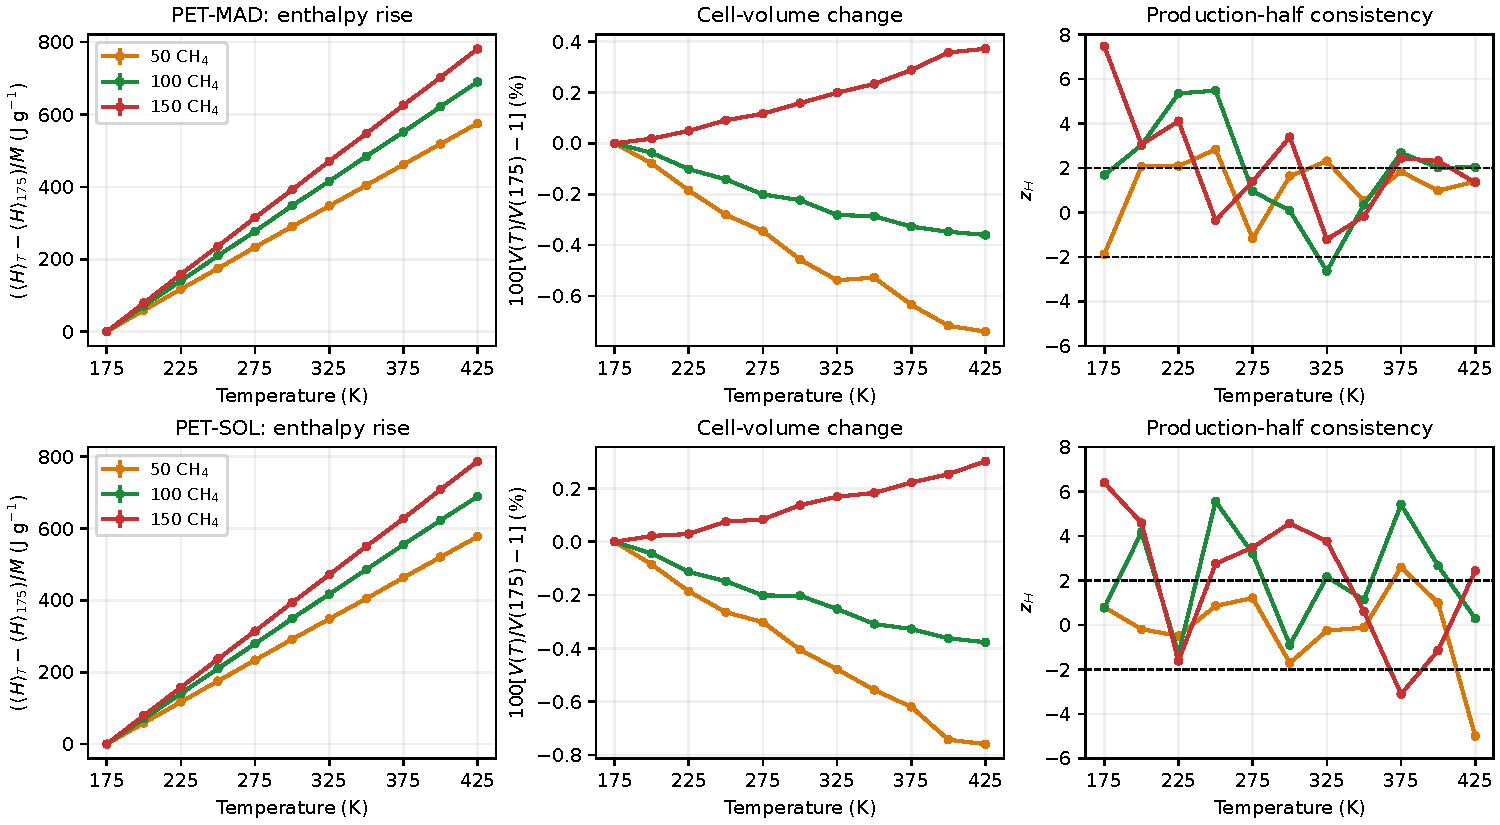
\includegraphics[width=\textwidth]{figures/results-md-overview.pdf}
  \caption{Thermodynamic diagnostics from all 66 trajectory summaries.
  Left: mass-specific enthalpy increase relative to the same model and loading
  at \SI{175}{K}; the baseline is a display offset, and the small bars show the
  pointwise enthalpy standard errors without propagating the shared baseline
  error. Middle: fractional change of mean cell volume relative to
  \SI{175}{K}. Right: the archived difference between production-half mean
  enthalpies divided by their combined standard error, $z_H$; dashed lines
  mark $\pm2$. These are diagnostics of the individual runs, not replica
  averages.}
  \label{fig:results-md-overview}
\end{figure*}

The enthalpy curves increase smoothly with temperature
(Figure~\ref{fig:results-md-overview}), giving positive classical heat
capacities. The archived enthalpy autocorrelation times are
0.095--\SI{0.101}{ps}, corresponding to approximately 1980--2115 effective
samples per trajectory instead of 8001 independent observations. Their mean
enthalpy standard errors are 0.015--\SI{0.046}{eV}. The distinction between
saved and independent samples is exactly the one in
Eq.~\eqref{eq:md-standard-error}. However, the short estimated correlation
time describes the fluctuations resolved by this estimator; it does not
exclude slower drift or unvisited states.

Indeed, 33 of the 66 runs have an absolute enthalpy split statistic greater
than two. Here the stored diagnostic is
\begin{equation}
 z_H=\frac{\overline H_{\mathrm{second}}-\overline H_{\mathrm{first}}}
 {\sqrt{\operatorname{SE}_{\mathrm{first}}^2+
              \operatorname{SE}_{\mathrm{second}}^2}}.
\end{equation}
For PET-MAD with 150 methane molecules at \SI{175}{K}, $z_H=7.47$; for
PET-SOL with 150 molecules at \SI{300}{K}, it is 4.57. A threshold crossing
is a diagnostic rather than a formal independent hypothesis test, but the
frequency and size of these discrepancies preclude a blanket claim that
\SI{100}{ps} of equilibration was sufficient. Some RMS-force time series have
correlation times as long as \SI{26.1}{ps}, with fewer than eight estimated
effective samples, illustrating that convergence is observable dependent.

\begin{figure}[t]
  \centering
  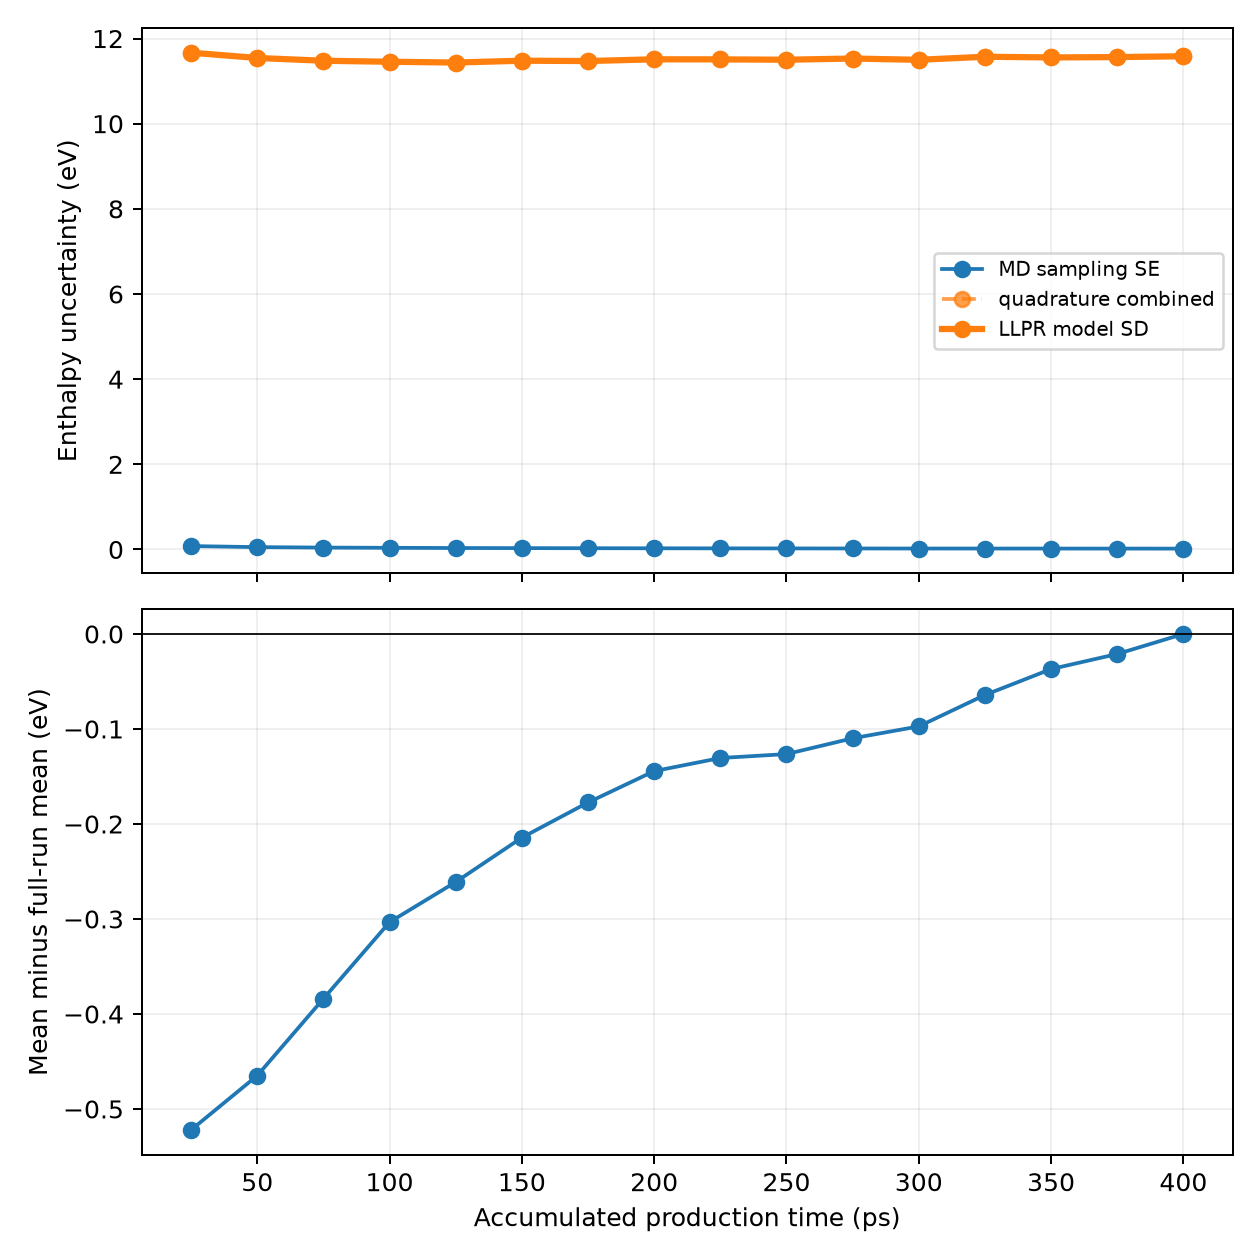
\includegraphics[width=\columnwidth]{figures/results-convergence-mad-150-175.png}
  \caption{Archived enthalpy convergence diagnostic for PET-MAD with 150
  methane molecules at \SI{175}{K}. The upper panel separates MD sampling
  error from the LLPR spread of the \emph{enthalpy}, in eV. The lower panel
  shows the accumulated mean relative to the full-production mean. Its
  endpoint is zero by construction and is not evidence of equilibration.}
  \label{fig:results-convergence}
\end{figure}

Figure~\ref{fig:results-convergence} makes the issue concrete: in the
\SI{175}{K} PET-MAD example the accumulated mean still changes appreciably as
production is extended. Its offset is about $-0.30$ eV after \SI{100}{ps} and
about $-0.15$ eV after \SI{200}{ps}, relative to the final mean. The much larger
LLPR enthalpy spread in the upper panel does not make this drift harmless:
heat capacity differentiates enthalpy, and a persistent energy offset across
temperatures can cancel whereas a temperature-dependent sampling bias does
not. Longer runs, analysis with alternative discarded intervals, and
independently initialized replicas are needed before interpreting the small
reported MD errors as complete sampling uncertainties.

\subsection{Cell response, framework motion, and methane mobility}
\label{sec:results-structure}

The volume response changes with methane loading. Between 175 and
\SI{425}{K}, PET-MAD predicts a decrease from 17146.8 to
\SI{17019.9}{\angstrom\cubed} at 50 molecules, a smaller decrease from
17170.2 to \SI{17108.4}{\angstrom\cubed} at 100 molecules, and an increase
from 17210.4 to \SI{17274.4}{\angstrom\cubed} at 150 molecules. PET-SOL
shows the same qualitative pattern. The corresponding endpoint volume
changes are about $-0.75\%$, $-0.37\%$, and $+0.3$--$0.4\%$ across the two
models. This suggests that guest loading modifies the framework's thermal
response, with contraction at lower loading and expansion at the highest
loading. The mean densities at \SI{300}{K} are approximately 0.677, 0.752,
and \SI{0.825}{g\per\centi\meter\cubed} for 50, 100, and 150 molecules,
respectively; most of this loading trend reflects the added methane mass.

This observation connects directly to Eq.~\eqref{eq:cp-cv}: thermal expansion
enters $C_P-C_V$ through $\alpha_V^2$, so negative thermal expansion does not
imply a negative $C_P-C_V$. The volume trend alone neither establishes a phase
transition nor quantifies the neglected quantum pressure--volume correction;
compressibility and consistently converged derivatives would also be needed.

\begin{figure*}[t]
  \centering
  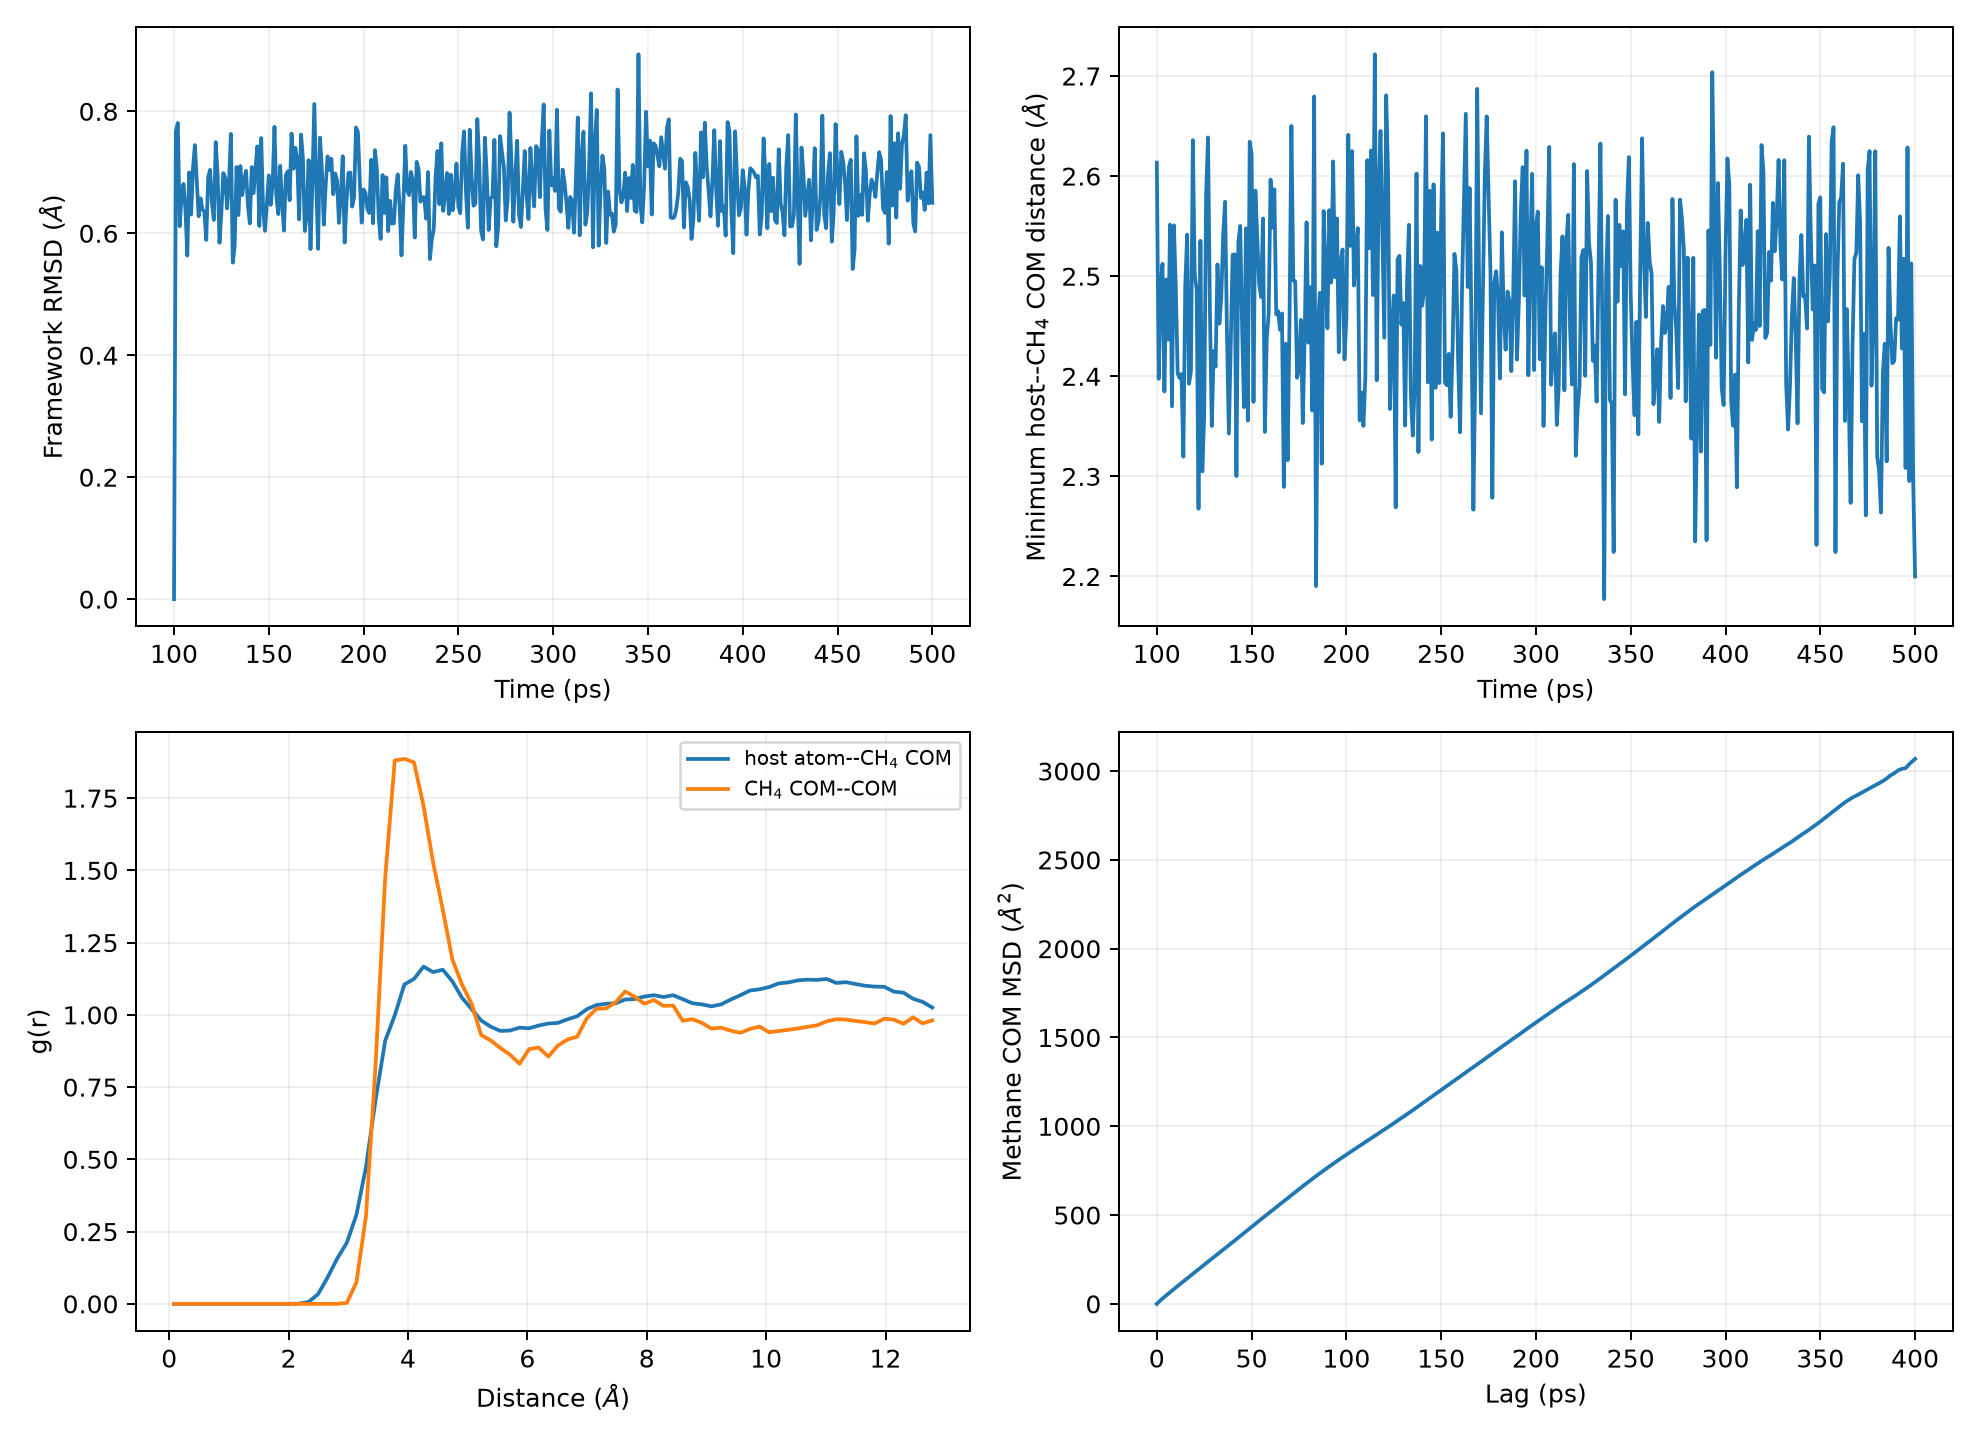
\includegraphics[width=0.85\textwidth]{figures/results-structure-sol-150-300.png}
  \caption{Structural diagnostics for PET-SOL with 150 methane molecules at
  \SI{300}{K}: framework RMSD, nearest host-atom--methane center-of-mass
  distance, radial distributions, and methane center-of-mass mean-squared
  displacement (MSD). The first analyzed frame at \SI{100}{ps} defines the
  framework reference, hence the initial zero RMSD. Long-lag MSD values use
  fewer time origins than short-lag values.}
  \label{fig:results-structure}
\end{figure*}

At \SI{300}{K}, the six mean framework RMSDs lie between 0.659 and
\SI{0.725}{\angstrom}, while the RMS changes of the tracked reference-bond
lengths are only 0.055--\SI{0.059}{\angstrom}. In the PET-SOL 150-molecule
example (Figure~\ref{fig:results-structure}), the framework fluctuates around
a bounded RMSD instead of displaying continued displacement growth. This
combination is consistent with collective framework motion without a gross
collapse of the tracked structure over the analyzed interval. It is not a
complete test of chemical integrity: the diagnostics track a reference
neighbor set and do not establish the absence of every possible bond change.

Methane remains mobile. At \SI{300}{K}, the \SI{400}{ps} MSD is approximately
$8.9$--$9.2\times10^3\,\text{\AA}^2$ at 50 molecules,
$5.1$--$5.6\times10^3\,\text{\AA}^2$ at 100 molecules, and
$3.1$--$3.4\times10^3\,\text{\AA}^2$ at 150 molecules.
The lower displacement at higher loading is consistent with hindered guest
motion as the pores become more crowded. The methane center-of-mass radial
distributions have their first prominent peak near \SI{4}{\angstrom},
showing local guest organization alongside translational mobility.
These diagnostics support the need for the anharmonic MD term in
Eq.~\eqref{eq:hybrid-cp}: diffusion and changing adsorption environments
cannot be generated by a harmonic expansion about one geometry. No diffusion
coefficient is inferred here from the endpoint MSD; a defensible fit would
require a verified diffusive regime, control of cell-motion effects,
adequate time-origin statistics, and replica uncertainty.

\subsection{Classical, harmonic, and hybrid heat capacities}
\label{sec:results-cp}

Figures~\ref{fig:results-cp-mad} and \ref{fig:results-cp-sol} show the supplied
loading-comparison curves with the refreshed CEA uncertainty bands.
Table~\ref{tab:results-cp} resolves the contributions at \SI{300}{K}.
For PET-MAD, increasing loading from 50 to 150 molecules raises the classical
term from 2.281 to \SI{3.122}{J\per g\per K}; for PET-SOL the corresponding
range is 2.289--\SI{3.134}{J\per g\per K}. The quantum-minus-classical
harmonic correction is negative, ranging from approximately $-1.35$ to
$-1.97\,\mathrm{J\,g^{-1}\,K^{-1}}$ across the six systems. It removes
roughly 59--63\% of the classical heat capacity at this temperature.

The large reduction is the expected signature of classical equipartition
populating high-frequency framework and methane vibrations too strongly.
It follows from the quantum oscillator contribution in
Eq.~\eqref{eq:quantum-harmonic-cv}: a thermally inaccessible mode contributes
less than the classical $k_{\mathrm B}$. The increasingly negative correction
with loading also demonstrates why the empty-framework spectrum cannot
replace the loaded-system Hessian. Both the additional methane internal
modes and mixed host--guest modes enter the correction.

\begin{table*}[t]
  \centering
  \small
  \caption{Heat capacities and uncertainty estimates at \SI{300}{K}, all in
  \si{J\per g\per K} and normalized by the total mass of each loaded cell.
  $c_{\mathrm{cl}}$ is the central enthalpy derivative, $\Delta c_{\mathrm{har}}$
  the retained-mode harmonic correction, and $c_{\mathrm{hyb}}$ their sum.
  $u_{\mathrm{CEA}}$ and $u_{\mathrm G}$ use different paired model spreads
  around the \emph{same} central value and MD standard error
  $\sigma_{\mathrm{MD}}$. The final column is the separate variance-based
  central hybrid estimate. None of these uncertainties includes the bias
  from discarded imaginary modes or an estimated spread across minima.}
  \label{tab:results-cp}
  \begin{tabular}{@{}lrrrrrrrr@{}}
    \toprule
    Model & $N_{\chfour}$ & $c_{\mathrm{cl}}$ & $\Delta c_{\mathrm{har}}$
    & $c_{\mathrm{hyb}}$ & $\sigma_{\mathrm{MD}}$ & $u_{\mathrm{CEA}}$
    & $u_{\mathrm G}$ & $c_{\mathrm{hyb}}^{\mathrm{var}}$ \\
    \midrule
PET-MAD & 50 & 2.281 & -1.351 & 0.929 & 0.010 & 0.068 & 0.127 & 0.926 \\
PET-MAD & 100 & 2.762 & -1.682 & 1.080 & 0.010 & 0.123 & 0.169 & 1.044 \\
PET-MAD & 150 & 3.122 & -1.957 & 1.165 & 0.010 & 0.113 & 0.214 & 1.202 \\
PET-SOL & 50 & 2.289 & -1.363 & 0.926 & 0.010 & 0.087 & 0.150 & 0.940 \\
PET-SOL & 100 & 2.762 & -1.693 & 1.069 & 0.010 & 0.153 & 0.225 & 1.024 \\
PET-SOL & 150 & 3.134 & -1.969 & 1.166 & 0.010 & 0.103 & 0.306 & 1.230 \\
    \bottomrule
  \end{tabular}
\end{table*}

\begin{figure*}[t]
  \centering
  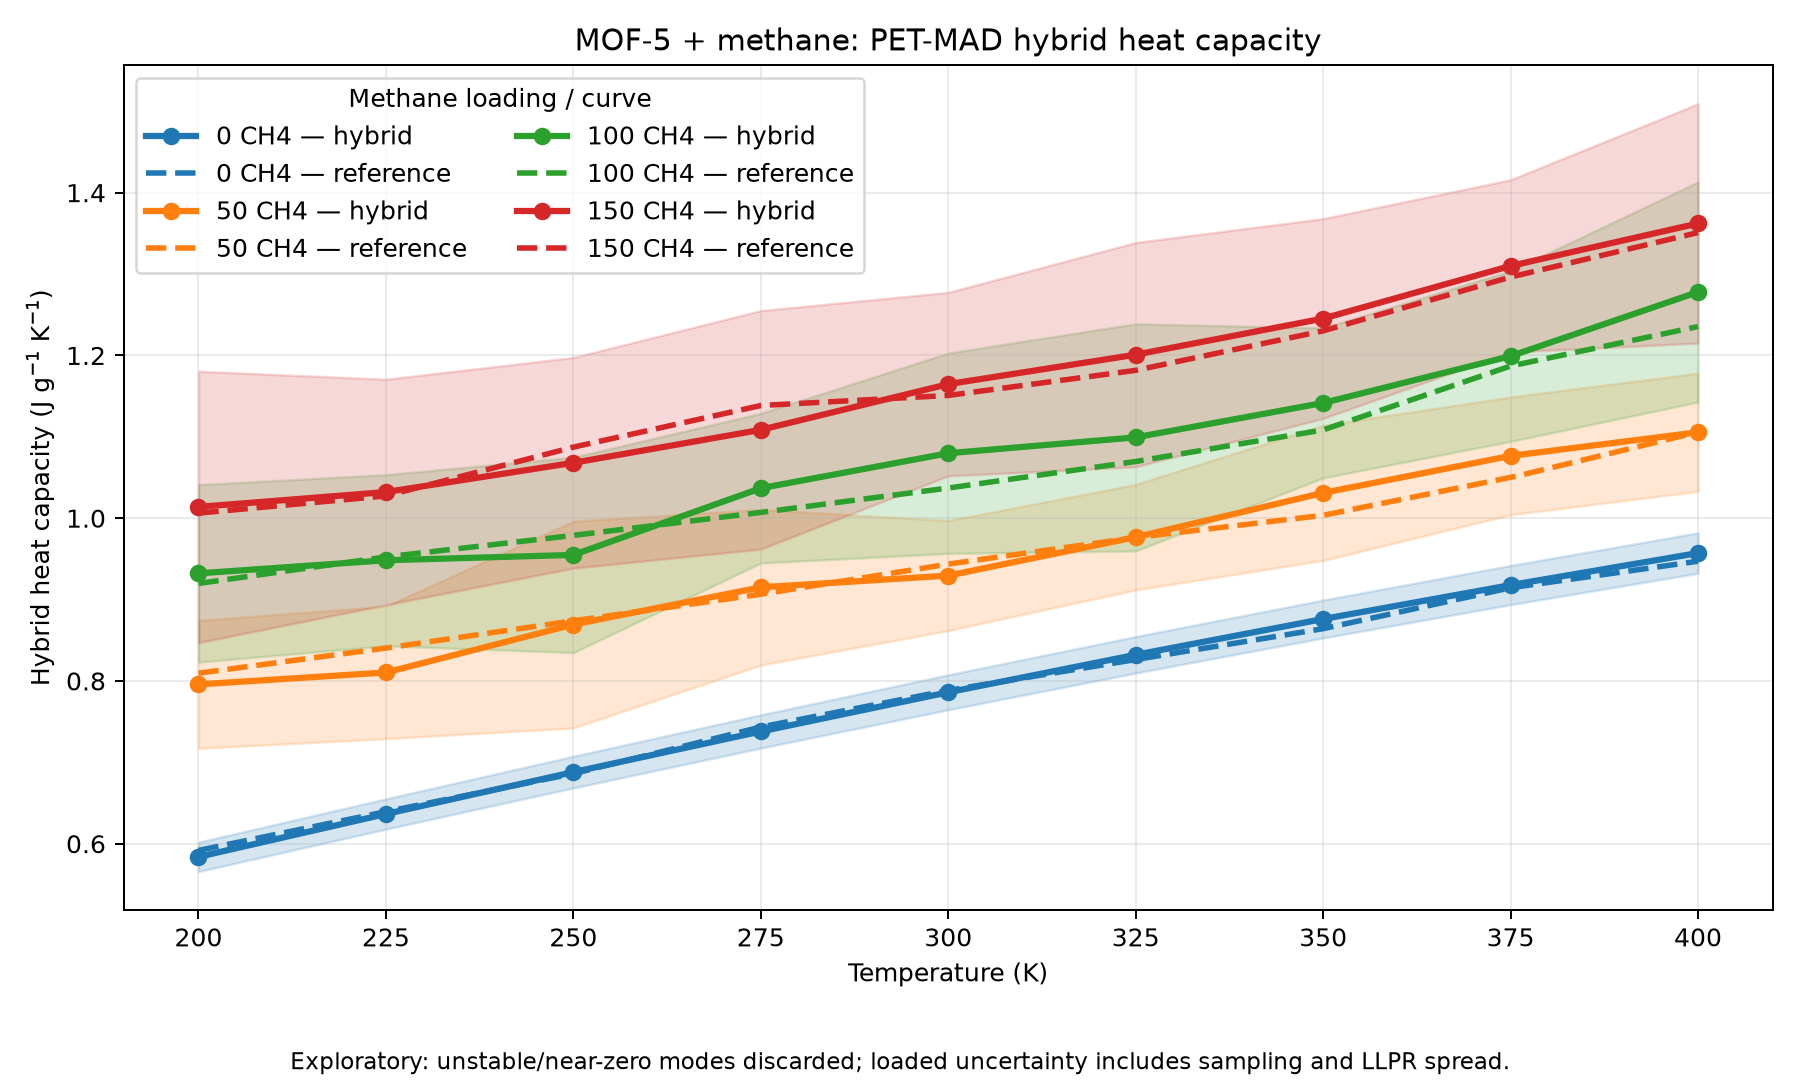
\includegraphics[width=0.90\textwidth]{figures/results-pet-mad-cea.png}
  \caption{Supplied PET-MAD loading comparison. Loaded solid curves are
  central classical enthalpy derivatives plus retained-mode harmonic quantum
  corrections. Their shading is $\pm u_{\mathrm{CEA}}$, combining MD sampling
  error with correlated classical--harmonic LLPR spread. Despite the common
  ``hybrid'' legend, the zero-loading curve is a quantum-harmonic $c_V$
  calculation only, with a harmonic LLPR band; no empty-system MD term was
  computed. Dashed curves are the supplied reference CSVs, whose provenance
  is discussed in the text.}
  \label{fig:results-cp-mad}
\end{figure*}

\begin{figure*}[t]
  \centering
  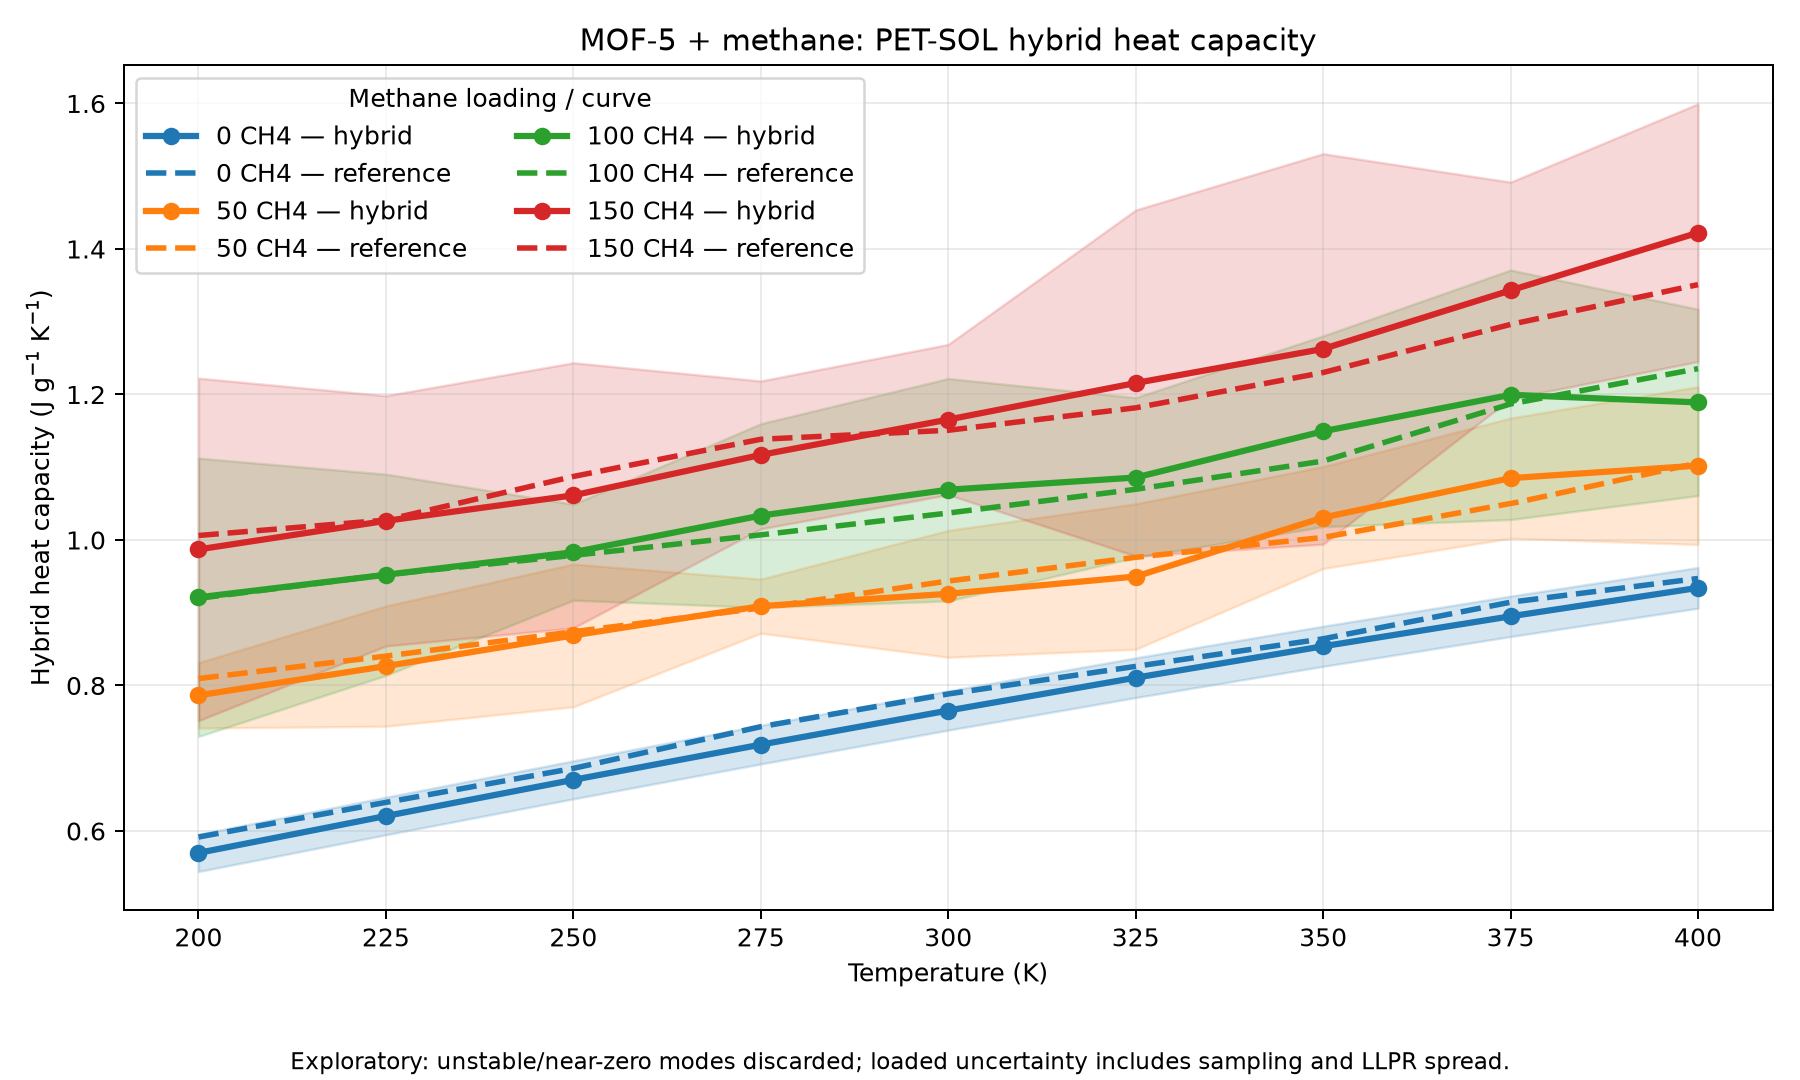
\includegraphics[width=0.90\textwidth]{figures/results-pet-sol-cea.png}
  \caption{Supplied PET-SOL loading comparison, with the same definitions
  and exploratory mode treatment as Figure~\ref{fig:results-cp-mad}.
  The slight decrease of the 100-molecule central curve at the upper end of
  the grid is smaller than its uncertainty band and is not evidence of a
  resolved thermodynamic anomaly. Shading denotes standard uncertainty,
  not a calibrated confidence interval.}
  \label{fig:results-cp-sol}
\end{figure*}

The net room-temperature hybrid values are approximately 0.93, 1.07--1.08,
and \SI{1.16}{J\per g\per K} for 50, 100, and 150 methane molecules.
The PET-MAD and PET-SOL central values differ by only 0.003, 0.011, and
\SI{0.001}{J\per g\per K}, respectively. These differences are much smaller
than the propagated model bands, so the calculations do not distinguish the
two potentials' predictive accuracy. Agreement can also reflect shared
modeling assumptions and cannot be used as independent validation of the
harmonic approximation.

Across 200--\SI{400}{K}, the PET-MAD loaded curves rise from
0.796, 0.932, and 1.014 to 1.106, 1.278, and
\SI{1.362}{J\per g\per K}. PET-SOL gives corresponding endpoints
0.787, 0.921, and 0.987, and 1.102, 1.189, and
\SI{1.422}{J\per g\per K}. Increasing thermal occupation makes the harmonic
correction less negative, contributing to the upward temperature trend even
where the classical term changes little. For example, the PET-MAD
50-molecule classical term changes from 2.347 to
\SI{2.269}{J\per g\per K}, while its correction changes from $-1.551$ to
$-1.164\,\mathrm{J\,g^{-1}\,K^{-1}}$. The positive slope of the final curve
therefore should not be attributed solely to increasing classical
anharmonicity.

The broad ordering with loading is common to both models, but adjacent
loading bands overlap substantially. Quantitative significance of a
loading difference would require propagating the \emph{difference} with
persistent member identities, not merely inspecting overlap of marginal
bands. The reported range starts at \SI{200}{K}; it does not bracket a
low-temperature minimum and cannot verify the minimum discussed in
Section~\ref{sec:reference-conclusions}. Small local bends, such as the
PET-SOL 100-molecule turnover near \SI{400}{K}, remain sensitive to finite
sampling and temperature differentiation.

The empty-system values at \SI{300}{K} are
$0.786\pm0.021$ for PET-MAD and
$0.766\pm0.027\,\mathrm{J\,g^{-1}\,K^{-1}}$ for PET-SOL. These are
quantum-harmonic $c_V$ values with LLPR model standard deviations, separately
normalized by the framework mass. They are not a full hybrid $c_P$ and do
not measure the incremental heat capacity of adsorbing one methane molecule.
The dashed reference curves were digitized from Kapil \emph{et al.}\
\cite{kapil2019}, as confirmed for the supplied reference CSVs. At
\SI{300}{K} those files give approximately 0.788, 0.944, 1.037, and
\SI{1.151}{J\per g\per K} for 0, 50, 100, and 150 methane molecules.
The broad loading and temperature trends agree with the present curves, and
the loaded room-temperature differences are at most about
\SI{0.043}{J\per g\per K}. This is a contextual comparison, not validation:
the digitized points contain no uncertainty estimates, the underlying force
fields and preparation protocols differ (Section~\ref{sec:reference-comparison}),
and the present spectra and sampling have unresolved limitations. The
approximate empty-framework scale quoted earlier is less precise than these
digitized values and should not be treated as a separate numerical target.

\subsection{Hessian stability and interpretation of the quantum correction}
\label{sec:results-hessians}

\begin{table*}[t]
  \centering
  \small
  \caption{Archived central loaded-Hessian diagnostics. All calculations use
  PET-JAX, float64, three graph hops, and the force-constant row-sum acoustic
  treatment. ``Converged'' reproduces the relaxation archive's flag for its
  requested tolerance. Imaginary modes have signed frequencies below
  $-1\,\mathrm{cm^{-1}}$; near-zero modes satisfy
  $|\widetilde\nu|\leq1\,\mathrm{cm^{-1}}$. Retained modes have positive
  frequencies above the threshold. Signed negative values represent
  unstable curvature, not physical negative-frequency oscillators.}
  \label{tab:results-hessians}
  \begin{tabular}{@{}lrr rrrr r@{}}
    \toprule
    Model & $N_{\chfour}$ & Converged & $F_{\max}$ & Imaginary & Near zero
      & Retained & $\widetilde\nu_{\min}$ \\
    & & & (eV/\AA) & & & & ($\mathrm{cm^{-1}}$) \\
    \midrule
PET-MAD & 50 & no & 0.0170 & 17 & 5 & 2000 & -53.5 \\
PET-MAD & 100 & yes & 0.0097 & 114 & 3 & 2655 & -92.4 \\
PET-MAD & 150 & no & 0.0095 & 28 & 3 & 3491 & -66.8 \\
PET-SOL & 50 & no & 0.0054 & 32 & 3 & 1987 & -107.7 \\
PET-SOL & 100 & yes & 0.0100 & 95 & 3 & 2674 & -138.4 \\
PET-SOL & 150 & no & 0.0049 & 35 & 3 & 3484 & -86.5 \\
    \bottomrule
  \end{tabular}
\end{table*}

Table~\ref{tab:results-hessians} prevents interpreting a small residual force
as proof of a valid harmonic minimum. The two 100-molecule structures meet
their archived force criteria, yet have 114 and 95 imaginary modes for
PET-MAD and PET-SOL. The most negative signed frequencies are
$-92.4$ and $-138.4\,\mathrm{cm^{-1}}$, far beyond the
$1\,\mathrm{cm^{-1}}$ exclusion threshold. The other loadings retain
17--35 imaginary modes and are flagged unconverged. The force tolerances
are run dependent: a smaller final force in one run does not override that
run's failed convergence flag. PET-MAD at 50 molecules also has five
near-zero modes, exceeding the three translational modes expected for a
stable periodic structure.

Section~\ref{sec:normal-modes} relates squared frequencies to eigenvalues of
the mass-weighted Hessian. Negative eigenvalues signal directions in which
the quadratic energy decreases. Discarding them makes the oscillator sum
numerically evaluable, but does not make the reference geometry a stable
minimum. The cause cannot be assigned from these archives alone: insufficient
relaxation, unstable stationary structures, sparse-Hessian truncation, or
other curvature errors must be distinguished by convergence checks. The empty
spectra also contain four and five imaginary modes, with minima of
$-5.5$ and $-6.6\,\mathrm{cm^{-1}}$, so their stability is not established
either, although their negative curvatures are much smaller.

Using the same retained-mode mask in the quantum and classical terms avoids
subtracting a different number of modes, as required by
Section~\ref{sec:hybrid-method}. It does not quantify the missing anharmonic
physics of an unstable direction. Nor does reusing one \SI{400}{K} spectrum
establish that its curvature represents every temperature. With one quenched
geometry per model and loading, the stored zero harmonic sampling error means
that minimum-to-minimum variation was not estimated. The LLPR Hessian spread
varies the energy readout at the fixed central geometry; it does not replace
that missing structural sampling or include member-specific relaxation.

\subsection{What determines the uncertainty bands?}
\label{sec:results-uncertainty}

Figures~\ref{fig:results-error-cea} and \ref{fig:results-error-gaussian}
separate the uncertainty contributions. The blue MD sampling error of the
enthalpy derivative is small, approximately
\SI{0.010}{J\per g\per K} at \SI{300}{K}. The green harmonic LLPR spread is
larger and generally increases with loading. The orange classical spread
is obtained either by differentiating the CEA member enthalpies
[Eq.~\eqref{eq:llpr-cp-spread}] or by the Gaussian NPT approximation of
Section~\ref{sec:gaussian-propagation}. The red total uses the standard
deviation of the \emph{paired sum} of classical and harmonic member
contributions, then combines this with MD sampling error. Thus it need not
exceed every individual model contribution.

\begin{figure*}[t]
  \centering
  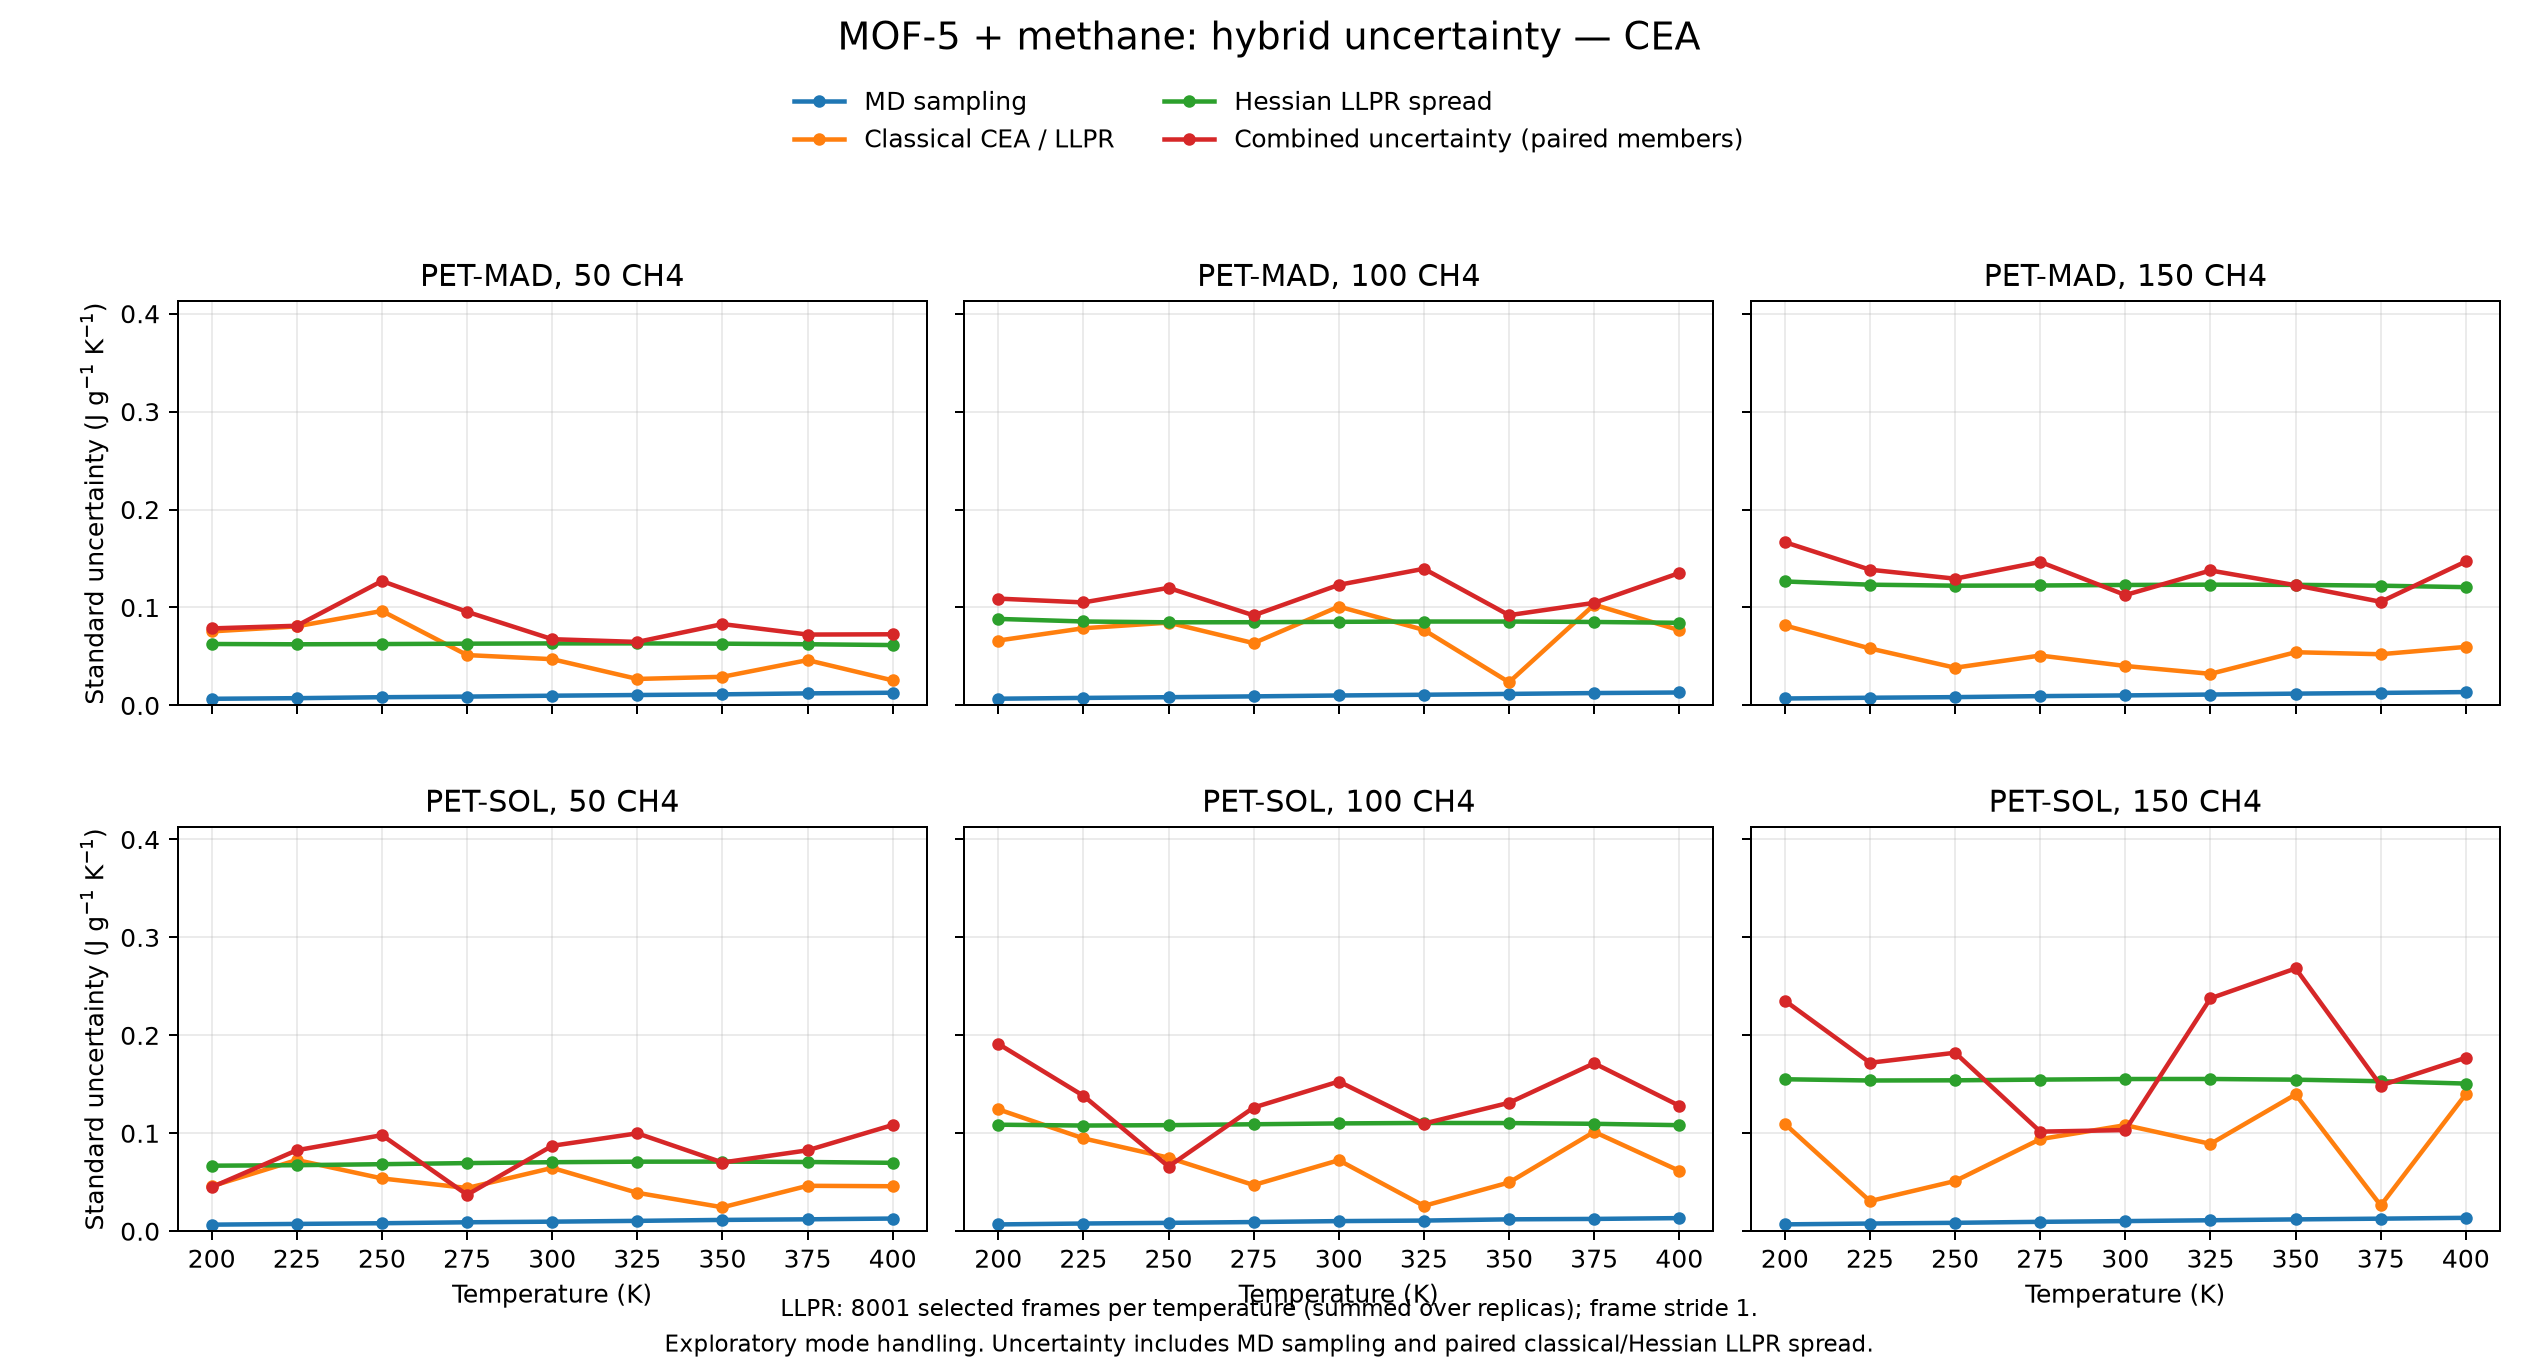
\includegraphics[width=\textwidth]{figures/results-uncertainty-cea.png}
  \caption{Supplied uncertainty decomposition using refreshed CEA member
  curves. Every panel uses all 8001 saved production frames at each
  temperature and 64 LLPR members. The harmonic curve is model spread at
  one fixed geometry, not an uncertainty across minima. The total preserves
  classical--harmonic covariance and excludes an unestimated harmonic
  sampling term. All plotted quantities are standard errors or model standard
  deviations in \si{J\per g\per K}, not variance fractions.}
  \label{fig:results-error-cea}
\end{figure*}

For example, PET-SOL at 150 molecules and \SI{300}{K} has classical and
harmonic CEA-based model standard deviations of 0.108 and
\SI{0.155}{J\per g\per K}. Their paired hybrid spread is only
\SI{0.103}{J\per g\per K}, corresponding to an inferred member correlation
of approximately $-0.75$. Conversely, PET-SOL at 100 molecules has positive
correlation (approximately $+0.37$), increasing the paired spread to
\SI{0.153}{J\per g\per K}. Summing the separate model variances as if
independent would miss both effects. Model spread is not divided by
$\sqrt{64}$, because it describes variations of predicted properties across
the ensemble rather than the uncertainty of repeated measurements of one
fixed mean.

\begin{figure*}[t]
  \centering
  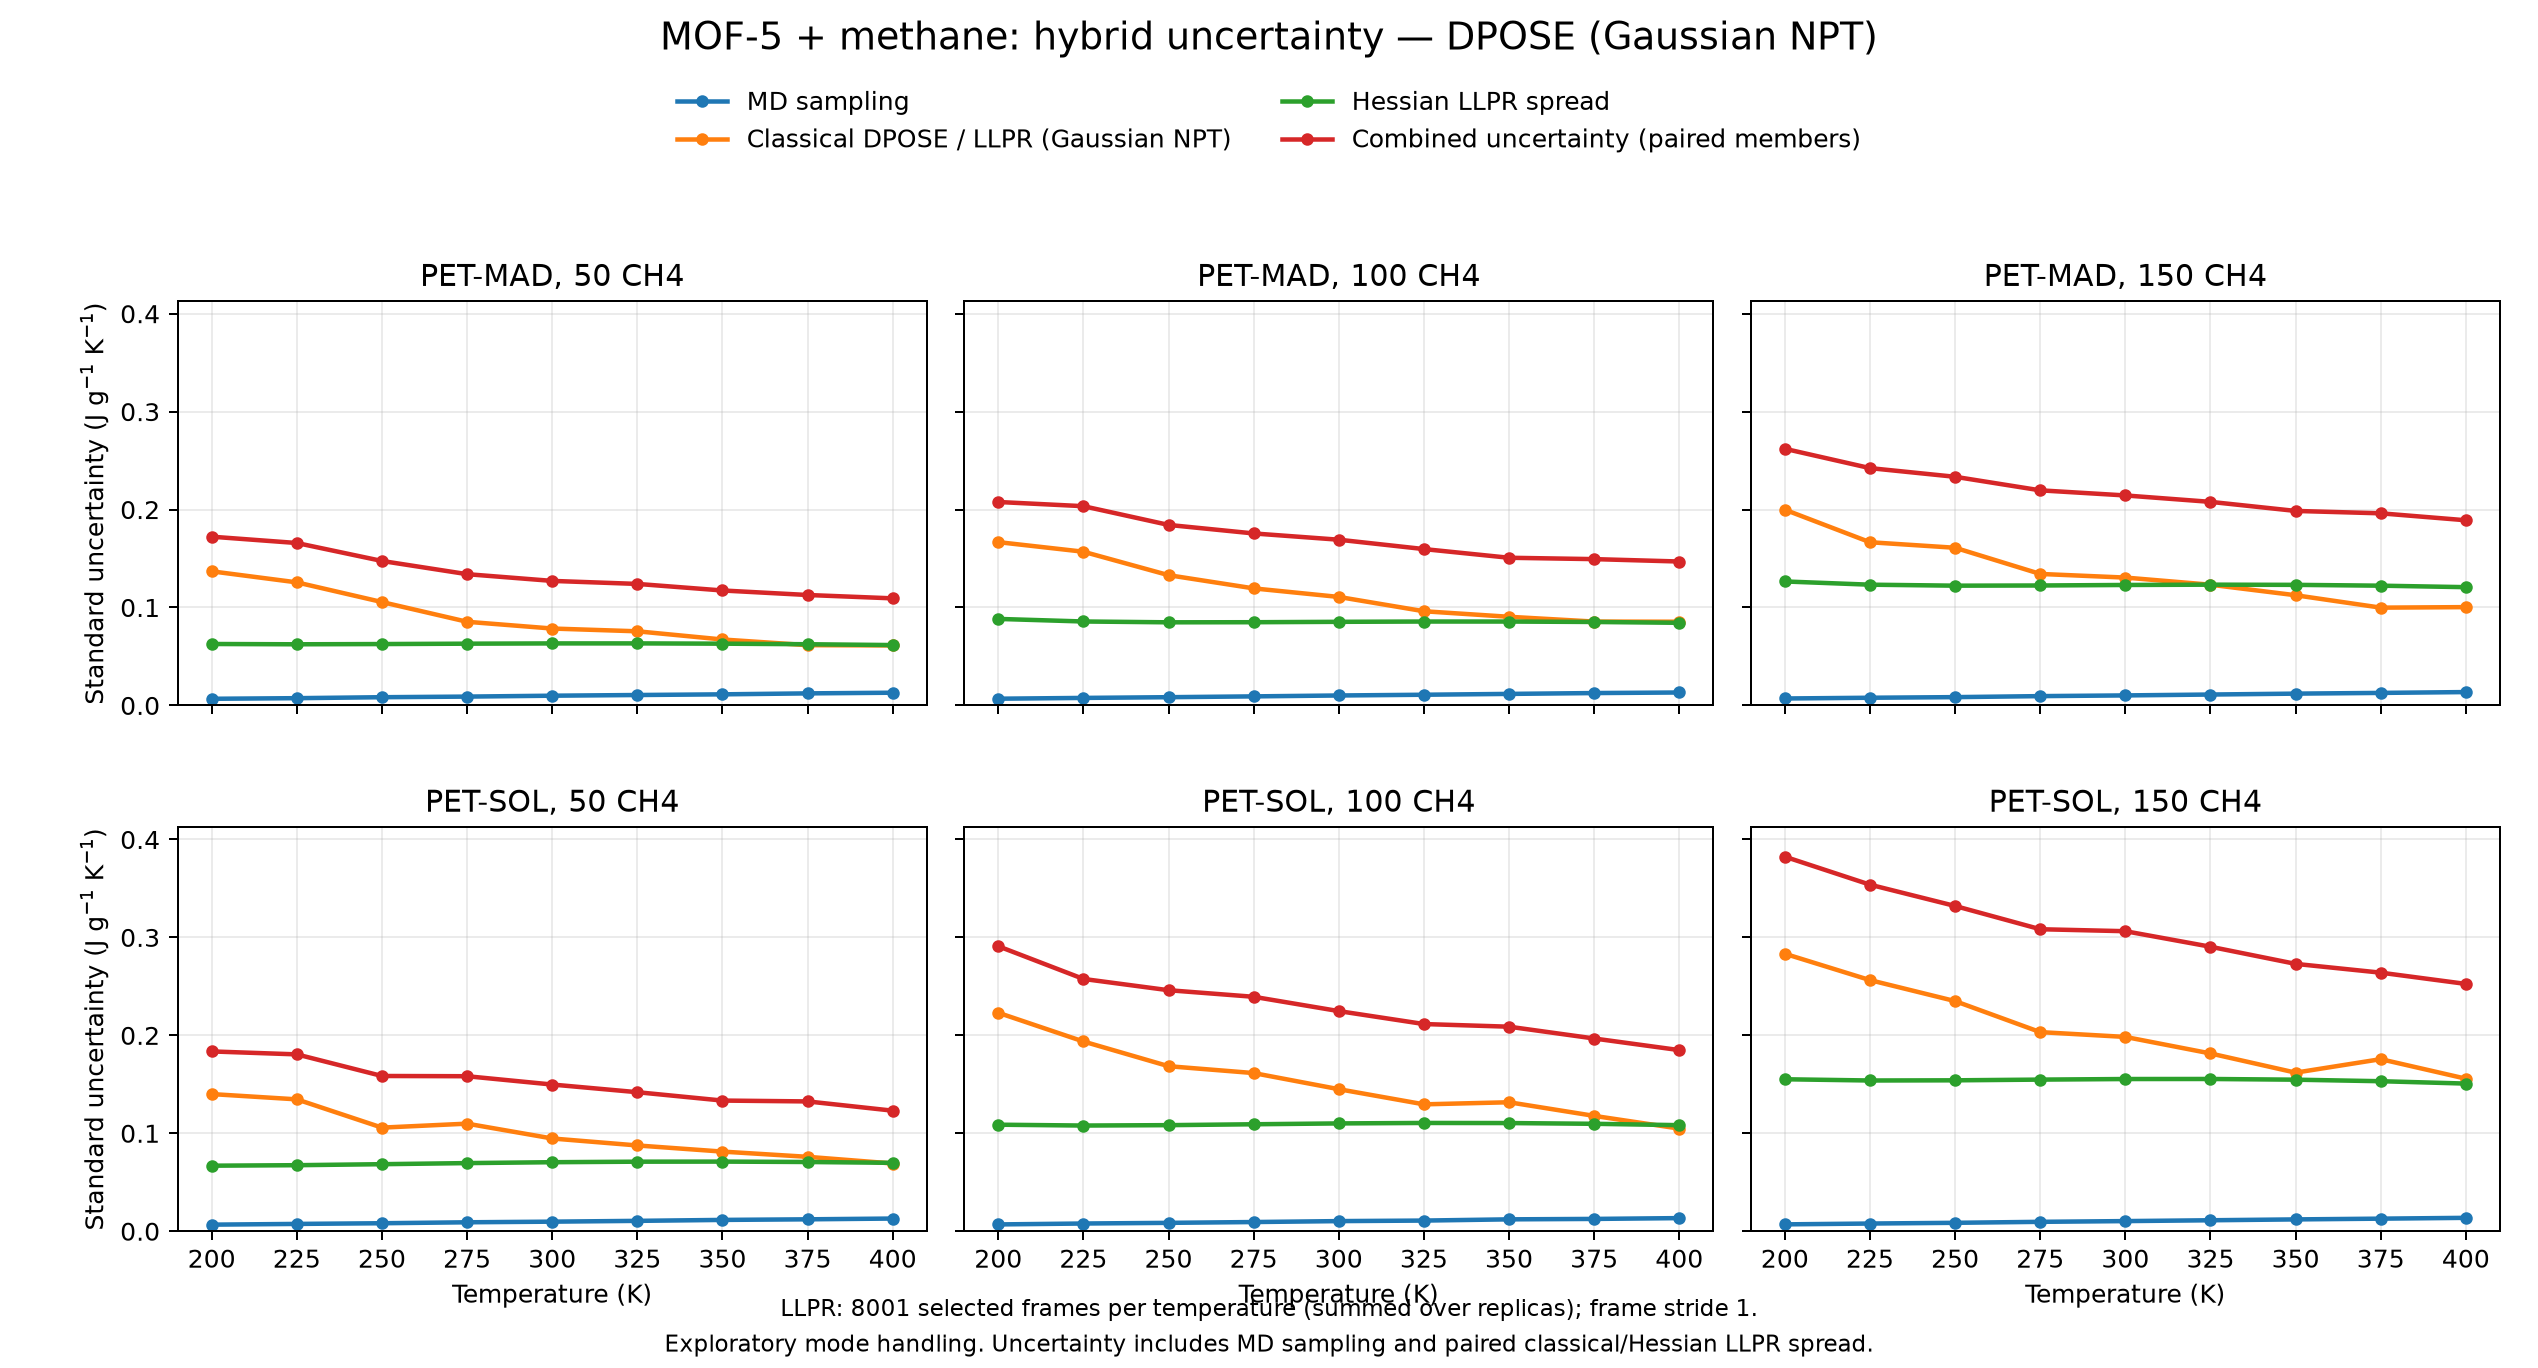
\includegraphics[width=\textwidth]{figures/results-uncertainty-gaussian.png}
  \caption{Supplied Gaussian NPT/DPOSE uncertainty decomposition. Central
  hybrid curves, MD sampling errors, harmonic member corrections, and frame
  coverage are identical to the CEA comparison; only the classical member
  spread and its covariance with the harmonic correction change. The smoother
  orange curves result from a different estimator and do not establish more
  accurate uncertainty calibration.}
  \label{fig:results-error-gaussian}
\end{figure*}

In the refreshed \SI{300}{K} comparison, Gaussian propagation gives larger
combined bands in every model--loading case: for PET-MAD they are
0.127, 0.169, and \SI{0.214}{J\per g\per K}, compared with CEA values
0.068, 0.123, and \SI{0.113}{J\per g\per K}. For PET-SOL the corresponding
Gaussian values are 0.150, 0.225, and \SI{0.306}{J\per g\per K}, compared
with 0.087, 0.153, and \SI{0.103}{J\per g\per K} for CEA. Gaussian
classical--harmonic correlations at this temperature are positive in all six
cases, approximately 0.43--0.63. The method dependence of both the classical
spread and its covariance is therefore material to the reported uncertainty.

These differences should not be interpreted as proof that the narrower or
smoother band is correct. Across all runs and members, the recorded
$\operatorname{var}(\beta\Delta U_i)$ ranges from approximately 2.4 to
$1.42\times10^3$, rather than being much smaller than one as required for
a controlled first-order CEA. Direct-reweighting effective sample counts
approach one for some members. Consequently, exact reweighting is not a
reliable independent validation of CEA for those members, and Gaussian
tail behavior also needs checking. The bands are conditional diagnostics
of these propagation approximations; their statistical coverage against
reference electronic-structure data has not been demonstrated here.

The separate \texttt{variance-hybrid} results change the \emph{central}
classical estimator as well as its sampling error. Their \SI{300}{K} hybrid
values are listed in the final column of Table~\ref{tab:results-cp}; they
differ from the derivative-based values by approximately $-0.045$ to
$+0.064\,\mathrm{J\,g^{-1}\,K^{-1}}$. Their MD sampling errors are
0.022--\SI{0.030}{J\per g\per K}, larger than those of the enthalpy
derivative, and are estimated from the autocorrelation of squared
configurational-enthalpy fluctuations. For the central potential this is a
fluctuation estimator of the same classical NPT response
(Section~\ref{sec:md-response}); Gaussian closure is needed to infer the
member-ensemble variances from the central trajectory. Agreement in overall
scale is a useful check, but the two estimates share trajectories and
harmonic corrections and therefore are not independent measurements.

Taken together, the outputs support a positive loading dependence, a large
quantum reduction of the classical heat capacity, and substantial guest
mobility. They also identify the immediate requirements for a quantitative
prediction: resolve the unstable Hessian spectra, establish stationarity
with longer independent trajectories, sample more quenched structures, and
validate propagation under representative LLPR members. Reducing the already
small reported MD standard error alone will not resolve these limitations.

\clearpage

\section{Recommended production and analysis protocol}

\subsection{Empty MOF-5 reference}

The equilibrated empty-framework structure is used directly; an empty-MOF MD
campaign would add cost without supplying the anharmonic loaded-system term
needed by Eq.~\eqref{eq:hybrid-cp}.

\begin{enumerate}
  \item Relax the atomic coordinates with the same PET-MAD checkpoint used for
        the Hessian. Report maximum residual force and do not relax the cell
        unless a stress-capable, validated model is adopted.
  \item Check stability using signed eigenvalues and inspect low-frequency
        modes. A large number of unstable modes invalidates the harmonic
        interpretation.
  \item Converge float32 against float64, graph hops, HVP chunking, acoustic
        sum-rule treatment, and frequency threshold.
  \item Converge the conventional-cell result with respect to supercell size or
        phonon wave-vector sampling. A single periodic cell Hessian samples
        only the corresponding finite set of modes.
  \item Retain the resulting curve as a separately normalized reference and
        compare its room-temperature value with the approximately
        \SI{0.7}{J\per g\per K} published reference scale as a contextual
        check, not a fitting target; PET-MAD replaces QuickFF and its model
        error remains to be quantified.
\end{enumerate}

\subsection{Loaded MOF-5 production and Hessians}

For the 100-methane system, the production sequence is:

\begin{enumerate}
  \item Prepare independent methane placements and velocity seeds for each
        replica on the enthalpy temperature grid.
  \item Run flexible-cell classical NPT only for the loaded system. Determine
        equilibration from enthalpy, cell, framework, and methane-mobility
        diagnostics rather than assuming the template duration is sufficient.
  \item Average enthalpy over the stationary part of each replica, combine
        replica uncertainties, and differentiate the temperature dependence.
  \item Select representative independent loaded configurations, quench each
        one to a fixed-cell minimum with the same MLIP, and reject unconverged
        or unstable minima.
  \item Compute one AD Hessian per accepted minimum. Converge precision, graph
        hops, HVP chunking, acoustic treatment, frequency threshold, and cell
        size on the quantum-minus-classical correction.
  \item Average the loaded corrections, combine them with the classical
        enthalpy derivative using Eq.~\eqref{eq:hybrid-cp}, and report MD and
        minimum-to-minimum uncertainties separately as well as jointly.
\end{enumerate}

This calculation applies the hybrid method, rather than attempting an exact
reproduction of the reference study. Its success is assessed by internal
numerical convergence and by validation of the PET potential for the relevant
structures; quantitative accuracy below approximately \SI{200}{K} remains to
be established for the selected MLIP and loading.

\subsection{Equilibration and convergence criteria}

Production decisions should be based on observables, not a fixed waiting time
alone. At minimum, inspect:

\begin{itemize}
  \item running and block averages of temperature, potential energy, and total
        energy;
  \item maximum and distribution of force magnitudes;
  \item framework bond integrity, pore geometry, and cell consistency;
  \item methane center-of-mass distributions, host--guest distances, and
        mean-squared displacements;
  \item sensitivity to timestep and thermostat friction;
  \item agreement among independent seeds;
  \item convergence of the enthalpy derivative with replica count, sampling
        length, and temperature spacing; and
  \item convergence of the harmonic correction with independent minima,
        precision, sparsity depth, cell size, and mode treatment.
\end{itemize}

The timestep should first be validated in short NVE tests by checking energy
drift. Thermostat convergence should then be tested separately, because a
thermostat can conceal an integration error while maintaining the desired
kinetic temperature.

\section{Implementation, outputs, and reproducibility}

The production campaign is prepared by
\texttt{python -m mof\_heat\_capacity.protocols.loaded} and submitted by
\texttt{simulation/submit\_loaded\_md.sh}. These commands create independent
loaded structures and LAMMPS/metatomic NPT runs while deliberately rejecting a
zero-methane MD campaign. Trajectory diagnostics are submitted with
\texttt{properties/submit\_analysis.sh}.

The command \texttt{properties/submit\_heat\_capacity.sh} takes final structures
from selected loaded replicas, relaxes them with
\texttt{mof\_heat\_capacity.structures.relax}, and passes the optimized
structures to \texttt{mof\_heat\_capacity.analysis.harmonic}. The same command
relaxes and evaluates the supplied empty reference directly. Harmonic archives
store the run and model identity, optimized structure, temperature grid,
frequency array, gravimetric \cv{} curve, precision, graph hops, HVP chunk
size, and rematerialization choice. Finally,
\texttt{properties/submit\_hybrid\_analysis.sh} differentiates the loaded NPT
enthalpies and writes the classical term, harmonic correction, combined curve,
uncertainties, and provenance as NPZ, CSV, and JSON files.

The uncertainty calculations and their stored locations are summarized in
Table~\ref{tab:uncertainty-outputs}.

\begin{table*}[t]
\centering
\small
\caption{Uncertainty components, their calculation locations, and their
stored outputs.}
\label{tab:uncertainty-outputs}
\begin{tabular}{@{}p{3.3cm}p{5.0cm}p{5.4cm}@{}}
\toprule
Quantity & Where it is calculated & Stored result \\
\midrule
LLPR energy standard deviation & metatrain LLPR covariance and calibration &
\texttt{energy\_uncertainty}; copied as
\texttt{analytical\_energy\_uncertainty\_eV} in the per-run archive \\
CEA member enthalpies and overlap diagnostics &
\texttt{analysis/uncertainty.py}, function
\texttt{committee\_enthalpy\_estimates} & per-run
\texttt{model\_uncertainty.npz} \\
Classical LLPR $C_P$ standard deviation &
\texttt{analysis/results.py}, after member-wise replica averaging and
temperature differentiation &
\texttt{model\_uncertainty\_heat\_capacity.npz} and \texttt{.csv} \\
MD sampling standard error &
\texttt{analysis/statistics.py}, then replica combination and derivative
resampling in \texttt{analysis/hybrid.py} &
\texttt{classical\_anharmonic\_cp\_standard\_error} \\
Harmonic sampling standard error &
\texttt{analysis/hybrid.py}, across independent optimized minima &
\texttt{harmonic\_quantum\_correction\_standard\_error} \\
Hessian LLPR standard deviation &
\texttt{analysis/harmonic.py}, after differentiating persistent LLPR readouts
at the central minimum &
\texttt{harmonic\_quantum\_correction\_model\_standard\_deviation} \\
Combined standard uncertainty & quadrature in
\texttt{analysis/hybrid.py} &
\texttt{approximate\_cp\_combined\_standard\_uncertainty} \\
\bottomrule
\end{tabular}
\end{table*}

The scalar analytical LLPR energy uncertainty is archived but is not used
directly as the heat-capacity error. That error is calculated only after CEA
has produced a complete enthalpy curve for every persistent ensemble member.
The PET-JAX Hessian calculation uses the same persistent LLPR readouts and the
hybrid model spread preserves their correlation with the classical CEA term.
The Hessians are evaluated at the central-model minima; member-resolved
geometry optimization is not included.

Cluster calculations use one node, one task, and one GPU because neither the MD
nor Hessian code is MPI or multi-GPU parallel. Independent temperature,
replica, or optimized-minimum jobs are the available level of parallelism.
Slurm job identifiers and resource use should be retained; elapsed time and peak
memory can be recovered with, for example,
\begin{verbatim}
sacct -j JOB_ID \
  --format=JobID,State,Elapsed,\
MaxRSS,AllocTRES
\end{verbatim}
Wall time and memory requests should be based on representative jobs.
Separate output directories and
prefixes are required for every loading, temperature, seed, and replica.

A reproducible result should record:

\begin{itemize}
  \item source structure, cell, atom count, chemical composition, loading, and
        methane-insertion seed and rejection criteria;
  \item PET-MAD checkpoint hash, metatomic export, PET-JAX conversion, software
        environment, device, and numerical precision;
  \item LLPR covariance and calibration dataset hashes, energy-label
        definition, regularizer, calibration method, random seed, member
        count, exported ensemble hash, frame stride, and CEA diagnostics;
  \item ensemble, target temperature, timestep, thermostat and friction,
        number of steps, output stride, velocity seed, equilibration interval,
        production interval, and restart history;
  \item Hessian source replica, relaxation state, residual forces, graph hops,
        HVP chunk size, rematerialization, acoustic sum rule, frequency
        threshold, and temperature grid; and
  \item independent-replica count, autocorrelation or block length,
        uncertainty estimator, and all convergence tests.
\end{itemize}

\section{Limitations and interpretation}

The results in Section~\ref{sec:results} demonstrate the following limitations:

\begin{itemize}
  \item PET-MAD and QuickFF describe different potential-energy surfaces.
        Reproducing the paper's numerical curves is not a project objective,
        and any agreement or disagreement requires physical interpretation.
  \item Flexible-cell NPT requires a stress-capable MLIP and a MOF-5-specific
        stress benchmark; an output capability flag alone is not validation.
  \item Classical nuclei are used in MD; nuclear quantum effects enter only
        through the harmonic oscillator formula.
  \item The random insertion is not an adsorption or Monte Carlo equilibrium
        distribution.
  \item A finite number of quenched structures may not represent every
        thermodynamically important loaded basin. Their spread measures
        sensitivity but is not automatically a free-energy-weighted average.
  \item The harmonic correction cannot itself represent methane diffusion or
        barrier crossing; those effects enter only through classical MD.
  \item Adding a harmonic \cv{} correction to a classical \cpheat{} term assumes
        that the corresponding pressure--volume quantum correction is small.
  \item The approximation was quantitatively successful in the reference
        100-methane system mainly above about \SI{200}{K}; transfer to this
        MLIP, other loadings, and lower temperatures requires validation.
  \item Finite-size, sparse-Hessian depth, precision, temperature-derivative,
        model-validity, and independent-replica errors must all be quantified.
  \item LLPR varies only the final PET readout and cannot measure bias shared by
        the frozen representation. The present propagation includes paired
        classical and harmonic readout variations at central-model geometries;
        it omits member-specific relaxation. Large reweighting diagnostics
        challenge first-order CEA, and the Gaussian NPT alternative changes
        the uncertainty substantially.
  \item Half-trajectory enthalpy diagnostics flag 33 of 66 runs, and one
        replica per state point cannot establish between-replica uncertainty.
  \item Every loaded reference spectrum contains imaginary modes; four
        relaxations are flagged unconverged. Discarding unstable modes does
        not establish harmonic validity, and one geometry per curve leaves
        minimum-to-minimum uncertainty unestimated.
\end{itemize}

These qualifications define the boundary between an efficient, physically
motivated approximation and an exact quantum-anharmonic thermodynamic result.
They should be carried into every plot, table, and comparison with experiment.

\section{Conclusions}

The available PET-MAD and PET-SOL calculations apply the hybrid approximation
to three methane loadings. Both give increasing room-temperature heat capacity
with loading, from about 0.93 to \SI{1.16}{J\per g\per K}, after a harmonic
quantum correction removes roughly 59--63\% of the classical contribution.
The trajectory diagnostics show substantial methane mobility and a
loading-dependent cell response, supporting the inclusion of anharmonic MD.
The calculated trends are broadly consistent with the digitized reference
curves, without establishing equivalent accuracy for the different potentials.

The current heat-capacity curves remain exploratory. Temperature control is
good, but production-half discrepancies, a single replica per state point,
imaginary Hessian modes, and incomplete relaxations prevent a claim of
converged thermodynamics. Classical and harmonic LLPR uncertainties must be
combined with their covariance; changing from CEA to Gaussian NPT propagation
substantially changes the resulting bands. Stable and converged reference
spectra, independent trajectory and minimum sampling, and validation of
member propagation are required before these numerical values can be treated
as quantitative predictions. The separately calculated empty-framework
harmonic curve remains a reference and does not replace the loaded correction.

\begin{thebibliography}{99}

\bibitem{allen2017}
M. P. Allen and D. J. Tildesley,
\emph{Computer Simulation of Liquids}, 2nd ed.,
Oxford University Press (2017),
\href{https://doi.org/10.1093/oso/9780198803195.001.0001}{publisher edition}.

\bibitem{tuckerman2023}
M. E. Tuckerman,
\emph{Statistical Mechanics: Theory and Molecular Simulation}, 2nd ed.,
Oxford University Press (2023),
\href{https://doi.org/10.1093/oso/9780198825562.001.0001}{publisher edition}.

\bibitem{lammps-pressure}
LAMMPS documentation,
\emph{compute pressure command},
\href{https://docs.lammps.org/compute_pressure.html}{online documentation}
(accessed 2 October 2026).

\bibitem{flyvbjerg1989}
H. Flyvbjerg and H. G. Petersen,
\emph{Error Estimates on Averages of Correlated Data},
Journal of Chemical Physics \textbf{91}, 461--466 (1989),
\href{https://doi.org/10.1063/1.457480}{doi:10.1063/1.457480}.


\bibitem{bronstein2021}
M. M. Bronstein, J. Bruna, T. Cohen, and P. Veli\v{c}kovi\'c,
\emph{Geometric Deep Learning: Grids, Groups, Graphs, Geodesics, and Gauges},
arXiv:2104.13478 (2021),
\href{https://arxiv.org/abs/2104.13478}{arXiv:2104.13478}.

\bibitem{kapil2019}
V. Kapil \emph{et al.},
\emph{Modeling the Structural and Thermal Properties of Loaded
Metal--Organic Frameworks: An Interplay of Quantum and Anharmonic
Fluctuations}, Journal of Chemical Theory and Computation \textbf{15},
3237--3249 (2019),
\href{https://doi.org/10.1021/acs.jctc.8b01297}{doi:10.1021/acs.jctc.8b01297}.

\bibitem{ase}
A. H. Larsen \emph{et al.},
\emph{The Atomic Simulation Environment---a Python Library for Working with
Atoms}, Journal of Physics: Condensed Matter \textbf{29}, 273002 (2017),
\href{https://doi.org/10.1088/1361-648X/aa680e}{doi:10.1088/1361-648X/aa680e}.

\bibitem{petmad}
A. Mazitov \emph{et al.},
\emph{PET-MAD as a Lightweight Universal Interatomic Potential for Advanced
Materials Modeling}, Nature Communications \textbf{16}, 10653 (2025),
\href{https://doi.org/10.1038/s41467-025-65662-7}{doi:10.1038/s41467-025-65662-7}.

\bibitem{pet}
S. N. Pozdnyakov and M. Ceriotti,
\emph{Smooth, Exact Rotational Symmetrization for Deep Learning on Point
Clouds}, Advances in Neural Information Processing Systems \textbf{36}
(2023),
\href{https://proceedings.neurips.cc/paper_files/paper/2023/hash/fb4a7e3522363907b26a86cc5be627ac-Abstract-Conference.html}{conference paper};
the supplied article is
\href{https://arxiv.org/abs/2305.19302v3}{arXiv:2305.19302v3}
(6 February 2024), including Appendices A--H.

\bibitem{quickff}
L. Vanduyfhuys \emph{et al.},
\emph{QuickFF: A Program for a Quick and Easy Derivation of Force Fields for
Metal--Organic Frameworks from Ab Initio Input}, Journal of Computational
Chemistry \textbf{36}, 1015--1027 (2015).

\bibitem{mtk}
G. J. Martyna, D. J. Tobias, and M. L. Klein,
\emph{Constant Pressure Molecular Dynamics Algorithms}, Journal of Chemical
Physics \textbf{101}, 4177--4189 (1994).

\bibitem{nhc}
G. J. Martyna, M. L. Klein, and M. Tuckerman,
\emph{Nos\'e--Hoover Chains: The Canonical Ensemble via Continuous Dynamics},
Journal of Chemical Physics \textbf{97}, 2635--2643 (1992).

\bibitem{bigi2024}
F. Bigi, S. Chong, M. Ceriotti, and F. Grasselli,
\emph{A prediction rigidity formalism for low-cost uncertainties in trained
neural networks}, Machine Learning: Science and Technology \textbf{5}, 045018
(2024),
\href{https://doi.org/10.1088/2632-2153/ad805f}{doi:10.1088/2632-2153/ad805f}.

\bibitem{kellner2024}
M. Kellner and M. Ceriotti,
\emph{Uncertainty Quantification by Direct Propagation of Shallow Ensembles},
Machine Learning: Science and Technology \textbf{5}, 035006 (2024),
\href{https://doi.org/10.1088/2632-2153/ad594a}{doi:10.1088/2632-2153/ad594a}.

\bibitem{imbalzano2021}
G. Imbalzano \emph{et al.},
\emph{Uncertainty estimation for molecular dynamics and sampling}, Journal of
Chemical Physics \textbf{154}, 074102 (2021),
\href{https://doi.org/10.1063/5.0036522}{doi:10.1063/5.0036522}.

\bibitem{baydin2018}
A. G. Baydin, B. A. Pearlmutter, A. A. Radul, and J. M. Siskind,
\emph{Automatic Differentiation in Machine Learning: A Survey}, Journal of
Machine Learning Research \textbf{18}, 1--43 (2018),
\href{https://jmlr.org/papers/v18/17-468.html}{JMLR 18(153)}.

\bibitem{hill2025asd}
A. Hill, G. Dalle, and A. Montoison,
\emph{An Illustrated Guide to Automatic Sparse Differentiation},
ICLR Blogposts (2025),
\href{https://iclr-blogposts.github.io/2025/blog/sparse-autodiff/}
{online article}.

\bibitem{sadMof}
M. F. Langer, A. Hill, and M. Ceriotti,
\emph{Truncated automatic sparse differentiation for machine learning
interatomic potentials}, supplied preprint,
\href{../SADMOF.pdf}{local paper (SADMOF.pdf)}.
Sections 4--5 and Appendices A--E and H.

\end{thebibliography}

\end{document}
